% Options for packages loaded elsewhere
\PassOptionsToPackage{unicode}{hyperref}
\PassOptionsToPackage{hyphens}{url}
\PassOptionsToPackage{dvipsnames,svgnames,x11names}{xcolor}
%
\documentclass[
  letterpaper,
  DIV=11,
  numbers=noendperiod]{scrreport}

\usepackage{amsmath,amssymb}
\usepackage{lmodern}
\usepackage{iftex}
\ifPDFTeX
  \usepackage[T1]{fontenc}
  \usepackage[utf8]{inputenc}
  \usepackage{textcomp} % provide euro and other symbols
\else % if luatex or xetex
  \usepackage{unicode-math}
  \defaultfontfeatures{Scale=MatchLowercase}
  \defaultfontfeatures[\rmfamily]{Ligatures=TeX,Scale=1}
\fi
% Use upquote if available, for straight quotes in verbatim environments
\IfFileExists{upquote.sty}{\usepackage{upquote}}{}
\IfFileExists{microtype.sty}{% use microtype if available
  \usepackage[]{microtype}
  \UseMicrotypeSet[protrusion]{basicmath} % disable protrusion for tt fonts
}{}
\makeatletter
\@ifundefined{KOMAClassName}{% if non-KOMA class
  \IfFileExists{parskip.sty}{%
    \usepackage{parskip}
  }{% else
    \setlength{\parindent}{0pt}
    \setlength{\parskip}{6pt plus 2pt minus 1pt}}
}{% if KOMA class
  \KOMAoptions{parskip=half}}
\makeatother
\usepackage{xcolor}
\setlength{\emergencystretch}{3em} % prevent overfull lines
\setcounter{secnumdepth}{5}
% Make \paragraph and \subparagraph free-standing
\ifx\paragraph\undefined\else
  \let\oldparagraph\paragraph
  \renewcommand{\paragraph}[1]{\oldparagraph{#1}\mbox{}}
\fi
\ifx\subparagraph\undefined\else
  \let\oldsubparagraph\subparagraph
  \renewcommand{\subparagraph}[1]{\oldsubparagraph{#1}\mbox{}}
\fi


\providecommand{\tightlist}{%
  \setlength{\itemsep}{0pt}\setlength{\parskip}{0pt}}\usepackage{longtable,booktabs,array}
\usepackage{calc} % for calculating minipage widths
% Correct order of tables after \paragraph or \subparagraph
\usepackage{etoolbox}
\makeatletter
\patchcmd\longtable{\par}{\if@noskipsec\mbox{}\fi\par}{}{}
\makeatother
% Allow footnotes in longtable head/foot
\IfFileExists{footnotehyper.sty}{\usepackage{footnotehyper}}{\usepackage{footnote}}
\makesavenoteenv{longtable}
\usepackage{graphicx}
\makeatletter
\def\maxwidth{\ifdim\Gin@nat@width>\linewidth\linewidth\else\Gin@nat@width\fi}
\def\maxheight{\ifdim\Gin@nat@height>\textheight\textheight\else\Gin@nat@height\fi}
\makeatother
% Scale images if necessary, so that they will not overflow the page
% margins by default, and it is still possible to overwrite the defaults
% using explicit options in \includegraphics[width, height, ...]{}
\setkeys{Gin}{width=\maxwidth,height=\maxheight,keepaspectratio}
% Set default figure placement to htbp
\makeatletter
\def\fps@figure{htbp}
\makeatother
\newlength{\cslhangindent}
\setlength{\cslhangindent}{1.5em}
\newlength{\csllabelwidth}
\setlength{\csllabelwidth}{3em}
\newlength{\cslentryspacingunit} % times entry-spacing
\setlength{\cslentryspacingunit}{\parskip}
\newenvironment{CSLReferences}[2] % #1 hanging-ident, #2 entry spacing
 {% don't indent paragraphs
  \setlength{\parindent}{0pt}
  % turn on hanging indent if param 1 is 1
  \ifodd #1
  \let\oldpar\par
  \def\par{\hangindent=\cslhangindent\oldpar}
  \fi
  % set entry spacing
  \setlength{\parskip}{#2\cslentryspacingunit}
 }%
 {}
\usepackage{calc}
\newcommand{\CSLBlock}[1]{#1\hfill\break}
\newcommand{\CSLLeftMargin}[1]{\parbox[t]{\csllabelwidth}{#1}}
\newcommand{\CSLRightInline}[1]{\parbox[t]{\linewidth - \csllabelwidth}{#1}\break}
\newcommand{\CSLIndent}[1]{\hspace{\cslhangindent}#1}

\usepackage{booktabs}
\usepackage{longtable}
\usepackage{array}
\usepackage{multirow}
\usepackage{wrapfig}
\usepackage{float}
\usepackage{colortbl}
\usepackage{pdflscape}
\usepackage{tabu}
\usepackage{threeparttable}
\usepackage{threeparttablex}
\usepackage[normalem]{ulem}
\usepackage{makecell}
\usepackage{xcolor}
\KOMAoption{captions}{tableheading}
\makeatletter
\makeatother
\makeatletter
\@ifpackageloaded{bookmark}{}{\usepackage{bookmark}}
\makeatother
\makeatletter
\@ifpackageloaded{caption}{}{\usepackage{caption}}
\AtBeginDocument{%
\ifdefined\contentsname
  \renewcommand*\contentsname{Table of contents}
\else
  \newcommand\contentsname{Table of contents}
\fi
\ifdefined\listfigurename
  \renewcommand*\listfigurename{List of Figures}
\else
  \newcommand\listfigurename{List of Figures}
\fi
\ifdefined\listtablename
  \renewcommand*\listtablename{List of Tables}
\else
  \newcommand\listtablename{List of Tables}
\fi
\ifdefined\figurename
  \renewcommand*\figurename{Figure}
\else
  \newcommand\figurename{Figure}
\fi
\ifdefined\tablename
  \renewcommand*\tablename{Table}
\else
  \newcommand\tablename{Table}
\fi
}
\@ifpackageloaded{float}{}{\usepackage{float}}
\floatstyle{ruled}
\@ifundefined{c@chapter}{\newfloat{codelisting}{h}{lop}}{\newfloat{codelisting}{h}{lop}[chapter]}
\floatname{codelisting}{Listing}
\newcommand*\listoflistings{\listof{codelisting}{List of Listings}}
\makeatother
\makeatletter
\@ifpackageloaded{caption}{}{\usepackage{caption}}
\@ifpackageloaded{subcaption}{}{\usepackage{subcaption}}
\makeatother
\makeatletter
\@ifpackageloaded{tcolorbox}{}{\usepackage[many]{tcolorbox}}
\makeatother
\makeatletter
\@ifundefined{shadecolor}{\definecolor{shadecolor}{rgb}{.97, .97, .97}}
\makeatother
\makeatletter
\makeatother
\ifLuaTeX
  \usepackage{selnolig}  % disable illegal ligatures
\fi
\IfFileExists{bookmark.sty}{\usepackage{bookmark}}{\usepackage{hyperref}}
\IfFileExists{xurl.sty}{\usepackage{xurl}}{} % add URL line breaks if available
\urlstyle{same} % disable monospaced font for URLs
\hypersetup{
  pdftitle={Validation of the Spiritual Harm and Abuse Scale with the Rating Scale Model},
  pdfauthor={Jack Huber, Swedish Medical Center; Dan Koch, Northwest University},
  colorlinks=true,
  linkcolor={blue},
  filecolor={Maroon},
  citecolor={Blue},
  urlcolor={Blue},
  pdfcreator={LaTeX via pandoc}}

\title{Validation of the Spiritual Harm and Abuse Scale with the Rating
Scale Model}
\author{Jack Huber, Swedish Medical Center \and Dan Koch, Northwest
University}
\date{8/13/2022}

\begin{document}
\maketitle
\ifdefined\Shaded\renewenvironment{Shaded}{\begin{tcolorbox}[breakable, enhanced, interior hidden, frame hidden, borderline west={3pt}{0pt}{shadecolor}, boxrule=0pt, sharp corners]}{\end{tcolorbox}}\fi

\renewcommand*\contentsname{Table of contents}
{
\hypersetup{linkcolor=}
\setcounter{tocdepth}{2}
\tableofcontents
}
\bookmarksetup{startatroot}

\hypertarget{abstract}{%
\chapter*{Abstract}\label{abstract}}
\addcontentsline{toc}{chapter}{Abstract}

Spiritual harm and abuse has been a serious problem that has begun to
gain the attention of the clinical and psychological research community.
Some research has attempted to define spiritual harm and abuse and
documented lasting emotional and psychological damage to victims of
spiritual abuse. A valid scale of spiritual and religious abuse is
needed, and the nascent Spiritual Harm and Abuse Scale (SHAS) has
potential to meet this need. Koch and Edstrom (2022) developed an item
pool and conducted an initial validation study of the SHAS which
established the multidimensional structure of the item pool. This study
builds on Koch and Edstrom (2022) to further validate the SHAS by using
the Rasch Rating Scale Model.

\bookmarksetup{startatroot}

\hypertarget{introduction}{%
\chapter*{Introduction}\label{introduction}}
\addcontentsline{toc}{chapter}{Introduction}

Spiritual and religious abuse has been a serious problem which is
gaining the attention of the psychological research community. Koch and
Edstrom (2022) define spiritual abuse as ``a type of emotional and
psychological abuse perpetrated by a religious leader or group and/or
with a religious or spiritual component, usually involving coercion or
control.'' Such abuse can range from psychologically controlling
behaviors like quoting scripture or invoking divine rationale for
mistreatment (Oakley et al., 2018); to diverse emotionally abusive
behaviors such as rejecting, isolating, terrorizing, ignoring,
corrupting, verbally assaulting, and over-pressuring (Pearl, 1994); to
sexual or other physical forms of abuse by a clergy member (Doyle,
2006). Spiritual abuse can also range in specificity from abusive acts
by religious leaders to abuse perpetrated by a religious group or person
representing a religious group with a religious or spiritual component
(Swindle, 2017). Spiritual abuse may also include theologically
sanctioned mistreatment of a group of people such LGBTQ+ persons
(Foster, Bowland, \& Vosler, 2015).

Spiritual and religious abuse has serious negative effects (Ward, 2011;
Swindle, 2017; Oakley \& Kinmond, 2014; Stevens et al.~2019). Religious
leaders may be on a par with parents in their potential for abusive
harm. Further, trauma that takes place in a religious or spiritual
setting may deprive victims of religion and spirituality as a coping
strategy. There are also concerns related to secondary trauma for
clinicians working with R/S abused clients (Gubi \& Jacobs, 2009).

In light of these concerns, a valid scale of spiritual harm and abuse is
needed. Practitioners who treat clients who may be victims of religious
and spiritual abuse need an instrument for clinical use. Clinicians
could use such a tool as part of the intake process, to evaluate their
client's score in light of established norms. In addition, researchers
need a reliable measurement of spiritual abuse to examine relationships
between spiritual abuse and any number of other psychological, health,
or other measures.

Drawing from a recent unpublished scale of religious and abuse (Keller
2016) and other scales of abuse (Kira, et al.~2008; Sanders \&
Becker-Lausen, 1995; Carlson, et al.~2011; Briere \& Runtz, 1989), Koch
and Edstrom (2022) developed the Spiritual Harm \& Abuse Scale (SHAS).
These authors drew from the literature and interviews to find a wide
range of experiences and emotional states that could be described as
spiritual harm and abuse. From this work they developed a pool of 66
prompts for an online community survey which they fielded in 2021. Their
study of the factor structure revealed a handful of factors which they
used to distill items to a 27-item scale with six subscales.

In this paper, we build upon the work of Koch and Edstrom (2022) to
further validate the SHAS by using item response theory. Item response
theory can enhance clinical assessments in several ways. First, IRT
provides interval-level measures which are more appropriate for
statistical analysis than ordinal-level sum scores. Second, IRT improves
upon sum scores by providing a scale along which both items and persons
can be located. Third, measurements derived from IRT are sample-free,
meaning it is possible to estimate a person's level of the latent
construct free of the distribution of individual items and to estimate
an item's difficulty level free from the distribution of people used in
the sample. Finally, IRT improves upon single overall reliability
coefficients by providing examination of precision across the score
continuum.

The goal of this study was thus to use the Rasch Rating Scale Model (an
IRT model) to enhance the SHAS in several ways. First, we aimed to
express the SHAS as a single interval-level outcome measure of severity
of spiritual harm and abuse. Second, we aimed to enrich the diagnostic
value of the items and scale by examining severity. Third, we aimed to
examine the distribution of item severities to see where the scale
provides the most precise, reliable measurement of spiritual abuse. Such
a scale also lays the foundation to further develop the SHAS by
identifying anchor items that can calibrate with pilot items on future
forms. Finally, we aimed to establish a SHAS score that is free of
differential item functioning based on race, gender, and other
demographic variables.

\bookmarksetup{startatroot}

\hypertarget{methods}{%
\chapter*{Methods}\label{methods}}
\addcontentsline{toc}{chapter}{Methods}

\hypertarget{item-pool-development}{%
\section*{Item Pool Development}\label{item-pool-development}}
\addcontentsline{toc}{section}{Item Pool Development}

Koch and Edstrom (2022) developed an initial pool of items to measure
spiritual harm and abuse. The authors validated the construct of
spiritual harm and abuse through literature review (Kvarfordt, 2010;
Nobakht \& Dale, 2018; Oakley \& Kinmond, 2014; Rodríguez-Carballeira,
et al.~2015; Swindle, 2017; Ward, 2011, Winell, n.d.) and interviews
with survivors of religious and spiritual abuse. These interviews
revealed an array of specific examples of potential abuse not described
in the published literature such as abuse inflicted by narcissistic
persons, financial coercion, developmentally inappropriate children's
teachings, pressure to stay in physically abusive marriages, neglect of
needed medical care, sexual discrimination, and shunning/shaming, among
others. The authors generated items by drawing from publicly available
measures of similar constructs and by writing new items to maximize
construct coverage. Each item they adapted to measure either a
potentially spiritually abusive event (inflicting emotional abuse by a
religious leader or group and/or with a religious or spiritual
component, usually involving coercion or control) or a theorized effect
of spiritual abuse, based on the reports of self-described survivors of
spiritual abuse in the qualitative literature. In developing items, the
authors sought to balance construct coverage with alternate wording and
efficiency for participants. They wanted to cover as much of the domain
as possible in a survey that could be completed in 15 minutes.

\hypertarget{participants-and-procedures}{%
\section*{Participants and
Procedures}\label{participants-and-procedures}}
\addcontentsline{toc}{section}{Participants and Procedures}

Participants in the initial SHAS validation study were adults who
responded to an online survey. To qualify for the survey, participants
had to be at least 18 years of age and to have identified themselves as
Christian in the past (Koch and Edstrom 2022).

The second author used snowball sampling to recruit participants to the
study. He promoted the survey through various podcast feeds (in audio
form during a podcast episode), e-mail lists, Facebook groups, and other
online groups associated with progressive Christian podcasts based in
the United States. Listeners/readers were encouraged to invite others
who satisfied the criteria to take part in the survey. The second author
also posted the link on his own social media accounts with a similar
encouragement to invite others who satisfied the study criteria. The
sampling priority was to reach the largest, most inclusive, community
sample. Participants were consented before beginning the survey. The
study was approved by the IRB at Northwest University. Data collection
began on January 28, 2021 and concluded on February 27, 2021.

\hypertarget{measures}{%
\section*{Measures}\label{measures}}
\addcontentsline{toc}{section}{Measures}

\hypertarget{demographics}{%
\subsection*{Demographics}\label{demographics}}
\addcontentsline{toc}{subsection}{Demographics}

Demographic variables included gender, sexual orientation, race, raised
in a Christian home, denomination, current religious identity, age, and
theological self-description.

\hypertarget{spiritual-harm-and-abuse-items}{%
\subsection*{Spiritual Harm and Abuse
Items}\label{spiritual-harm-and-abuse-items}}
\addcontentsline{toc}{subsection}{Spiritual Harm and Abuse Items}

The final survey instrument included a total of 66 prompts separated
into two distinct categories (Koch and Edstrom 2022). The first section,
External Events, included 52 prompts about potentially abusive
experiences. Prompts in this section measured prevalence by asking ``How
often have you experienced the above in a church or Christian group
setting?'' and providing participants a Liker scale of five response
categories: (1) Never, (2) Once or twice, (3) Sometimes, (4) Often, and
(5) All the time. The large number of prompts in this first section were
presented in a randomized order so that all prompts would receive
responses by approximately the same number of participants even if many
participants did not complete all of the prompts in this section.

The second section, Internal States, included 14 prompts about personal
feelings resulting from the abusive experiences described in the first
section. Prompts in this section measured prevalence by asking ``At any
point, how often have you experienced the above as a result of negative
religious experiences?'' Participants were provided the same 5-point
Likert scale of response categories as in the first section: (1) Never,
(2) Once or twice, (3) Sometimes, (4) Often, and (5) All the time.

\hypertarget{data-analysis}{%
\section*{Data Analysis}\label{data-analysis}}
\addcontentsline{toc}{section}{Data Analysis}

In their initial validation of the SHAS, Koch and Edstrom (2022)
examined the dimensionality of the 66 items. The authors used
exploratory factor analysis (EFA) to determine the factor structure of
the items. In these EFA analyses, the items loaded onto six
inter-related factors of eigenvalues of at least 1. This enabled the
authors to distill the item pool from 66 to 27 items and to identify
several meaningful subscales for potential future use by clinicians and
researchers.

For this study, we focused on the commonality of the items in order to
use item response theory to establish a single interval scale of
spiritual abuse. Item response theory models make two assumptions: (1) a
single latent trait explains responses to items (unidimensionality) and
(2) after controlling for this latent trait, items are weakly correlated
(local independence) (Embretson and Reise 2000; Reise and Waller 2009;
Reise, Bonifay, and Haviland 2013). The SHAS items were multidimensional
by design. The construct of spiritual harm and abuse is not conceptually
narrow, and to cover the breadth of this construct, Koch and Edstrom
(2022) wrote two distinct item sets. However, a unidimensional IRT model
can be appropriately fit to multidimensional data (Reise, Moore, and
Haviland 2013). In this study we hypothesized a general factor of
spiritual abuse as the primary cause of responses to the full set of 66
SHAS items. We therefore sought evidence of unidimensionality and local
independence in order to calibrate the items and participants to a
single IRT scale.

We began by examining classical item statistics to identify poorly
functioning items based on extreme values of skew and kurtosis and low
item-total correlations. Then we conducted several analyses of
dimensionality in search of sufficient evidence of unidimensionality and
local independence. This included principal components analysis to
compare the eigenvalues of the largest and second largest components.
Like factor analysis, component analysis attempts to summarize the
common variance in items by identifying a smaller set of latent sources
of covariation. Principal components analysis differs from factor
analysis by treating all of the common variance among the items as the
total variance to be explained {[}verify this{]}. We estimated a
unidimensional Rasch model and calculated the proportion of variance in
the data it explained. This we followed with a Principal Components
Analysis of Residuals (PCAR) to gauge the importance of components in
the item residuals, and with a similar statistic, Q3 ({``Effects of
Local Item Dependence on the Fit and Equating Performance of the
Three-Parameter Logistic Model''} 1984), to further inspect the
correlations among item residuals.

We estimated a Rating Scale model {[}Andrich (1978){]} to the SHAS
items. We began by examining plots of the category characteristic curves
of the items to visualize step parameters. Then we turned to item
severity parameters and item fit statistics to inspect the technical
quality of the items. We examined an item-person map to understand the
fit of the items to the participants. We concluded by assessing the fit
of the model to the data.

Finally, we conducted differential item functioning (DIF) analysis of
the items to examine item bias by gender, and age, and race. {[}We
applied logistic ordinal regression with IRT scoring. We used the
Chi-squared likelihood-ratio statistic as the initial DIF detection
criteria (alpha \textless{} 0.01), and a cut-off of McFadden pseudo R2Δ
≥ 0.02 in model comparisons to determine substantial DIF, a reasonable
threshold used in the development of self-reported health outcomes.{]}

We conducted all analyses in \textbf{R} (R Core Team 2022). We used the
\textbf{psych} (Revelle 2022) and \textbf{eRm} (Mair, Hatzinger, and
Maier 2021) packages for analyses of dimensionality, the \textbf{mirt}
(Chalmers 2022) and \textbf{TAM} (Robitzsch, Kiefer, and Wu 2022)
packages for Rating Scale analyses, and the \textbf{lordif} (Choi, Laura
E. Gibbons, and Crane 2016) package for DIF analyses.

\bookmarksetup{startatroot}

\hypertarget{results}{%
\chapter*{Results}\label{results}}
\addcontentsline{toc}{chapter}{Results}

\hypertarget{participant-characteristics}{%
\section*{Participant
Characteristics}\label{participant-characteristics}}
\addcontentsline{toc}{section}{Participant Characteristics}

In total, 3,222 individuals responded to the survey. Participants who
did not opt out and completed at least 50\% of the spiritual abuse item
pool were considered complete responders and included in the study (N =
3,219). Non-responders included those who responded to less than half of
the items (N=3).

Almost all participants (N = 3,064) answered demographics items, and the
results are presented in Table~\ref{tbl-DemsTable} below. Compared to
the general U.S. population, the sample was largely white (86\%) and
Protestant (57\%). The average respondent saw themselves as slightly
theologically liberal (M = 4.5, range 1-7). About 4 in 5 identified as
straight (82\%), and most were raised in a Christian home (87\%).

\hypertarget{tbl-DemsTable}{}
\begin{table}
\caption{\label{tbl-DemsTable}Participant Characteristics }\tabularnewline
[!h]
\centering
\resizebox{\linewidth}{!}{
\begin{tabular}[t]{lcccccccccccc}
\toprule
  & n & mean & sd & median & trimmed & mad & min & max & range & skew & kurtosis & se\\
\midrule
Age & 3071 & 2.24 & 1.21 & 2 & 2.10 & 1.48 & 1 & 5 & 4 & 0.62 & -0.62 & 0.02\\
Gender & 3056 & 38.57 & 12.27 & 36 & 37.21 & 10.38 & 16 & 88 & 72 & 0.98 & 0.59 & 0.22\\
Sexual orientation & 3060 & 1.67 & 0.82 & 2 & 1.59 & 0.00 & 1 & 6 & 5 & 2.67 & 10.78 & 0.01\\
Race & 3064 & 1.36 & 1.01 & 1 & 1.07 & 0.00 & 1 & 6 & 5 & 3.08 & 9.04 & 0.02\\
Raised in Christian home & 3060 & 3.08 & 0.79 & 3 & 3.00 & 0.00 & 1 & 7 & 6 & 3.33 & 16.84 & 0.01\\
\addlinespace
Denomination of most abuse & 3061 & 1.09 & 0.28 & 1 & 1.00 & 0.00 & 1 & 2 & 1 & 2.93 & 6.60 & 0.00\\
Racial makeup of abusive community & 3047 & 5.20 & 3.33 & 5 & 4.69 & 2.96 & 1 & 17 & 16 & 1.47 & 2.19 & 0.06\\
Racial makeup of abusive group leadership & 3042 & 1.15 & 0.41 & 1 & 1.04 & 0.00 & 1 & 3 & 2 & 2.69 & 6.85 & 0.01\\
Gender makeup of abusive group leadership & 3044 & 1.09 & 0.35 & 1 & 1.00 & 0.00 & 1 & 3 & 2 & 3.90 & 15.41 & 0.01\\
Involvement in abusive group & 3048 & 1.82 & 0.79 & 2 & 1.76 & 1.48 & 1 & 5 & 4 & 0.48 & -0.78 & 0.01\\
\addlinespace
Current religious identification & 3054 & 5.54 & 1.99 & 7 & 5.92 & 0.00 & 1 & 7 & 6 & -1.25 & 0.24 & 0.04\\
Current theological identification & 3057 & 3.24 & 2.96 & 1 & 2.92 & 0.00 & 1 & 8 & 7 & 0.70 & -1.36 & 0.05\\
Current view of Bible & 2030 & 4.49 & 1.55 & 5 & 4.54 & 1.48 & 1 & 7 & 6 & -0.30 & -0.57 & 0.03\\
Generation & 3054 & 2.23 & 0.54 & 2 & 2.23 & 0.00 & 1 & 3 & 2 & 0.11 & -0.23 & 0.01\\
Podcast Use & 3056 & 2.43 & 0.79 & 2 & 2.35 & 0.00 & 1 & 5 & 4 & 0.76 & 0.22 & 0.01\\
\bottomrule
\end{tabular}}
\end{table}

\hypertarget{initial-item-analysis}{%
\section*{Initial Item Analysis}\label{initial-item-analysis}}
\addcontentsline{toc}{section}{Initial Item Analysis}

In Table~\ref{tbl-ClassicalItemTable} we report classical statistics for
the 66 SHAS items. We sorted the items by their mean. We flagged six
items due to extreme values of skew (less than -2 or greater than +2) or
kurtosis (less than -7 or greater than +7) and item-total correlations
below 0.50. These included items EQ17, EQ27, EQ41, EQ46, EQ55, and EQ60.
Category response proportions show that most people responded ``Never''
to these items. Thus, because these items do not apply to the vast
majority of people in this population, we removed them from the item
pool. This reduced the pool from 66 to 59 items.

\hypertarget{tbl-ClassicalItemTable}{}
\begin{longtable}[t]{>{\raggedright\arraybackslash}
\caption{\label{tbl-ClassicalItemTable}Classical Item Statistics }\tabularnewline
p{2cm}cccccccccccc}
\toprule
\multicolumn{1}{c}{ } & \multicolumn{5}{c}{Category response proportion} & \multicolumn{7}{c}{ } \\
\cmidrule(l{3pt}r{3pt}){2-6}
  & 1 & 2 & 3 & 4 & 5 & n & mean & sd & skew & kurtosis & Item-total correlation & flag\\
\midrule
\endfirsthead
\multicolumn{13}{@{}l}{\textit{(continued)}}\\
\toprule
  & 1 & 2 & 3 & 4 & 5 & n & mean & sd & skew & kurtosis & Item-total correlation & flag\\
\midrule
\endhead

\endfoot
\bottomrule
\endlastfoot
EQ46 - Treated as less than because of my skin color & 0.94 & 0.03 & 0.02 & 0.01 & 0.00 & 3211 & 1.11 & 0.48 & 5.15 & 28.93 & 0.16 & *\\
EQ41 - Denied opportunities to serve because of my sexual orientation & 0.89 & 0.02 & 0.03 & 0.02 & 0.03 & 3211 & 1.27 & 0.88 & 3.30 & 9.87 & 0.31 & *\\
EQ17 - Treated as less than b/c my sexual orientation & 0.88 & 0.02 & 0.03 & 0.03 & 0.04 & 3208 & 1.34 & 0.97 & 2.87 & 6.96 & 0.35 & *\\
EQ47 - Medical care being postponed/withheld for religious reasons & 0.70 & 0.17 & 0.09 & 0.02 & 0.01 & 3218 & 1.48 & 0.86 & 1.93 & 3.40 & 0.52 & \\
EQ60 - Encouraged by leader to stay in abusive marriage & 0.76 & 0.09 & 0.07 & 0.05 & 0.02 & 3214 & 1.49 & 0.99 & 2.05 & 3.22 & 0.48 & *\\
\addlinespace
EQ55 - Hearing cultural references in sermons unfamiliar to my race/eth. subculture & 0.66 & 0.18 & 0.11 & 0.04 & 0.02 & 3205 & 1.58 & 0.95 & 1.66 & 2.12 & 0.28 & *\\
IQ72 - Feeling as if God harmed me directly & 0.64 & 0.17 & 0.13 & 0.04 & 0.02 & 3070 & 1.64 & 0.99 & 1.52 & 1.55 & 0.54 & \\
IQ81 - Nightmares about my negative religious experiences & 0.56 & 0.21 & 0.15 & 0.06 & 0.02 & 3073 & 1.77 & 1.04 & 1.23 & 0.66 & 0.65 & \\
EQ65 - Cut off/shunned by more religious family members & 0.59 & 0.16 & 0.13 & 0.08 & 0.04 & 3220 & 1.82 & 1.18 & 1.27 & 0.48 & 0.61 & \\
EQ10 - Asked to give up personal goals by pastor & 0.59 & 0.16 & 0.13 & 0.08 & 0.04 & 3220 & 1.83 & 1.18 & 1.25 & 0.44 & 0.64 & \\
\addlinespace
EQ26 - Pressured to forgive abuser while abuse was ongoing & 0.60 & 0.14 & 0.11 & 0.09 & 0.06 & 3212 & 1.87 & 1.27 & 1.24 & 0.21 & 0.66 & \\
EQ24 - Expected to consult pastor/leader before making non-religious decisions & 0.56 & 0.16 & 0.16 & 0.08 & 0.04 & 3221 & 1.89 & 1.18 & 1.10 & 0.07 & 0.66 & \\
EQ23 - Prayer replacing needed medical interventions & 0.51 & 0.21 & 0.17 & 0.08 & 0.03 & 3219 & 1.92 & 1.13 & 1.02 & 0.02 & 0.64 & \\
EQ27 - Denied opportunities to serve b/c of my gender & 0.60 & 0.11 & 0.12 & 0.09 & 0.08 & 3217 & 1.94 & 1.35 & 1.14 & -0.13 & 0.48 & *\\
EQ31 - Shunned/ignored by pastor/church/group & 0.46 & 0.22 & 0.18 & 0.09 & 0.05 & 3217 & 2.03 & 1.19 & 0.92 & -0.20 & 0.64 & \\
\addlinespace
EQ30 - Deterred from seeking mental health treatment/counseling/medication & 0.50 & 0.17 & 0.17 & 0.11 & 0.05 & 3219 & 2.04 & 1.25 & 0.88 & -0.46 & 0.70 & \\
EQ43 - Shamed by pastor/group for poor spiritual/moral performance & 0.46 & 0.22 & 0.18 & 0.10 & 0.04 & 3217 & 2.04 & 1.18 & 0.86 & -0.31 & 0.73 & \\
IQ68 - Anxiety attacks triggered by religious stimuli & 0.49 & 0.17 & 0.19 & 0.11 & 0.05 & 3073 & 2.06 & 1.23 & 0.83 & -0.51 & 0.68 & \\
EQ52 - Blamed for harm I suffered rather than blaming who harmed me & 0.48 & 0.19 & 0.16 & 0.12 & 0.05 & 3217 & 2.08 & 1.26 & 0.85 & -0.52 & 0.76 & \\
IQ70 - Feeling betrayed by God & 0.42 & 0.24 & 0.21 & 0.09 & 0.05 & 3069 & 2.11 & 1.18 & 0.79 & -0.36 & 0.56 & \\
\addlinespace
EQ49 - Leadership/group protecting and elevating abusive individuals & 0.44 & 0.22 & 0.18 & 0.11 & 0.05 & 3213 & 2.12 & 1.23 & 0.79 & -0.50 & 0.72 & \\
EQ16 - Church/community abandoning me in difficult time & 0.45 & 0.21 & 0.17 & 0.11 & 0.06 & 3217 & 2.13 & 1.27 & 0.83 & -0.50 & 0.69 & \\
EQ57 - Developing mental/physical ailments from conforming to group/leader’s expectation & 0.48 & 0.16 & 0.16 & 0.12 & 0.07 & 3219 & 2.15 & 1.33 & 0.78 & -0.70 & 0.72 & \\
EQ20 - Members pressured to give money despite financial hardship & 0.50 & 0.15 & 0.15 & 0.11 & 0.09 & 3217 & 2.16 & 1.39 & 0.82 & -0.71 & 0.68 & \\
EQ62 - Scripture used to justify physical violence & 0.43 & 0.19 & 0.21 & 0.11 & 0.05 & 3220 & 2.16 & 1.24 & 0.69 & -0.67 & 0.65 & \\
\addlinespace
EQ59 - Pastor/group blame victim for their abuse & 0.42 & 0.21 & 0.19 & 0.12 & 0.05 & 3217 & 2.16 & 1.23 & 0.70 & -0.65 & 0.76 & \\
EQ21 - Taught I would risk Hell if left my church/group & 0.51 & 0.13 & 0.13 & 0.10 & 0.13 & 3218 & 2.20 & 1.47 & 0.81 & -0.83 & 0.69 & \\
EQ50 - Treated as less than because of my gender & 0.52 & 0.08 & 0.15 & 0.13 & 0.11 & 3219 & 2.23 & 1.47 & 0.70 & -1.04 & 0.54 & \\
IQ82 - Having trouble navigating life outside my church/community & 0.38 & 0.23 & 0.24 & 0.11 & 0.05 & 3071 & 2.24 & 1.21 & 0.62 & -0.62 & 0.61 & \\
EQ64 - Witnessing women pressured to stay in unfaithful/abusive marriages & 0.39 & 0.23 & 0.19 & 0.12 & 0.07 & 3220 & 2.26 & 1.27 & 0.67 & -0.70 & 0.71 & \\
\addlinespace
EQ28 - Leadershi/group protecting abusive individuals & 0.37 & 0.24 & 0.19 & 0.13 & 0.06 & 3216 & 2.26 & 1.25 & 0.63 & -0.73 & 0.72 & \\
EQ40 - Threatening Divine punishment to keep group members in line & 0.44 & 0.17 & 0.18 & 0.12 & 0.10 & 3220 & 2.28 & 1.39 & 0.67 & -0.88 & 0.75 & \\
EQ63 - Shamed by pastor/group for raising questions or concerns & 0.36 & 0.23 & 0.22 & 0.13 & 0.06 & 3217 & 2.30 & 1.25 & 0.58 & -0.77 & 0.77 & \\
EQ19 - Behavior excessively monitored by pastor/group & 0.40 & 0.18 & 0.19 & 0.15 & 0.08 & 3219 & 2.32 & 1.33 & 0.56 & -0.96 & 0.75 & \\
EQ51 - Extreme pressure to be pastor/missionary/spiritual leader & 0.41 & 0.19 & 0.17 & 0.14 & 0.10 & 3216 & 2.33 & 1.38 & 0.59 & -0.98 & 0.62 & \\
\addlinespace
EQ53 - Scripture used to justify abusive parent-child behavior & 0.39 & 0.19 & 0.20 & 0.14 & 0.09 & 3218 & 2.36 & 1.35 & 0.55 & -0.97 & 0.73 & \\
IQ79 - Distrust of God & 0.33 & 0.23 & 0.24 & 0.12 & 0.08 & 3068 & 2.40 & 1.27 & 0.50 & -0.81 & 0.61 & \\
EQ34 - Scripture used to justify physical punishment/severe discipline & 0.34 & 0.19 & 0.22 & 0.16 & 0.09 & 3219 & 2.46 & 1.33 & 0.42 & -1.05 & 0.65 & \\
EQ29 - Feeling special when in pastor’s good graces; otherwise ignored & 0.34 & 0.19 & 0.22 & 0.16 & 0.09 & 3213 & 2.47 & 1.34 & 0.40 & -1.08 & 0.69 & \\
IQ73 - Self-hatred or self-loathing & 0.31 & 0.21 & 0.24 & 0.15 & 0.09 & 3072 & 2.50 & 1.31 & 0.38 & -1.00 & 0.64 & \\
\addlinespace
EQ11 - Disagree w/pastor portrayed as evil & 0.32 & 0.21 & 0.20 & 0.17 & 0.10 & 3216 & 2.52 & 1.35 & 0.38 & -1.12 & 0.77 & \\
EQ58 - Terror/horror used to motivate religious decisions & 0.32 & 0.18 & 0.24 & 0.16 & 0.10 & 3220 & 2.53 & 1.34 & 0.34 & -1.09 & 0.73 & \\
EQ7 - Pastor speaking on God's behalf & 0.35 & 0.18 & 0.19 & 0.16 & 0.13 & 3215 & 2.54 & 1.43 & 0.39 & -1.21 & 0.67 & \\
EQ42 - Seeing others shamed/shunned by pastor/leader/group & 0.25 & 0.24 & 0.26 & 0.17 & 0.08 & 3215 & 2.60 & 1.25 & 0.28 & -0.96 & 0.77 & \\
EQ44 - Love/acceptance offered only for high spiritual/moral performance & 0.30 & 0.18 & 0.23 & 0.19 & 0.10 & 3217 & 2.61 & 1.35 & 0.24 & -1.20 & 0.80 & \\
\addlinespace
EQ56 - Being made to feel I was crazy/weird for doubts/questions & 0.27 & 0.17 & 0.23 & 0.21 & 0.12 & 3217 & 2.72 & 1.37 & 0.14 & -1.24 & 0.82 & \\
EQ18 - Church/pastor discourage critical thinking & 0.27 & 0.17 & 0.24 & 0.19 & 0.13 & 3220 & 2.75 & 1.37 & 0.14 & -1.21 & 0.77 & \\
EQ45 - Developmentally-inappropriate/anxious Hell/Satan/demons taught to young children & 0.29 & 0.17 & 0.20 & 0.18 & 0.16 & 3219 & 2.76 & 1.45 & 0.18 & -1.33 & 0.72 & \\
IQ78 - A lack of self-worth & 0.23 & 0.19 & 0.27 & 0.21 & 0.11 & 3071 & 2.77 & 1.30 & 0.10 & -1.09 & 0.67 & \\
EQ36 - Mental/physical problems interpreted as spiritual/moral weakness & 0.24 & 0.19 & 0.24 & 0.21 & 0.12 & 3216 & 2.78 & 1.34 & 0.11 & -1.17 & 0.77 & \\
\addlinespace
EQ61 - Developmentally-inappropriate/anxious end times descriptions taught to young children & 0.30 & 0.15 & 0.20 & 0.19 & 0.17 & 3219 & 2.78 & 1.47 & 0.14 & -1.37 & 0.72 & \\
EQ32 - Feeling unable to express unhappiness & 0.24 & 0.16 & 0.27 & 0.21 & 0.11 & 3219 & 2.79 & 1.32 & 0.05 & -1.14 & 0.73 & \\
IQ74 - Sadness over the loss of my faith/religious community & 0.22 & 0.19 & 0.27 & 0.21 & 0.11 & 3071 & 2.79 & 1.29 & 0.07 & -1.08 & 0.60 & \\
IQ76 - Feeling I wasted years of my life in a church/set of beliefs & 0.28 & 0.16 & 0.19 & 0.18 & 0.19 & 3072 & 2.83 & 1.48 & 0.12 & -1.39 & 0.74 & \\
EQ54 - Being explicitly taught to distrust my intuitions & 0.23 & 0.16 & 0.24 & 0.20 & 0.17 & 3217 & 2.92 & 1.40 & 0.01 & -1.26 & 0.75 & \\
\addlinespace
EQ37 - Made to feel less spiritually mature than pastor/leadership & 0.22 & 0.17 & 0.24 & 0.21 & 0.16 & 3221 & 2.94 & 1.38 & -0.01 & -1.22 & 0.75 & \\
EQ38 - Unrealistic demands placed on my moral/religious behavior & 0.22 & 0.16 & 0.24 & 0.20 & 0.18 & 3217 & 2.95 & 1.40 & -0.01 & -1.26 & 0.80 & \\
IQ71 - Avoiding religious activities/settings to reduce distressing feelings & 0.19 & 0.17 & 0.24 & 0.22 & 0.17 & 3074 & 3.01 & 1.36 & -0.06 & -1.19 & 0.74 & \\
IQ69 - Lack of spiritual direction/purpose & 0.13 & 0.20 & 0.32 & 0.23 & 0.12 & 3071 & 3.01 & 1.20 & -0.06 & -0.83 & 0.57 & \\
EQ39 - Made to feel shame over natural sexual desires (not actions) & 0.24 & 0.13 & 0.20 & 0.21 & 0.22 & 3219 & 3.05 & 1.48 & -0.12 & -1.37 & 0.72 & \\
\addlinespace
IQ80 - Feeling isolated & 0.14 & 0.18 & 0.29 & 0.27 & 0.13 & 3070 & 3.07 & 1.23 & -0.17 & -0.91 & 0.68 & \\
IQ77 - Anger upon reflecting on negative religious experiences & 0.15 & 0.18 & 0.26 & 0.26 & 0.15 & 3075 & 3.08 & 1.28 & -0.16 & -1.02 & 0.77 & \\
EQ35 - Taught to distrust my emotions & 0.19 & 0.14 & 0.23 & 0.23 & 0.21 & 3217 & 3.12 & 1.39 & -0.18 & -1.20 & 0.74 & \\
EQ25 - Feeling unable to raise questions and issues & 0.15 & 0.15 & 0.25 & 0.27 & 0.18 & 3217 & 3.18 & 1.32 & -0.26 & -1.04 & 0.76 & \\
EQ66 - Others treated as less than due to their sexual orientation & 0.18 & 0.12 & 0.21 & 0.25 & 0.24 & 3216 & 3.27 & 1.41 & -0.34 & -1.15 & 0.71 & \\
\addlinespace
EQ22 - Expected to follow pastor/leader rules re: dating/marriage/sex & 0.20 & 0.11 & 0.15 & 0.24 & 0.30 & 3218 & 3.33 & 1.49 & -0.39 & -1.28 & 0.70 & \\*
\end{longtable}

\hypertarget{unidimensionality-and-local-independence}{%
\section*{Unidimensionality and Local
Independence}\label{unidimensionality-and-local-independence}}
\addcontentsline{toc}{section}{Unidimensionality and Local Independence}

\hypertarget{principal-components}{%
\subsection*{Principal Components}\label{principal-components}}
\addcontentsline{toc}{subsection}{Principal Components}

We first analyzed the principal components in the 59 SHAS items. As
shown in Figure~\ref{fig-pca}, the first component was large, accounting
for nearly 30\% of the variance. The second, third, and fourth
components accounted for 4\%, 3\%, and 2\% of the variance,
respectively. The ratio of the eigenvalue of the first (largest)
component to that of the second is approximately 13.

\begin{figure}

{\centering 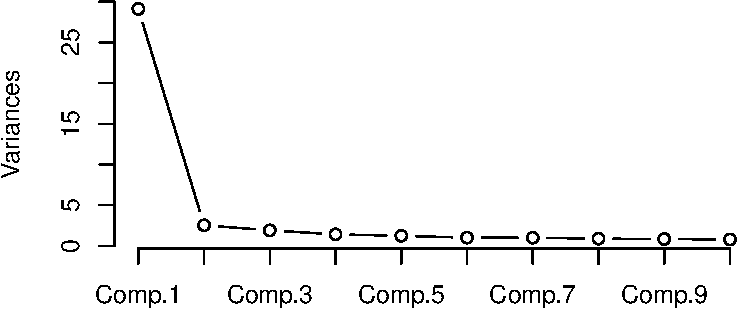
\includegraphics{./results_files/figure-pdf/fig-pca-1.pdf}

}

\caption{\label{fig-pca}Principal Components}

\end{figure}

\hypertarget{proportion-of-variance}{%
\subsection*{Proportion of Variance}\label{proportion-of-variance}}
\addcontentsline{toc}{subsection}{Proportion of Variance}

Second, we estimated a unidimensional Rasch model on dichotomized
responses to the 59 SHAS items and saved the residuals of the person
parameters. We calculated the variance in the observed item responses
and the variance of the residuals. Reckase (1979) suggests that the
unidimensionality assumption is safely met if the Rasch model explains
20\% of the variance in the data. In this case, the proportion of
variance in the SHAS item data explained by the Rasch model was .23.
Thus, the SHAS data meet this criterion.

\hypertarget{principal-component-analysis-of-residuals-pcar}{%
\subsection*{Principal Component Analysis of Residuals
(PCAR)}\label{principal-component-analysis-of-residuals-pcar}}
\addcontentsline{toc}{subsection}{Principal Component Analysis of
Residuals (PCAR)}

Next, we examined the principal components of the correlations among
residuals of the Rasch analysis. The premise is that once the Rasch
model has been estimated, correlations among the item residuals should
be minimal. Linacre () suggests that contrasts with eigenvalues of 2.0
or below can be considered noise. In Figure~\ref{fig-pcar}, our PCAR
analysis found only one contrast that rose above that 2.0 threshold.

\begin{figure}

{\centering 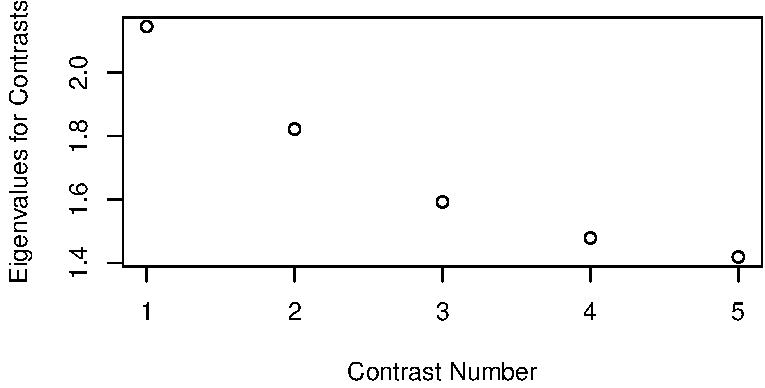
\includegraphics{./results_files/figure-pdf/fig-pcar-1.pdf}

}

\caption{\label{fig-pcar}Contrasts from PCA of Standardized Residual
Correlations}

\end{figure}

\hypertarget{q3}{%
\subsection*{Q3}\label{q3}}
\addcontentsline{toc}{subsection}{Q3}

Finally, we calculated the Q3 statistic {``Effects of Local Item
Dependence on the Fit and Equating Performance of the Three-Parameter
Logistic Model''} (1984) to examine correlations among item residuals,
the premise being that the latent trait should account for so much
common variance in the item responses that any net correlations among
the items should be weak. The Q3 statistic index criteria are that the
raw residual correlation between pairs of items should never exceed 0.10
(Marais \& Andrich, 2008). Of the 1,711 item pairs, the mean correlation
was -0.017 with a standard deviation of 0.035. Thus, most of the
residual correlations among items were very weak. Figure~\ref{fig-q3}
plots the matrix of correlations between item residuals. Each square
depicts a correlation. The squares are shaded in grey with the lightest
shade indicating the weakest correlations. As hoped, the vast majority
of squares are very light, indicating weak correlations among the item
residuals.

\begin{verbatim}

WLE Reliability= 0.918 
Yen's Q3 Statistic based on an estimated theta score 
*** 60 Items | 1770 item pairs
*** Q3 Descriptives
     M     SD    Min    10%    25%    50%    75%    90%    Max 
-0.017  0.036 -0.109 -0.055 -0.040 -0.020 -0.001  0.025  0.321 
\end{verbatim}

\begin{figure}

{\centering 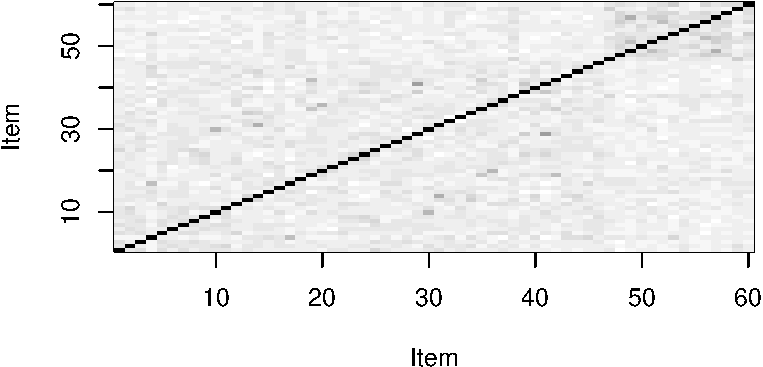
\includegraphics{./results_files/figure-pdf/fig-q3-1.pdf}

}

\caption{\label{fig-q3}Correlation Matrix of Item Residuals}

\end{figure}

\hypertarget{rasch-rating-scale-analysis}{%
\section*{Rasch Rating Scale
Analysis}\label{rasch-rating-scale-analysis}}
\addcontentsline{toc}{section}{Rasch Rating Scale Analysis}

We used the Rasch Rating Scale Model (RSM) (Andrich 1978) to examine the
SHAS item pool. The RSM is a Rasch model (Rasch 1960) that combines (or
``calibrates'') information from items with information from persons to
arrive at a common scale for measuring both an item's and a person's
level of a latent trait, in this case, severity of spiritual abuse. This
scale is expressed in logits (log odds units). Whereas the Rasch model
was designed for use with dichotomous items (0 = incorrect response, 1 =
correct response), the RSM is an extension for use with polytomous items
based on rating scales such as Likert scales of agreement (Embretson and
Reise 2000).

We also use different language from conventional IRT analyses. Because
IRT was developed to measure student achievement, IRT statistics for
both items and persons tend to use language of ``ability'' and
``difficulty.'' For our purpose to measure a psychological trait such as
the experience of spiritual abuse, we chose instead to adopt language of
``severity.'' We used person parameters and scale scores to represent
participants' severity of abuse and to describe item parameters as
severity parameters.

library(tidyverse) library(dplyr) library(tidyr) library(knitr)
library(kableExtra) library(stats4) library(lattice) library(mirt)
library(WrightMap)

The RSM estimates the probability of a person choosing among several
response options (i.e.~Never, Once or twice) given two values: the
severity of abuse represented by the item, and the person's severity of
the latent trait (spiritual abuse). The increase in severity involved in
choosing between two response categories is called a ``step parameter''.
The RSM makes two assumptions of the response categories. One is that
all items use the same rating scale. The other is that the same response
categories distinguish persons equally well for each item. For these
reasons the RSM estimates the same step parameters for all the items.

To convey this information visually, Figure~\ref{fig-RM-plot1} and
Figure~\ref{fig-RM-plot2} are plots of the category response functions
of two items. In both, the horizontal axis is the scale of spiritual
abuse expressed in logits ranging from -2 to +2. The vertical axis is
the probability of selecting a given response (i.e., ``Always'') given
the person's overall severity of spiritual abuse. The blue line is the
probability of selecting Category 1 (``Never'') for persons with less
severe spiritual abuse. Persons with less severe spiritual abuse are
most likely to select ``Never'' while those with more severe abuse are
most likely to select ``Always.'' Between these two extremes are persons
with more moderate or average spiritual abuse. These persons are more
likely to Categories 3 or 4, ``Sometimes'' or ``Often'', respectively.
Both plots show curves that display identical step parameters.

\begin{verbatim}
Iteration in WLE/MLE estimation  1   | Maximal change  2.7551 
Iteration in WLE/MLE estimation  2   | Maximal change  0.8593 
Iteration in WLE/MLE estimation  3   | Maximal change  0.4864 
Iteration in WLE/MLE estimation  4   | Maximal change  0.1926 
Iteration in WLE/MLE estimation  5   | Maximal change  0.028 
Iteration in WLE/MLE estimation  6   | Maximal change  0.0012 
Iteration in WLE/MLE estimation  7   | Maximal change  0 
----
 WLE Reliability= 0.963 
\end{verbatim}

\begin{figure}

{\centering 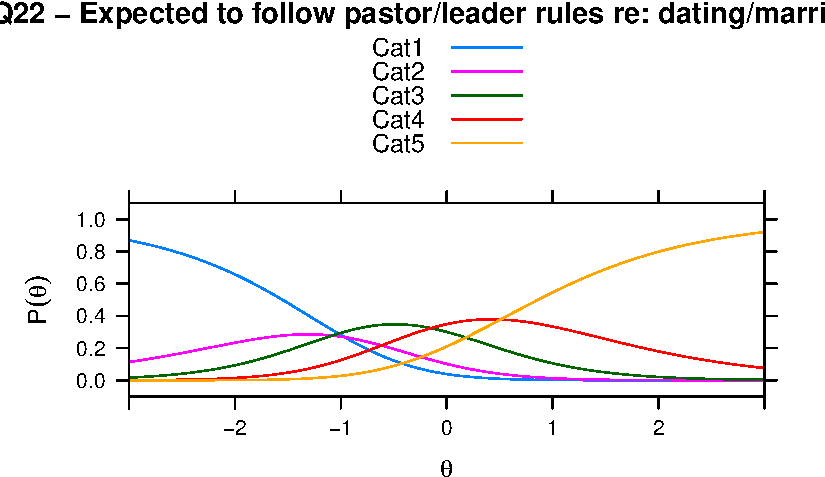
\includegraphics{./results_files/figure-pdf/fig-RM-plot1-1.pdf}

}

\caption{\label{fig-RM-plot1}Category Response Plots}

\end{figure}

\begin{verbatim}
Iteration in WLE/MLE estimation  1   | Maximal change  2.7551 
Iteration in WLE/MLE estimation  2   | Maximal change  0.8593 
Iteration in WLE/MLE estimation  3   | Maximal change  0.4864 
Iteration in WLE/MLE estimation  4   | Maximal change  0.1926 
Iteration in WLE/MLE estimation  5   | Maximal change  0.028 
Iteration in WLE/MLE estimation  6   | Maximal change  0.0012 
Iteration in WLE/MLE estimation  7   | Maximal change  0 
----
 WLE Reliability= 0.963 
\end{verbatim}

\begin{figure}

{\centering 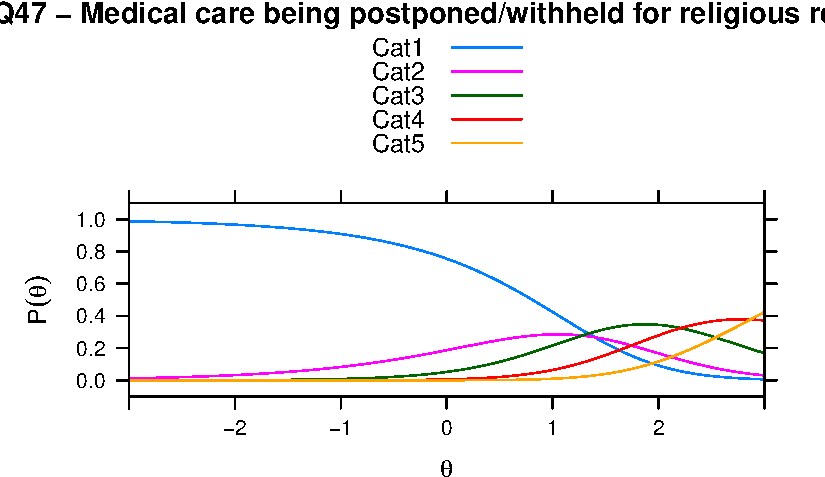
\includegraphics{./results_files/figure-pdf/fig-RM-plot2-1.pdf}

}

\caption{\label{fig-RM-plot2}Category Response Plots}

\end{figure}

These plots point out a step reversal between ``Never'' and ``Once or
twice''. Persons reporting the least severe spiritual abuse were most
likely to report ``Never'' to this prompt of medical care being
postponed or withheld for religious reasons. Persons farther along the
scale who have experienced ``average'' average spiritual abuse should be
more likely to report ``Once or twice'' but were still more likely to
report ``Never''. This finding suggests the ``Never'' and ``Once or
twice'' categories might be collapsed.

\hypertarget{item-severity-parameters-and-fit-statistics}{%
\subsection*{Item Severity Parameters and Fit
Statistics}\label{item-severity-parameters-and-fit-statistics}}
\addcontentsline{toc}{subsection}{Item Severity Parameters and Fit
Statistics}

Table~\ref{tbl-RSM-item-tbl} reports item parameters and fit statistics
for the SHAS items. The first column, xsi, reports the severity
parameter of the item, and we have sorted the items by this value from
least to most severe to facilitate comparison between items.
Table~\ref{tbl-RSM-item-tbl} also reports fit statistics for the items.
These statistics reflect how closely the observed patterns of item
responses fit the patterns of item responses predicted by the RSM. These
fit statistics are chi-square statistics which examine the cumulative
difference the observed pattern of item responses and the pattern of
item responses that the model would expect.

Two fit statistics commonly used in IRT models are the infit mean square
and the outfit mean square (Bond and Fox 2015). The infit statistic
places greater emphasis on unexpected responses that are close to the
persons and item location. The outfit is sensitive to unexpected
responses that are far from the location. The expected value of infit or
outfit for each item is 1.0, with a range of acceptable values ranging
from 0.5 to 1.5. Values outside these boundaries indicate a lack of fit
between items and the model. All but one of the 60 items had infit and
outfit statistics within the acceptable range.

\hypertarget{tbl-RSM-item-tbl}{}
\begin{longtable}[t]{>{\raggedright\arraybackslash}
\caption{\label{tbl-RSM-item-tbl}Estimated Item Parameters for the Rating Scale Model and Item Chi-Square
Fit Statistics }\tabularnewline
p{11cm}ccccc}
\toprule
\multicolumn{2}{c}{ } & \multicolumn{2}{c}{Item Parameters} & \multicolumn{2}{c}{Fit Statistics} \\
\cmidrule(l{3pt}r{3pt}){3-4} \cmidrule(l{3pt}r{3pt}){5-6}
  & subscale & xsi & se.xsi & Outfit & Infit\\
\midrule
\endfirsthead
\multicolumn{6}{@{}l}{\textit{(continued)}}\\
\toprule
  & subscale & xsi & se.xsi & Outfit & Infit\\
\midrule
\endhead

\endfoot
\bottomrule
\endlastfoot
*EQ22 - Expected to follow pastor/leader rules re: dating/marriage/sex & controlling leadership & -0.42 & 0.02 & 1.20 & 1.25\\
EQ66 - Others treated as less than due to their sexual orientation &  & -0.35 & 0.02 & 1.10 & 1.05\\
EQ25 - Feeling unable to raise questions and issues &  & -0.26 & 0.02 & 0.77 & 0.76\\
EQ35 - Taught to distrust my emotions &  & -0.19 & 0.02 & 1.06 & 0.97\\
*IQ77 - Anger upon reflecting on negative religious experiences & internal distress & -0.13 & 0.02 & 0.71 & 0.68\\
\addlinespace
EQ39 - Made to feel shame over natural sexual desires (not actions) &  & -0.12 & 0.02 & 1.12 & 1.12\\
*IQ80 - Feeling isolated & internal distress & -0.11 & 0.02 & 0.94 & 0.87\\
*IQ69 - Lack of spiritual direction/purpose & internal distress & -0.05 & 0.02 & 1.34 & 1.12\\
*IQ71 - Avoiding religious activities/settings to reduce distressing feelings & internal distress & -0.04 & 0.02 & 0.92 & 0.92\\
EQ38 - Unrealistic demands placed on my moral/religious behavior &  & 0.00 & 0.02 & 0.75 & 0.78\\
\addlinespace
EQ37 - Made to feel less spiritually mature than pastor/leadership &  & 0.01 & 0.02 & 0.91 & 0.90\\
EQ54 - Being explicitly taught to distrust my intuitions &  & 0.03 & 0.02 & 0.95 & 0.93\\
IQ76 - Feeling I wasted years of my life in a church/set of beliefs &  & 0.15 & 0.02 & 1.06 & 1.09\\
EQ32 - Feeling unable to express unhappiness &  & 0.17 & 0.02 & 0.91 & 0.89\\
EQ61 - Developmentally-inappropriate/anxious end times descriptions taught to young children &  & 0.18 & 0.02 & 1.11 & 1.14\\
\addlinespace
EQ36 - Mental/physical problems interpreted as spiritual/moral weakness &  & 0.18 & 0.02 & 0.83 & 0.82\\
*IQ74 - Sadness over the loss of my faith/religious community & internal distress & 0.19 & 0.02 & 1.33 & 1.18\\
*EQ45 - Developmentally-inappropriate/anxious Hell/Satan/demons taught to young children & spiritual violence & 0.20 & 0.02 & 1.08 & 1.10\\
*IQ78 - A lack of self-worth & internal distress & 0.20 & 0.02 & 1.09 & 1.02\\
EQ18 - Church/pastor discourage critical thinking &  & 0.22 & 0.02 & 0.82 & 0.84\\
\addlinespace
EQ56 - Being made to feel I was crazy/weird for doubts/questions &  & 0.24 & 0.02 & 0.67 & 0.71\\
EQ44 - Love/acceptance offered only for high spiritual/moral performance &  & 0.36 & 0.02 & 0.77 & 0.76\\
EQ42 - Seeing others shamed/shunned by pastor/leader/group &  & 0.38 & 0.02 & 0.75 & 0.73\\
*EQ7 - Pastor speaking on God's behalf & controlling leadership & 0.45 & 0.02 & 1.38 & 1.26\\
*EQ58 - Terror/horror used to motivate religious decisions & spiritual violence & 0.45 & 0.02 & 0.91 & 0.94\\
\addlinespace
EQ11 - Disagree w/pastor portrayed as evil &  & 0.47 & 0.02 & 0.83 & 0.85\\
*IQ73 - Self-hatred or self-loathing & internal distress & 0.51 & 0.02 & 1.18 & 1.16\\
EQ29 - Feeling special when in pastor’s good graces; otherwise ignored &  & 0.52 & 0.02 & 1.11 & 1.08\\
*EQ34 - Scripture used to justify physical punishment/severe discipline & spiritual violence & 0.53 & 0.02 & 1.21 & 1.18\\
*IQ79 - Distrust of God & harmful God-image & 0.62 & 0.02 & 1.34 & 1.20\\
\addlinespace
EQ53 - Scripture used to justify abusive parent-child behavior &  & 0.64 & 0.02 & 0.96 & 1.01\\
*EQ51 - Extreme pressure to be pastor/missionary/spiritual leader & controlling leadership & 0.67 & 0.02 & 1.40 & 1.38\\
*EQ19 - Behavior excessively monitored by pastor/group & controlling leadership & 0.69 & 0.02 & 0.86 & 0.93\\
EQ63 - Shamed by pastor/group for raising questions or concerns &  & 0.72 & 0.02 & 0.75 & 0.78\\
EQ40 - Threatening Divine punishment to keep group members in line &  & 0.74 & 0.02 & 0.93 & 1.02\\
\addlinespace
*EQ28 - Leadershi/group protecting abusive individuals & maintain system & 0.76 & 0.02 & 0.93 & 0.91\\
EQ64 - Witnessing women pressured to stay in unfaithful/abusive marriages &  & 0.77 & 0.02 & 1.00 & 1.00\\
EQ50 - Treated as less than because of my gender & gender discrimination & 0.79 & 0.02 & 1.96 & 1.93\\
*IQ82 - Having trouble navigating life outside my church/community & internal distress & 0.80 & 0.02 & 1.17 & 1.15\\
EQ21 - Taught I would risk Hell if left my church/group &  & 0.83 & 0.02 & 1.30 & 1.39\\
\addlinespace
EQ59 - Pastor/group blame victim for their abuse &  & 0.87 & 0.02 & 0.76 & 0.81\\
*EQ62 - Scripture used to justify physical violence & spiritual violence & 0.88 & 0.02 & 1.08 & 1.11\\
EQ20 - Members pressured to give money despite financial hardship &  & 0.88 & 0.02 & 1.14 & 1.27\\
EQ57 - Developing mental/physical ailments from conforming to group/leader’s expectation &  & 0.89 & 0.02 & 0.94 & 1.08\\
*EQ16 - Church/community abandoning me in difficult time & maintain system & 0.92 & 0.02 & 1.03 & 1.06\\
\addlinespace
EQ49 - Leadership/group protecting and elevating abusive individuals &  & 0.92 & 0.02 & 0.89 & 0.93\\
*IQ70 - Feeling betrayed by God & harmful God-image & 0.95 & 0.02 & 1.37 & 1.27\\
*EQ52 - Blamed for harm I suffered rather than blaming who harmed me & maintain system & 0.98 & 0.02 & 0.80 & 0.89\\
IQ68 - Anxiety attacks triggered by religious stimuli &  & 1.03 & 0.02 & 0.97 & 1.06\\
EQ30 - Deterred from seeking mental health treatment/counseling/medication &  & 1.03 & 0.02 & 0.96 & 1.03\\
\addlinespace
EQ43 - Shamed by pastor/group for poor spiritual/moral performance &  & 1.03 & 0.02 & 0.81 & 0.84\\
*EQ31 - Shunned/ignored by pastor/church/group & maintain system & 1.04 & 0.02 & 1.14 & 1.09\\
EQ23 - Prayer replacing needed medical interventions &  & 1.19 & 0.02 & 1.10 & 1.09\\
*EQ24 - Expected to consult pastor/leader before making non-religious decisions & controlling leadership & 1.24 & 0.02 & 1.02 & 1.08\\
*EQ26 - Pressured to forgive abuser while abuse was ongoing & maintain system & 1.26 & 0.02 & 1.37 & 1.30\\
\addlinespace
EQ10 - Asked to give up personal goals by pastor &  & 1.32 & 0.02 & 1.11 & 1.19\\
EQ65 - Cut off/shunned by more religious family members &  & 1.33 & 0.02 & 1.26 & 1.25\\
IQ81 - Nightmares about my negative religious experiences &  & 1.42 & 0.02 & 0.90 & 0.97\\
*IQ72 - Feeling as if God harmed me directly & harmful God-image & 1.64 & 0.02 & 1.14 & 1.22\\
EQ47 - Medical care being postponed/withheld for religious reasons &  & 1.94 & 0.03 & 1.10 & 1.16\\*
\end{longtable}

\begin{figure}

{\centering 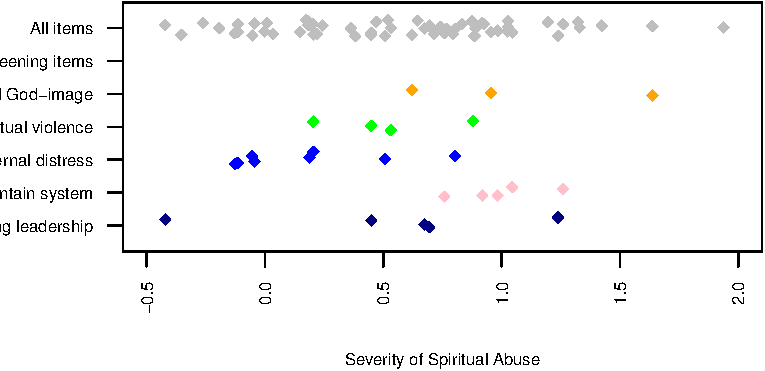
\includegraphics{./results_files/figure-pdf/fig-RSM-item-histogram-1.pdf}

}

\caption{\label{fig-RSM-item-histogram}Distribution of Item Severity
Parameters}

\end{figure}

\hypertarget{reliability}{%
\subsection*{Reliability}\label{reliability}}
\addcontentsline{toc}{subsection}{Reliability}

The RSM expresses internal consistency reliability as Rasch person
separation. Based on Table X, the SHAS has a high Rasch person
separation reliability value of .963, indicating that the estimated RSM
scale discriminated well between persons with varying severity of
spiritual abuse.

The SHAS also has a high Rasch item separation reliability with Rel =
.XX, χ2 (XX) = XXXX.X, p \textless{} .XX, implying that the items have a
good spread in terms of item ordering and hierarchy.

\hypertarget{item-person-map}{%
\subsection*{Item-Person Map}\label{item-person-map}}
\addcontentsline{toc}{subsection}{Item-Person Map}

Figure~\ref{fig-RSM-WrightMap} displays an item-person map (also called
a ``Wright map'') that shows the item severities of the SHAS items and
the person severities for each person who completed the survey. All
these severities are estimated in logits (log odds units) as the unit of
measures. This means the higher the logit value for an item is, the less
likely it was for a person to endorse that particular item. On the other
hand, higher logit values for each person indicate more severe spiritual
abuse. On the variable map, the mean item severity is constrained to be
0.00 with person severities being relative to that mean item severity
While column 1 shows the latent continuum in terms of logit values as
the unit of measurement underlying the SHAS, columns 2 and 3 represent
the severities of the people and the items.

Figure~\ref{fig-RSM-WrightMap} shows good overlap between the person
trait and item severity as evidenced by the match between the mean of
the person severity (M = − 0.58) and the mean of the item severity (M =
0.00). This suggests that the majority of the items were appropriate for
the sample. While person severity measures range from X.XX logits to −
X.XX logits (M = − 0.XX, SD = 0.XX, N = XXXX), the item severities range
from X.XX logits to − X.XX logits (M = X.XX, SD = 0.XX, N = XXXX). The
item representing the most severe spiritual abuse for participants is
Item X, ``I feel \ldots{} XXX'' with the severity at X.XX logits (also
reported in Appendix Table 2). By contrast the item representing the
least severe spiritual abuse is item XX, ``I would \ldots{}'', with −
1.08 logits.

\begin{figure}

{\centering 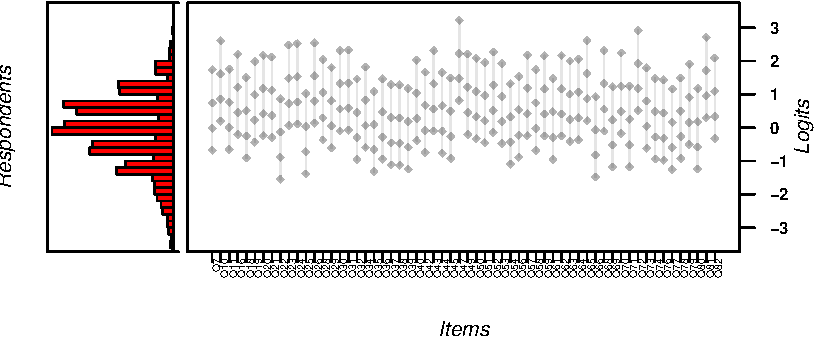
\includegraphics{./results_files/figure-pdf/fig-RSM-WrightMap-1.pdf}

}

\caption{\label{fig-RSM-WrightMap}Item-Person Map}

\end{figure}

\hypertarget{model-data-fit}{%
\subsection*{Model-Data Fit}\label{model-data-fit}}
\addcontentsline{toc}{subsection}{Model-Data Fit}

To assess the overall fit of the RSM to the SHAS item response data, we
use two statistics. The first is the Root Mean Square Error of
Approximation (RMSEA). The suggested cutoff for RMSEA is .06. The second
is the CFI. The suggested cutoff for the CFI is .95. These fit
statistics are presented in \textbf{?@tbl-RSM-model-fit}.

\begin{table}

\caption{\textbf{?(caption)}}\begin{minipage}[t]{\linewidth}

{\centering 

\begin{verbatim}
'log Lik.' -225573.6 (df=64)
\end{verbatim}

}

\end{minipage}%

\end{table}

The obtained RMSEA value of .09 (95\% CI{[}.092, .093{]}) exceeds the
cutoff of .06. The CFI of .953 meets the recommended .95 threshold.
Together these statistics evidence that the RSM fits the SHAS items.

\hypertarget{dif-analysis}{%
\section*{DIF Analysis}\label{dif-analysis}}
\addcontentsline{toc}{section}{DIF Analysis}

Differential item functioning (DIF) examines how an item functions
differently for people of equal standing on the trait. In this case, we
conducted DIF analysis of the SHAS items to examine item bias by gender,
and age, and race. {[}We applied logistic ordinal regression with IRT
scoring. {[}We used the Chi-squared likelihood-ratio statistic as the
initial DIF detection criteria (alpha \textless{} 0.01) and a cut-off of
McFadden pseudo R2Δ ≥ 0.02 in model comparisons to determine substantial
DIF, a reasonable threshold used in the development of self-reported
health outcomes.{]}

\begin{verbatim}

Iteration: 1, Log-Lik: -213318.816, Max-Change: 1.97479
Iteration: 2, Log-Lik: -207326.915, Max-Change: 0.78632
Iteration: 3, Log-Lik: -206827.051, Max-Change: 0.14588
Iteration: 4, Log-Lik: -206716.928, Max-Change: 0.20478
Iteration: 5, Log-Lik: -206638.290, Max-Change: 0.18581
Iteration: 6, Log-Lik: -206576.440, Max-Change: 0.20030
Iteration: 7, Log-Lik: -206520.234, Max-Change: 0.20248
Iteration: 8, Log-Lik: -206473.738, Max-Change: 0.19881
Iteration: 9, Log-Lik: -206431.582, Max-Change: 0.19055
Iteration: 10, Log-Lik: -206395.065, Max-Change: 0.18567
Iteration: 11, Log-Lik: -206364.147, Max-Change: 0.36756
Iteration: 12, Log-Lik: -206295.370, Max-Change: 0.22522
Iteration: 13, Log-Lik: -206270.523, Max-Change: 0.15986
Iteration: 14, Log-Lik: -206247.418, Max-Change: 0.20072
Iteration: 15, Log-Lik: -206228.098, Max-Change: 0.18190
Iteration: 16, Log-Lik: -206210.358, Max-Change: 0.15196
Iteration: 17, Log-Lik: -206193.523, Max-Change: 0.13424
Iteration: 18, Log-Lik: -206178.731, Max-Change: 0.11090
Iteration: 19, Log-Lik: -206164.318, Max-Change: 0.12232
Iteration: 20, Log-Lik: -206151.746, Max-Change: 0.10973
Iteration: 21, Log-Lik: -206139.934, Max-Change: 0.10888
Iteration: 22, Log-Lik: -206129.186, Max-Change: 0.09991
Iteration: 23, Log-Lik: -206119.191, Max-Change: 0.09902
Iteration: 24, Log-Lik: -206110.082, Max-Change: 0.09119
Iteration: 25, Log-Lik: -206101.578, Max-Change: 0.09067
Iteration: 26, Log-Lik: -206093.823, Max-Change: 0.08374
Iteration: 27, Log-Lik: -206086.563, Max-Change: 0.08330
Iteration: 28, Log-Lik: -206079.933, Max-Change: 0.07733
Iteration: 29, Log-Lik: -206073.715, Max-Change: 0.07723
Iteration: 30, Log-Lik: -206068.031, Max-Change: 0.07247
Iteration: 31, Log-Lik: -206062.692, Max-Change: 0.07296
Iteration: 32, Log-Lik: -206057.810, Max-Change: 0.06925
Iteration: 33, Log-Lik: -206053.219, Max-Change: 0.07012
Iteration: 34, Log-Lik: -206050.472, Max-Change: 0.03063
Iteration: 35, Log-Lik: -206045.892, Max-Change: 0.02322
Iteration: 36, Log-Lik: -206041.820, Max-Change: 0.01988
Iteration: 37, Log-Lik: -206032.733, Max-Change: 0.02755
Iteration: 38, Log-Lik: -206027.119, Max-Change: 0.03479
Iteration: 39, Log-Lik: -206022.114, Max-Change: 0.03620
Iteration: 40, Log-Lik: -206019.922, Max-Change: 0.03688
Iteration: 41, Log-Lik: -206015.800, Max-Change: 0.02438
Iteration: 42, Log-Lik: -206013.984, Max-Change: 0.01205
Iteration: 43, Log-Lik: -206010.997, Max-Change: 0.01116
Iteration: 44, Log-Lik: -206008.752, Max-Change: 0.01087
Iteration: 45, Log-Lik: -206006.704, Max-Change: 0.00975
Iteration: 46, Log-Lik: -205997.586, Max-Change: 0.01197
Iteration: 47, Log-Lik: -205996.528, Max-Change: 0.00841
Iteration: 48, Log-Lik: -205995.470, Max-Change: 0.00622
Iteration: 49, Log-Lik: -205994.488, Max-Change: 0.00584
Iteration: 50, Log-Lik: -205993.804, Max-Change: 0.00559
Iteration: 51, Log-Lik: -205993.195, Max-Change: 0.00558
Iteration: 52, Log-Lik: -205989.948, Max-Change: 0.00611
Iteration: 53, Log-Lik: -205989.587, Max-Change: 0.00410
Iteration: 54, Log-Lik: -205989.252, Max-Change: 0.00433
Iteration: 55, Log-Lik: -205987.937, Max-Change: 0.00314
Iteration: 56, Log-Lik: -205987.736, Max-Change: 0.00311
Iteration: 57, Log-Lik: -205987.542, Max-Change: 0.00323
Iteration: 58, Log-Lik: -205986.823, Max-Change: 0.00841
Iteration: 59, Log-Lik: -205986.770, Max-Change: 0.00530
Iteration: 60, Log-Lik: -205986.573, Max-Change: 0.00196
Iteration: 61, Log-Lik: -205986.451, Max-Change: 0.00250
Iteration: 62, Log-Lik: -205986.338, Max-Change: 0.00188
Iteration: 63, Log-Lik: -205986.253, Max-Change: 0.00217
Iteration: 64, Log-Lik: -205986.073, Max-Change: 0.00173
Iteration: 65, Log-Lik: -205985.983, Max-Change: 0.00159
Iteration: 66, Log-Lik: -205985.906, Max-Change: 0.00166
Iteration: 67, Log-Lik: -205985.526, Max-Change: 0.00522
Iteration: 68, Log-Lik: -205985.435, Max-Change: 0.00134
Iteration: 69, Log-Lik: -205985.382, Max-Change: 0.00120
Iteration: 70, Log-Lik: -205985.311, Max-Change: 0.00137
Iteration: 71, Log-Lik: -205985.265, Max-Change: 0.00154
Iteration: 72, Log-Lik: -205985.226, Max-Change: 0.00215
Iteration: 73, Log-Lik: -205985.162, Max-Change: 0.00133
Iteration: 74, Log-Lik: -205985.118, Max-Change: 0.00137
Iteration: 75, Log-Lik: -205985.092, Max-Change: 0.00136
Iteration: 76, Log-Lik: -205985.047, Max-Change: 0.00339
Iteration: 77, Log-Lik: -205985.022, Max-Change: 0.00324
Iteration: 78, Log-Lik: -205985.000, Max-Change: 0.00406
Iteration: 79, Log-Lik: -205984.981, Max-Change: 0.00164
Iteration: 80, Log-Lik: -205984.940, Max-Change: 0.00059
Iteration: 81, Log-Lik: -205984.922, Max-Change: 0.00198
Iteration: 82, Log-Lik: -205984.923, Max-Change: 0.00262
Iteration: 83, Log-Lik: -205984.880, Max-Change: 0.00055
Iteration: 84, Log-Lik: -205984.864, Max-Change: 0.00156
Iteration: 85, Log-Lik: -205984.864, Max-Change: 0.00279
Iteration: 86, Log-Lik: -205984.826, Max-Change: 0.00077
Iteration: 87, Log-Lik: -205984.811, Max-Change: 0.00109
Iteration: 88, Log-Lik: -205984.753, Max-Change: 0.00208
Iteration: 89, Log-Lik: -205984.721, Max-Change: 0.00070
Iteration: 90, Log-Lik: -205984.704, Max-Change: 0.00160
Iteration: 91, Log-Lik: -205984.700, Max-Change: 0.00128
Iteration: 92, Log-Lik: -205984.675, Max-Change: 0.00079
Iteration: 93, Log-Lik: -205984.660, Max-Change: 0.00064
Iteration: 94, Log-Lik: -205984.647, Max-Change: 0.00036
Iteration: 95, Log-Lik: -205984.645, Max-Change: 0.00045
Iteration: 96, Log-Lik: -205984.636, Max-Change: 0.00043
Iteration: 97, Log-Lik: -205984.635, Max-Change: 0.00167
Iteration: 98, Log-Lik: -205984.633, Max-Change: 0.00097
Iteration: 99, Log-Lik: -205984.615, Max-Change: 0.00047
Iteration: 100, Log-Lik: -205984.615, Max-Change: 0.00039
Iteration: 101, Log-Lik: -205984.613, Max-Change: 0.00041
Iteration: 102, Log-Lik: -205984.604, Max-Change: 0.00121
Iteration: 103, Log-Lik: -205984.602, Max-Change: 0.00173
Iteration: 104, Log-Lik: -205984.582, Max-Change: 0.00108
Iteration: 105, Log-Lik: -205984.570, Max-Change: 0.00094
Iteration: 106, Log-Lik: -205984.530, Max-Change: 0.00216
Iteration: 107, Log-Lik: -205984.509, Max-Change: 0.00200
Iteration: 108, Log-Lik: -205984.507, Max-Change: 0.00207
Iteration: 109, Log-Lik: -205984.499, Max-Change: 0.00061
Iteration: 110, Log-Lik: -205984.497, Max-Change: 0.00082
Iteration: 111, Log-Lik: -205984.489, Max-Change: 0.00035
Iteration: 112, Log-Lik: -205984.489, Max-Change: 0.00027
Iteration: 113, Log-Lik: -205984.488, Max-Change: 0.00039
Iteration: 114, Log-Lik: -205984.481, Max-Change: 0.00039
Iteration: 115, Log-Lik: -205984.481, Max-Change: 0.00030
Iteration: 116, Log-Lik: -205984.480, Max-Change: 0.00047
Iteration: 117, Log-Lik: -205984.474, Max-Change: 0.00040
Iteration: 118, Log-Lik: -205984.474, Max-Change: 0.00029
Iteration: 119, Log-Lik: -205984.472, Max-Change: 0.00033
Iteration: 120, Log-Lik: -205984.466, Max-Change: 0.00029
Iteration: 121, Log-Lik: -205984.466, Max-Change: 0.00113
Iteration: 122, Log-Lik: -205984.464, Max-Change: 0.00072
Iteration: 123, Log-Lik: -205984.453, Max-Change: 0.00025
Iteration: 124, Log-Lik: -205984.452, Max-Change: 0.00110
Iteration: 125, Log-Lik: -205984.451, Max-Change: 0.00087
Iteration: 126, Log-Lik: -205984.439, Max-Change: 0.00035
Iteration: 127, Log-Lik: -205984.439, Max-Change: 0.00031
Iteration: 128, Log-Lik: -205984.438, Max-Change: 0.00044
Iteration: 129, Log-Lik: -205984.432, Max-Change: 0.00037
Iteration: 130, Log-Lik: -205984.432, Max-Change: 0.00027
Iteration: 131, Log-Lik: -205984.431, Max-Change: 0.00032
Iteration: 132, Log-Lik: -205984.426, Max-Change: 0.00027
Iteration: 133, Log-Lik: -205984.426, Max-Change: 0.00107
Iteration: 134, Log-Lik: -205984.423, Max-Change: 0.00089
Iteration: 135, Log-Lik: -205984.421, Max-Change: 0.00067
Iteration: 136, Log-Lik: -205984.418, Max-Change: 0.00048
Iteration: 137, Log-Lik: -205984.416, Max-Change: 0.00040
Iteration: 138, Log-Lik: -205984.413, Max-Change: 0.00028
Iteration: 139, Log-Lik: -205984.412, Max-Change: 0.00093
Iteration: 140, Log-Lik: -205984.410, Max-Change: 0.00093
Iteration: 141, Log-Lik: -205984.408, Max-Change: 0.00057
Iteration: 142, Log-Lik: -205984.405, Max-Change: 0.00049
Iteration: 143, Log-Lik: -205984.403, Max-Change: 0.00034
Iteration: 144, Log-Lik: -205984.400, Max-Change: 0.00029
Iteration: 145, Log-Lik: -205984.400, Max-Change: 0.00101
Iteration: 146, Log-Lik: -205984.398, Max-Change: 0.00084
Iteration: 147, Log-Lik: -205984.395, Max-Change: 0.00063
Iteration: 148, Log-Lik: -205984.392, Max-Change: 0.00046
Iteration: 149, Log-Lik: -205984.391, Max-Change: 0.00038
Iteration: 150, Log-Lik: -205984.388, Max-Change: 0.00026
Iteration: 151, Log-Lik: -205984.388, Max-Change: 0.00088
Iteration: 152, Log-Lik: -205984.386, Max-Change: 0.00088
Iteration: 153, Log-Lik: -205984.383, Max-Change: 0.00054
Iteration: 154, Log-Lik: -205984.381, Max-Change: 0.00047
Iteration: 155, Log-Lik: -205984.379, Max-Change: 0.00032
Iteration: 156, Log-Lik: -205984.376, Max-Change: 0.00028
Iteration: 157, Log-Lik: -205984.376, Max-Change: 0.00096
Iteration: 158, Log-Lik: -205984.374, Max-Change: 0.00080
Iteration: 159, Log-Lik: -205984.372, Max-Change: 0.00060
Iteration: 160, Log-Lik: -205984.369, Max-Change: 0.00044
Iteration: 161, Log-Lik: -205984.368, Max-Change: 0.00036
Iteration: 162, Log-Lik: -205984.365, Max-Change: 0.00025
Iteration: 163, Log-Lik: -205984.365, Max-Change: 0.00084
Iteration: 164, Log-Lik: -205984.363, Max-Change: 0.00084
Iteration: 165, Log-Lik: -205984.361, Max-Change: 0.00051
Iteration: 166, Log-Lik: -205984.359, Max-Change: 0.00045
Iteration: 167, Log-Lik: -205984.358, Max-Change: 0.00031
Iteration: 168, Log-Lik: -205984.355, Max-Change: 0.00027
Iteration: 169, Log-Lik: -205984.354, Max-Change: 0.00092
Iteration: 170, Log-Lik: -205984.353, Max-Change: 0.00077
Iteration: 171, Log-Lik: -205984.351, Max-Change: 0.00058
Iteration: 172, Log-Lik: -205984.348, Max-Change: 0.00042
Iteration: 173, Log-Lik: -205984.347, Max-Change: 0.00035
Iteration: 174, Log-Lik: -205984.344, Max-Change: 0.00024
Iteration: 175, Log-Lik: -205984.344, Max-Change: 0.00081
Iteration: 176, Log-Lik: -205984.343, Max-Change: 0.00081
Iteration: 177, Log-Lik: -205984.340, Max-Change: 0.00049
Iteration: 178, Log-Lik: -205984.338, Max-Change: 0.00043
Iteration: 179, Log-Lik: -205984.337, Max-Change: 0.00029
Iteration: 180, Log-Lik: -205984.334, Max-Change: 0.00026
Iteration: 181, Log-Lik: -205984.334, Max-Change: 0.00088
Iteration: 182, Log-Lik: -205984.333, Max-Change: 0.00074
Iteration: 183, Log-Lik: -205984.331, Max-Change: 0.00056
Iteration: 184, Log-Lik: -205984.329, Max-Change: 0.00040
Iteration: 185, Log-Lik: -205984.328, Max-Change: 0.00034
Iteration: 186, Log-Lik: -205984.325, Max-Change: 0.00023
Iteration: 187, Log-Lik: -205984.325, Max-Change: 0.00078
Iteration: 188, Log-Lik: -205984.323, Max-Change: 0.00078
Iteration: 189, Log-Lik: -205984.321, Max-Change: 0.00047
Iteration: 190, Log-Lik: -205984.319, Max-Change: 0.00041
Iteration: 191, Log-Lik: -205984.318, Max-Change: 0.00028
Iteration: 192, Log-Lik: -205984.316, Max-Change: 0.00025
Iteration: 193, Log-Lik: -205984.316, Max-Change: 0.00085
Iteration: 194, Log-Lik: -205984.314, Max-Change: 0.00071
Iteration: 195, Log-Lik: -205984.312, Max-Change: 0.00054
Iteration: 196, Log-Lik: -205984.310, Max-Change: 0.00039
Iteration: 197, Log-Lik: -205984.309, Max-Change: 0.00032
Iteration: 198, Log-Lik: -205984.307, Max-Change: 0.00022
Iteration: 199, Log-Lik: -205984.307, Max-Change: 0.00075
Iteration: 200, Log-Lik: -205984.305, Max-Change: 0.00075
Iteration: 201, Log-Lik: -205984.304, Max-Change: 0.00046
Iteration: 202, Log-Lik: -205984.302, Max-Change: 0.00040
Iteration: 203, Log-Lik: -205984.301, Max-Change: 0.00027
Iteration: 204, Log-Lik: -205984.298, Max-Change: 0.00024
Iteration: 205, Log-Lik: -205984.298, Max-Change: 0.00082
Iteration: 206, Log-Lik: -205984.297, Max-Change: 0.00069
Iteration: 207, Log-Lik: -205984.295, Max-Change: 0.00052
Iteration: 208, Log-Lik: -205984.293, Max-Change: 0.00037
Iteration: 209, Log-Lik: -205984.292, Max-Change: 0.00031
Iteration: 210, Log-Lik: -205984.290, Max-Change: 0.00022
Iteration: 211, Log-Lik: -205984.290, Max-Change: 0.00072
Iteration: 212, Log-Lik: -205984.289, Max-Change: 0.00072
Iteration: 213, Log-Lik: -205984.287, Max-Change: 0.00044
Iteration: 214, Log-Lik: -205984.285, Max-Change: 0.00039
Iteration: 215, Log-Lik: -205984.284, Max-Change: 0.00026
Iteration: 216, Log-Lik: -205984.282, Max-Change: 0.00023
Iteration: 217, Log-Lik: -205984.282, Max-Change: 0.00079
Iteration: 218, Log-Lik: -205984.281, Max-Change: 0.00066
Iteration: 219, Log-Lik: -205984.279, Max-Change: 0.00050
Iteration: 220, Log-Lik: -205984.277, Max-Change: 0.00036
Iteration: 221, Log-Lik: -205984.277, Max-Change: 0.00030
Iteration: 222, Log-Lik: -205984.275, Max-Change: 0.00021
Iteration: 223, Log-Lik: -205984.274, Max-Change: 0.00070
Iteration: 224, Log-Lik: -205984.273, Max-Change: 0.00070
Iteration: 225, Log-Lik: -205984.272, Max-Change: 0.00043
Iteration: 226, Log-Lik: -205984.270, Max-Change: 0.00037
Iteration: 227, Log-Lik: -205984.269, Max-Change: 0.00026
Iteration: 228, Log-Lik: -205984.267, Max-Change: 0.00022
Iteration: 229, Log-Lik: -205984.267, Max-Change: 0.00077
Iteration: 230, Log-Lik: -205984.266, Max-Change: 0.00064
Iteration: 231, Log-Lik: -205984.264, Max-Change: 0.00048
Iteration: 232, Log-Lik: -205984.263, Max-Change: 0.00035
Iteration: 233, Log-Lik: -205984.262, Max-Change: 0.00029
Iteration: 234, Log-Lik: -205984.260, Max-Change: 0.00020
Iteration: 235, Log-Lik: -205984.260, Max-Change: 0.00067
Iteration: 236, Log-Lik: -205984.259, Max-Change: 0.00067
Iteration: 237, Log-Lik: -205984.257, Max-Change: 0.00041
Iteration: 238, Log-Lik: -205984.256, Max-Change: 0.00036
Iteration: 239, Log-Lik: -205984.255, Max-Change: 0.00025
Iteration: 240, Log-Lik: -205984.253, Max-Change: 0.00021
Iteration: 241, Log-Lik: -205984.253, Max-Change: 0.00074
Iteration: 242, Log-Lik: -205984.252, Max-Change: 0.00062
Iteration: 243, Log-Lik: -205984.250, Max-Change: 0.00047
Iteration: 244, Log-Lik: -205984.249, Max-Change: 0.00034
Iteration: 245, Log-Lik: -205984.248, Max-Change: 0.00028
Iteration: 246, Log-Lik: -205984.246, Max-Change: 0.00019
Iteration: 247, Log-Lik: -205984.246, Max-Change: 0.00065
Iteration: 248, Log-Lik: -205984.245, Max-Change: 0.00065
Iteration: 249, Log-Lik: -205984.244, Max-Change: 0.00040
Iteration: 250, Log-Lik: -205984.242, Max-Change: 0.00035
Iteration: 251, Log-Lik: -205984.242, Max-Change: 0.00024
Iteration: 252, Log-Lik: -205984.240, Max-Change: 0.00021
Iteration: 253, Log-Lik: -205984.240, Max-Change: 0.00072
Iteration: 254, Log-Lik: -205984.239, Max-Change: 0.00060
Iteration: 255, Log-Lik: -205984.237, Max-Change: 0.00045
Iteration: 256, Log-Lik: -205984.236, Max-Change: 0.00032
Iteration: 257, Log-Lik: -205984.235, Max-Change: 0.00027
Iteration: 258, Log-Lik: -205984.234, Max-Change: 0.00019
Iteration: 259, Log-Lik: -205984.233, Max-Change: 0.00063
Iteration: 260, Log-Lik: -205984.233, Max-Change: 0.00063
Iteration: 261, Log-Lik: -205984.231, Max-Change: 0.00038
Iteration: 262, Log-Lik: -205984.230, Max-Change: 0.00034
Iteration: 263, Log-Lik: -205984.229, Max-Change: 0.00023
Iteration: 264, Log-Lik: -205984.228, Max-Change: 0.00020
Iteration: 265, Log-Lik: -205984.227, Max-Change: 0.00069
Iteration: 266, Log-Lik: -205984.227, Max-Change: 0.00058
Iteration: 267, Log-Lik: -205984.225, Max-Change: 0.00044
Iteration: 268, Log-Lik: -205984.224, Max-Change: 0.00031
Iteration: 269, Log-Lik: -205984.223, Max-Change: 0.00026
Iteration: 270, Log-Lik: -205984.222, Max-Change: 0.00018
Iteration: 271, Log-Lik: -205984.222, Max-Change: 0.00061
Iteration: 272, Log-Lik: -205984.221, Max-Change: 0.00061
Iteration: 273, Log-Lik: -205984.220, Max-Change: 0.00037
Iteration: 274, Log-Lik: -205984.218, Max-Change: 0.00033
Iteration: 275, Log-Lik: -205984.218, Max-Change: 0.00022
Iteration: 276, Log-Lik: -205984.216, Max-Change: 0.00019
Iteration: 277, Log-Lik: -205984.216, Max-Change: 0.00067
Iteration: 278, Log-Lik: -205984.215, Max-Change: 0.00056
Iteration: 279, Log-Lik: -205984.214, Max-Change: 0.00042
Iteration: 280, Log-Lik: -205984.213, Max-Change: 0.00030
Iteration: 281, Log-Lik: -205984.212, Max-Change: 0.00025
Iteration: 282, Log-Lik: -205984.211, Max-Change: 0.00017
Iteration: 283, Log-Lik: -205984.210, Max-Change: 0.00059
Iteration: 284, Log-Lik: -205984.210, Max-Change: 0.00059
Iteration: 285, Log-Lik: -205984.209, Max-Change: 0.00036
Iteration: 286, Log-Lik: -205984.207, Max-Change: 0.00032
Iteration: 287, Log-Lik: -205984.207, Max-Change: 0.00022
Iteration: 288, Log-Lik: -205984.205, Max-Change: 0.00019
Iteration: 289, Log-Lik: -205984.205, Max-Change: 0.00065
Iteration: 290, Log-Lik: -205984.204, Max-Change: 0.00054
Iteration: 291, Log-Lik: -205984.203, Max-Change: 0.00041
Iteration: 292, Log-Lik: -205984.202, Max-Change: 0.00029
Iteration: 293, Log-Lik: -205984.202, Max-Change: 0.00025
Iteration: 294, Log-Lik: -205984.200, Max-Change: 0.00017
Iteration: 295, Log-Lik: -205984.200, Max-Change: 0.00057
Iteration: 296, Log-Lik: -205984.199, Max-Change: 0.00057
Iteration: 297, Log-Lik: -205984.198, Max-Change: 0.00035
Iteration: 298, Log-Lik: -205984.197, Max-Change: 0.00030
Iteration: 299, Log-Lik: -205984.197, Max-Change: 0.00021
Iteration: 300, Log-Lik: -205984.195, Max-Change: 0.00018
Iteration: 301, Log-Lik: -205984.195, Max-Change: 0.00063
Iteration: 302, Log-Lik: -205984.194, Max-Change: 0.00053
Iteration: 303, Log-Lik: -205984.193, Max-Change: 0.00039
Iteration: 304, Log-Lik: -205984.192, Max-Change: 0.00028
Iteration: 305, Log-Lik: -205984.192, Max-Change: 0.00024
Iteration: 306, Log-Lik: -205984.190, Max-Change: 0.00016
Iteration: 307, Log-Lik: -205984.190, Max-Change: 0.00055
Iteration: 308, Log-Lik: -205984.190, Max-Change: 0.00055
Iteration: 309, Log-Lik: -205984.189, Max-Change: 0.00034
Iteration: 310, Log-Lik: -205984.188, Max-Change: 0.00029
Iteration: 311, Log-Lik: -205984.187, Max-Change: 0.00020
Iteration: 312, Log-Lik: -205984.186, Max-Change: 0.00018
Iteration: 313, Log-Lik: -205984.186, Max-Change: 0.00061
Iteration: 314, Log-Lik: -205984.185, Max-Change: 0.00051
Iteration: 315, Log-Lik: -205984.184, Max-Change: 0.00038
Iteration: 316, Log-Lik: -205984.183, Max-Change: 0.00027
Iteration: 317, Log-Lik: -205984.183, Max-Change: 0.00023
Iteration: 318, Log-Lik: -205984.181, Max-Change: 0.00016
Iteration: 319, Log-Lik: -205984.181, Max-Change: 0.00053
Iteration: 320, Log-Lik: -205984.181, Max-Change: 0.00053
Iteration: 321, Log-Lik: -205984.180, Max-Change: 0.00033
Iteration: 322, Log-Lik: -205984.179, Max-Change: 0.00029
Iteration: 323, Log-Lik: -205984.178, Max-Change: 0.00020
Iteration: 324, Log-Lik: -205984.177, Max-Change: 0.00017
Iteration: 325, Log-Lik: -205984.177, Max-Change: 0.00059
Iteration: 326, Log-Lik: -205984.176, Max-Change: 0.00049
Iteration: 327, Log-Lik: -205984.175, Max-Change: 0.00037
Iteration: 328, Log-Lik: -205984.174, Max-Change: 0.00026
Iteration: 329, Log-Lik: -205984.174, Max-Change: 0.00022
Iteration: 330, Log-Lik: -205984.173, Max-Change: 0.00015
Iteration: 331, Log-Lik: -205984.173, Max-Change: 0.00051
Iteration: 332, Log-Lik: -205984.172, Max-Change: 0.00051
Iteration: 333, Log-Lik: -205984.171, Max-Change: 0.00031
Iteration: 334, Log-Lik: -205984.170, Max-Change: 0.00028
Iteration: 335, Log-Lik: -205984.170, Max-Change: 0.00019
Iteration: 336, Log-Lik: -205984.169, Max-Change: 0.00016
Iteration: 337, Log-Lik: -205984.169, Max-Change: 0.00057
Iteration: 338, Log-Lik: -205984.168, Max-Change: 0.00048
Iteration: 339, Log-Lik: -205984.167, Max-Change: 0.00036
Iteration: 340, Log-Lik: -205984.166, Max-Change: 0.00026
Iteration: 341, Log-Lik: -205984.166, Max-Change: 0.00021
Iteration: 342, Log-Lik: -205984.165, Max-Change: 0.00015
Iteration: 343, Log-Lik: -205984.165, Max-Change: 0.00049
Iteration: 344, Log-Lik: -205984.164, Max-Change: 0.00049
Iteration: 345, Log-Lik: -205984.163, Max-Change: 0.00030
Iteration: 346, Log-Lik: -205984.163, Max-Change: 0.00027
Iteration: 347, Log-Lik: -205984.162, Max-Change: 0.00018
Iteration: 348, Log-Lik: -205984.161, Max-Change: 0.00016
Iteration: 349, Log-Lik: -205984.161, Max-Change: 0.00055
Iteration: 350, Log-Lik: -205984.161, Max-Change: 0.00046
Iteration: 351, Log-Lik: -205984.160, Max-Change: 0.00034
Iteration: 352, Log-Lik: -205984.159, Max-Change: 0.00025
Iteration: 353, Log-Lik: -205984.159, Max-Change: 0.00021
Iteration: 354, Log-Lik: -205984.158, Max-Change: 0.00014
Iteration: 355, Log-Lik: -205984.157, Max-Change: 0.00048
Iteration: 356, Log-Lik: -205984.157, Max-Change: 0.00048
Iteration: 357, Log-Lik: -205984.156, Max-Change: 0.00029
Iteration: 358, Log-Lik: -205984.155, Max-Change: 0.00026
Iteration: 359, Log-Lik: -205984.155, Max-Change: 0.00018
Iteration: 360, Log-Lik: -205984.154, Max-Change: 0.00015
Iteration: 361, Log-Lik: -205984.154, Max-Change: 0.00053
Iteration: 362, Log-Lik: -205984.153, Max-Change: 0.00045
Iteration: 363, Log-Lik: -205984.153, Max-Change: 0.00033
Iteration: 364, Log-Lik: -205984.152, Max-Change: 0.00024
Iteration: 365, Log-Lik: -205984.152, Max-Change: 0.00020
Iteration: 366, Log-Lik: -205984.151, Max-Change: 0.00014
Iteration: 367, Log-Lik: -205984.150, Max-Change: 0.00046
Iteration: 368, Log-Lik: -205984.150, Max-Change: 0.00046
Iteration: 369, Log-Lik: -205984.149, Max-Change: 0.00028
Iteration: 370, Log-Lik: -205984.149, Max-Change: 0.00025
Iteration: 371, Log-Lik: -205984.148, Max-Change: 0.00017
Iteration: 372, Log-Lik: -205984.147, Max-Change: 0.00015
Iteration: 373, Log-Lik: -205984.147, Max-Change: 0.00051
Iteration: 374, Log-Lik: -205984.147, Max-Change: 0.00043
Iteration: 375, Log-Lik: -205984.146, Max-Change: 0.00032
Iteration: 376, Log-Lik: -205984.145, Max-Change: 0.00023
Iteration: 377, Log-Lik: -205984.145, Max-Change: 0.00019
Iteration: 378, Log-Lik: -205984.144, Max-Change: 0.00013
Iteration: 379, Log-Lik: -205984.144, Max-Change: 0.00045
Iteration: 380, Log-Lik: -205984.144, Max-Change: 0.00045
Iteration: 381, Log-Lik: -205984.143, Max-Change: 0.00028
Iteration: 382, Log-Lik: -205984.142, Max-Change: 0.00024
Iteration: 383, Log-Lik: -205984.142, Max-Change: 0.00017
Iteration: 384, Log-Lik: -205984.141, Max-Change: 0.00014
Iteration: 385, Log-Lik: -205984.141, Max-Change: 0.00050
Iteration: 386, Log-Lik: -205984.140, Max-Change: 0.00042
Iteration: 387, Log-Lik: -205984.140, Max-Change: 0.00031
Iteration: 388, Log-Lik: -205984.139, Max-Change: 0.00022
Iteration: 389, Log-Lik: -205984.139, Max-Change: 0.00019
Iteration: 390, Log-Lik: -205984.138, Max-Change: 0.00013
Iteration: 391, Log-Lik: -205984.138, Max-Change: 0.00043
Iteration: 392, Log-Lik: -205984.137, Max-Change: 0.00043
Iteration: 393, Log-Lik: -205984.137, Max-Change: 0.00027
Iteration: 394, Log-Lik: -205984.136, Max-Change: 0.00023
Iteration: 395, Log-Lik: -205984.136, Max-Change: 0.00016
Iteration: 396, Log-Lik: -205984.135, Max-Change: 0.00014
Iteration: 397, Log-Lik: -205984.135, Max-Change: 0.00048
Iteration: 398, Log-Lik: -205984.135, Max-Change: 0.00040
Iteration: 399, Log-Lik: -205984.134, Max-Change: 0.00030
Iteration: 400, Log-Lik: -205984.133, Max-Change: 0.00022
Iteration: 401, Log-Lik: -205984.133, Max-Change: 0.00018
Iteration: 402, Log-Lik: -205984.132, Max-Change: 0.00012
Iteration: 403, Log-Lik: -205984.132, Max-Change: 0.00042
Iteration: 404, Log-Lik: -205984.132, Max-Change: 0.00042
Iteration: 405, Log-Lik: -205984.131, Max-Change: 0.00026
Iteration: 406, Log-Lik: -205984.131, Max-Change: 0.00023
Iteration: 407, Log-Lik: -205984.130, Max-Change: 0.00016
Iteration: 408, Log-Lik: -205984.130, Max-Change: 0.00013
Iteration: 409, Log-Lik: -205984.130, Max-Change: 0.00047
Iteration: 410, Log-Lik: -205984.129, Max-Change: 0.00039
Iteration: 411, Log-Lik: -205984.129, Max-Change: 0.00029
Iteration: 412, Log-Lik: -205984.128, Max-Change: 0.00021
Iteration: 413, Log-Lik: -205984.128, Max-Change: 0.00017
Iteration: 414, Log-Lik: -205984.127, Max-Change: 0.00012
Iteration: 415, Log-Lik: -205984.127, Max-Change: 0.00040
Iteration: 416, Log-Lik: -205984.127, Max-Change: 0.00040
Iteration: 417, Log-Lik: -205984.126, Max-Change: 0.00025
Iteration: 418, Log-Lik: -205984.125, Max-Change: 0.00022
Iteration: 419, Log-Lik: -205984.125, Max-Change: 0.00015
Iteration: 420, Log-Lik: -205984.124, Max-Change: 0.00013
Iteration: 421, Log-Lik: -205984.124, Max-Change: 0.00045
Iteration: 422, Log-Lik: -205984.124, Max-Change: 0.00038
Iteration: 423, Log-Lik: -205984.124, Max-Change: 0.00028
Iteration: 424, Log-Lik: -205984.123, Max-Change: 0.00020
Iteration: 425, Log-Lik: -205984.123, Max-Change: 0.00017
Iteration: 426, Log-Lik: -205984.122, Max-Change: 0.00012
Iteration: 427, Log-Lik: -205984.122, Max-Change: 0.00039
Iteration: 428, Log-Lik: -205984.122, Max-Change: 0.00039
Iteration: 429, Log-Lik: -205984.121, Max-Change: 0.00024
Iteration: 430, Log-Lik: -205984.121, Max-Change: 0.00021
Iteration: 431, Log-Lik: -205984.120, Max-Change: 0.00015
Iteration: 432, Log-Lik: -205984.120, Max-Change: 0.00013
Iteration: 433, Log-Lik: -205984.120, Max-Change: 0.00044
Iteration: 434, Log-Lik: -205984.119, Max-Change: 0.00036
Iteration: 435, Log-Lik: -205984.119, Max-Change: 0.00027
Iteration: 436, Log-Lik: -205984.118, Max-Change: 0.00020
Iteration: 437, Log-Lik: -205984.118, Max-Change: 0.00016
Iteration: 438, Log-Lik: -205984.117, Max-Change: 0.00011
Iteration: 439, Log-Lik: -205984.117, Max-Change: 0.00038
Iteration: 440, Log-Lik: -205984.117, Max-Change: 0.00038
Iteration: 441, Log-Lik: -205984.117, Max-Change: 0.00023
Iteration: 442, Log-Lik: -205984.116, Max-Change: 0.00020
Iteration: 443, Log-Lik: -205984.116, Max-Change: 0.00014
Iteration: 444, Log-Lik: -205984.115, Max-Change: 0.00012
Iteration: 445, Log-Lik: -205984.115, Max-Change: 0.00042
Iteration: 446, Log-Lik: -205984.115, Max-Change: 0.00035
Iteration: 447, Log-Lik: -205984.114, Max-Change: 0.00026
Iteration: 448, Log-Lik: -205984.114, Max-Change: 0.00019
Iteration: 449, Log-Lik: -205984.114, Max-Change: 0.00016
Iteration: 450, Log-Lik: -205984.113, Max-Change: 0.00011
Iteration: 451, Log-Lik: -205984.113, Max-Change: 0.00036
Iteration: 452, Log-Lik: -205984.113, Max-Change: 0.00037
Iteration: 453, Log-Lik: -205984.112, Max-Change: 0.00023
Iteration: 454, Log-Lik: -205984.112, Max-Change: 0.00020
Iteration: 455, Log-Lik: -205984.112, Max-Change: 0.00014
Iteration: 456, Log-Lik: -205984.111, Max-Change: 0.00012
Iteration: 457, Log-Lik: -205984.111, Max-Change: 0.00041
Iteration: 458, Log-Lik: -205984.111, Max-Change: 0.00034
Iteration: 459, Log-Lik: -205984.110, Max-Change: 0.00025
Iteration: 460, Log-Lik: -205984.110, Max-Change: 0.00018
Iteration: 461, Log-Lik: -205984.110, Max-Change: 0.00015
Iteration: 462, Log-Lik: -205984.109, Max-Change: 0.00011
Iteration: 463, Log-Lik: -205984.109, Max-Change: 0.00035
Iteration: 464, Log-Lik: -205984.109, Max-Change: 0.00035
Iteration: 465, Log-Lik: -205984.108, Max-Change: 0.00022
Iteration: 466, Log-Lik: -205984.108, Max-Change: 0.00019
Iteration: 467, Log-Lik: -205984.108, Max-Change: 0.00013
Iteration: 468, Log-Lik: -205984.107, Max-Change: 0.00011
Iteration: 469, Log-Lik: -205984.107, Max-Change: 0.00039
Iteration: 470, Log-Lik: -205984.107, Max-Change: 0.00033
Iteration: 471, Log-Lik: -205984.106, Max-Change: 0.00025
Iteration: 472, Log-Lik: -205984.106, Max-Change: 0.00018
Iteration: 473, Log-Lik: -205984.106, Max-Change: 0.00015
Iteration: 474, Log-Lik: -205984.105, Max-Change: 0.00010
Iteration: 475, Log-Lik: -205984.105, Max-Change: 0.00034
Iteration: 476, Log-Lik: -205984.105, Max-Change: 0.00034
Iteration: 477, Log-Lik: -205984.104, Max-Change: 0.00021
Iteration: 478, Log-Lik: -205984.104, Max-Change: 0.00018
Iteration: 479, Log-Lik: -205984.104, Max-Change: 0.00013
Iteration: 480, Log-Lik: -205984.103, Max-Change: 0.00011
Iteration: 481, Log-Lik: -205984.103, Max-Change: 0.00038
Iteration: 482, Log-Lik: -205984.103, Max-Change: 0.00032
Iteration: 483, Log-Lik: -205984.103, Max-Change: 0.00024
Iteration: 484, Log-Lik: -205984.102, Max-Change: 0.00017
Iteration: 485, Log-Lik: -205984.102, Max-Change: 0.00014
Iteration: 486, Log-Lik: -205984.102, Max-Change: 0.00010
 (mirt) | Iteration: 1, 32 items flagged for DIF (4,5,11,13,14,18,19,21,22,24,25,27,28,29,32,33,34,35,36,39,41,42,43,44,46,47,48,50,51,52,54,58)

Iteration: 1, Log-Lik: -251308.844, Max-Change: 5.28754
Iteration: 2, Log-Lik: -207907.458, Max-Change: 1.60396
Iteration: 3, Log-Lik: -206405.496, Max-Change: 0.74426
Iteration: 4, Log-Lik: -206023.010, Max-Change: 0.14414
Iteration: 5, Log-Lik: -205824.515, Max-Change: 0.12548
Iteration: 6, Log-Lik: -205696.552, Max-Change: 0.09109
Iteration: 7, Log-Lik: -205593.400, Max-Change: 0.10027
Iteration: 8, Log-Lik: -205506.557, Max-Change: 0.08614
Iteration: 9, Log-Lik: -205429.972, Max-Change: 0.07987
Iteration: 10, Log-Lik: -205361.337, Max-Change: 0.07561
Iteration: 11, Log-Lik: -205299.037, Max-Change: 0.06429
Iteration: 12, Log-Lik: -205242.753, Max-Change: 0.07484
Iteration: 13, Log-Lik: -205191.302, Max-Change: 0.06032
Iteration: 14, Log-Lik: -205144.271, Max-Change: 0.13272
Iteration: 15, Log-Lik: -205051.467, Max-Change: 0.06422
Iteration: 16, Log-Lik: -204989.945, Max-Change: 0.04988
Iteration: 17, Log-Lik: -204928.413, Max-Change: 0.03722
Iteration: 18, Log-Lik: -204881.105, Max-Change: 0.03685
Iteration: 19, Log-Lik: -204836.853, Max-Change: 0.03049
Iteration: 20, Log-Lik: -204801.349, Max-Change: 0.02868
Iteration: 21, Log-Lik: -204768.243, Max-Change: 0.02545
Iteration: 22, Log-Lik: -204740.324, Max-Change: 0.02377
Iteration: 23, Log-Lik: -204714.570, Max-Change: 0.02130
Iteration: 24, Log-Lik: -204691.942, Max-Change: 0.01986
Iteration: 25, Log-Lik: -204671.169, Max-Change: 0.01975
Iteration: 26, Log-Lik: -204652.928, Max-Change: 0.02063
Iteration: 27, Log-Lik: -204635.080, Max-Change: 0.01724
Iteration: 28, Log-Lik: -204619.663, Max-Change: 0.01874
Iteration: 29, Log-Lik: -204604.697, Max-Change: 0.01805
Iteration: 30, Log-Lik: -204590.715, Max-Change: 0.01790
Iteration: 31, Log-Lik: -204577.450, Max-Change: 0.01839
Iteration: 32, Log-Lik: -204564.549, Max-Change: 0.01795
Iteration: 33, Log-Lik: -204552.486, Max-Change: 0.02078
Iteration: 34, Log-Lik: -204540.276, Max-Change: 0.01946
Iteration: 35, Log-Lik: -204528.935, Max-Change: 0.01669
Iteration: 36, Log-Lik: -204518.740, Max-Change: 0.01723
Iteration: 37, Log-Lik: -204508.517, Max-Change: 0.01559
Iteration: 38, Log-Lik: -204500.403, Max-Change: 0.01472
Iteration: 39, Log-Lik: -204492.843, Max-Change: 0.01386
Iteration: 40, Log-Lik: -204485.717, Max-Change: 0.01392
Iteration: 41, Log-Lik: -204478.752, Max-Change: 0.01329
Iteration: 42, Log-Lik: -204472.281, Max-Change: 0.01394
Iteration: 43, Log-Lik: -204465.923, Max-Change: 0.01277
Iteration: 44, Log-Lik: -204459.979, Max-Change: 0.01342
Iteration: 45, Log-Lik: -204454.139, Max-Change: 0.01235
Iteration: 46, Log-Lik: -204448.682, Max-Change: 0.01284
Iteration: 47, Log-Lik: -204443.286, Max-Change: 0.01196
Iteration: 48, Log-Lik: -204438.231, Max-Change: 0.01215
Iteration: 49, Log-Lik: -204433.254, Max-Change: 0.01197
Iteration: 50, Log-Lik: -204428.481, Max-Change: 0.01207
Iteration: 51, Log-Lik: -204423.831, Max-Change: 0.01146
Iteration: 52, Log-Lik: -204419.400, Max-Change: 0.01137
Iteration: 53, Log-Lik: -204415.104, Max-Change: 0.01139
Iteration: 54, Log-Lik: -204410.905, Max-Change: 0.01076
Iteration: 55, Log-Lik: -204387.833, Max-Change: 0.01473
Iteration: 56, Log-Lik: -204382.910, Max-Change: 0.01167
Iteration: 57, Log-Lik: -204379.654, Max-Change: 0.01092
Iteration: 58, Log-Lik: -204360.518, Max-Change: 0.03989
Iteration: 59, Log-Lik: -204356.713, Max-Change: 0.02297
Iteration: 60, Log-Lik: -204352.149, Max-Change: 0.01426
Iteration: 61, Log-Lik: -204344.293, Max-Change: 0.01417
Iteration: 62, Log-Lik: -204340.778, Max-Change: 0.01299
Iteration: 63, Log-Lik: -204337.726, Max-Change: 0.01442
Iteration: 64, Log-Lik: -204324.530, Max-Change: 0.04701
Iteration: 65, Log-Lik: -204321.552, Max-Change: 0.02263
Iteration: 66, Log-Lik: -204318.550, Max-Change: 0.01945
Iteration: 67, Log-Lik: -204314.619, Max-Change: 0.01157
Iteration: 68, Log-Lik: -204312.372, Max-Change: 0.01044
Iteration: 69, Log-Lik: -204309.979, Max-Change: 0.01919
Iteration: 70, Log-Lik: -204305.474, Max-Change: 0.03597
Iteration: 71, Log-Lik: -204302.606, Max-Change: 0.01142
Iteration: 72, Log-Lik: -204300.455, Max-Change: 0.01394
Iteration: 73, Log-Lik: -204298.550, Max-Change: 0.01082
Iteration: 74, Log-Lik: -204296.523, Max-Change: 0.02054
Iteration: 75, Log-Lik: -204293.970, Max-Change: 0.01412
Iteration: 76, Log-Lik: -204291.640, Max-Change: 0.00954
Iteration: 77, Log-Lik: -204289.970, Max-Change: 0.00866
Iteration: 78, Log-Lik: -204288.300, Max-Change: 0.02826
Iteration: 79, Log-Lik: -204284.218, Max-Change: 0.01696
Iteration: 80, Log-Lik: -204282.095, Max-Change: 0.01000
Iteration: 81, Log-Lik: -204280.630, Max-Change: 0.00797
Iteration: 82, Log-Lik: -204275.917, Max-Change: 0.04683
Iteration: 83, Log-Lik: -204274.034, Max-Change: 0.00941
Iteration: 84, Log-Lik: -204272.759, Max-Change: 0.00733
Iteration: 85, Log-Lik: -204269.831, Max-Change: 0.00978
Iteration: 86, Log-Lik: -204268.810, Max-Change: 0.00800
Iteration: 87, Log-Lik: -204267.821, Max-Change: 0.01044
Iteration: 88, Log-Lik: -204262.730, Max-Change: 0.01566
Iteration: 89, Log-Lik: -204261.417, Max-Change: 0.00621
Iteration: 90, Log-Lik: -204260.660, Max-Change: 0.01010
Iteration: 91, Log-Lik: -204259.007, Max-Change: 0.00704
Iteration: 92, Log-Lik: -204258.274, Max-Change: 0.00514
Iteration: 93, Log-Lik: -204257.665, Max-Change: 0.00563
Iteration: 94, Log-Lik: -204254.902, Max-Change: 0.01337
Iteration: 95, Log-Lik: -204254.282, Max-Change: 0.01579
Iteration: 96, Log-Lik: -204253.577, Max-Change: 0.00492
Iteration: 97, Log-Lik: -204252.929, Max-Change: 0.00482
Iteration: 98, Log-Lik: -204252.399, Max-Change: 0.00485
Iteration: 99, Log-Lik: -204251.881, Max-Change: 0.00488
Iteration: 100, Log-Lik: -204249.215, Max-Change: 0.01140
Iteration: 101, Log-Lik: -204248.558, Max-Change: 0.00384
Iteration: 102, Log-Lik: -204248.183, Max-Change: 0.00519
Iteration: 103, Log-Lik: -204246.726, Max-Change: 0.00563
Iteration: 104, Log-Lik: -204246.362, Max-Change: 0.00374
Iteration: 105, Log-Lik: -204246.014, Max-Change: 0.00387
Iteration: 106, Log-Lik: -204244.204, Max-Change: 0.02195
Iteration: 107, Log-Lik: -204243.885, Max-Change: 0.00959
Iteration: 108, Log-Lik: -204243.388, Max-Change: 0.00365
Iteration: 109, Log-Lik: -204242.902, Max-Change: 0.00364
Iteration: 110, Log-Lik: -204242.641, Max-Change: 0.00338
Iteration: 111, Log-Lik: -204242.385, Max-Change: 0.00310
Iteration: 112, Log-Lik: -204241.426, Max-Change: 0.00636
Iteration: 113, Log-Lik: -204241.095, Max-Change: 0.00306
Iteration: 114, Log-Lik: -204240.875, Max-Change: 0.00324
Iteration: 115, Log-Lik: -204239.667, Max-Change: 0.00594
Iteration: 116, Log-Lik: -204239.420, Max-Change: 0.00267
Iteration: 117, Log-Lik: -204239.270, Max-Change: 0.00236
Iteration: 118, Log-Lik: -204238.522, Max-Change: 0.00409
Iteration: 119, Log-Lik: -204238.351, Max-Change: 0.00242
Iteration: 120, Log-Lik: -204238.225, Max-Change: 0.00266
Iteration: 121, Log-Lik: -204237.796, Max-Change: 0.01274
Iteration: 122, Log-Lik: -204237.419, Max-Change: 0.00236
Iteration: 123, Log-Lik: -204237.304, Max-Change: 0.00277
Iteration: 124, Log-Lik: -204236.958, Max-Change: 0.00397
Iteration: 125, Log-Lik: -204236.842, Max-Change: 0.00296
Iteration: 126, Log-Lik: -204236.749, Max-Change: 0.00188
Iteration: 127, Log-Lik: -204236.454, Max-Change: 0.00523
Iteration: 128, Log-Lik: -204236.322, Max-Change: 0.00232
Iteration: 129, Log-Lik: -204236.255, Max-Change: 0.00208
Iteration: 130, Log-Lik: -204236.016, Max-Change: 0.00302
Iteration: 131, Log-Lik: -204235.931, Max-Change: 0.00270
Iteration: 132, Log-Lik: -204235.868, Max-Change: 0.00146
Iteration: 133, Log-Lik: -204235.660, Max-Change: 0.00317
Iteration: 134, Log-Lik: -204235.580, Max-Change: 0.00196
Iteration: 135, Log-Lik: -204235.522, Max-Change: 0.00137
Iteration: 136, Log-Lik: -204235.292, Max-Change: 0.00400
Iteration: 137, Log-Lik: -204235.219, Max-Change: 0.00199
Iteration: 138, Log-Lik: -204235.169, Max-Change: 0.00168
Iteration: 139, Log-Lik: -204235.074, Max-Change: 0.00296
Iteration: 140, Log-Lik: -204235.015, Max-Change: 0.00307
Iteration: 141, Log-Lik: -204234.955, Max-Change: 0.00135
Iteration: 142, Log-Lik: -204234.869, Max-Change: 0.00195
Iteration: 143, Log-Lik: -204234.822, Max-Change: 0.00167
Iteration: 144, Log-Lik: -204234.786, Max-Change: 0.00173
Iteration: 145, Log-Lik: -204234.691, Max-Change: 0.00285
Iteration: 146, Log-Lik: -204234.642, Max-Change: 0.00236
Iteration: 147, Log-Lik: -204234.611, Max-Change: 0.00142
Iteration: 148, Log-Lik: -204234.545, Max-Change: 0.00299
Iteration: 149, Log-Lik: -204234.507, Max-Change: 0.00135
Iteration: 150, Log-Lik: -204234.484, Max-Change: 0.00190
Iteration: 151, Log-Lik: -204234.436, Max-Change: 0.00491
Iteration: 152, Log-Lik: -204234.432, Max-Change: 0.00384
Iteration: 153, Log-Lik: -204234.374, Max-Change: 0.00135
Iteration: 154, Log-Lik: -204234.353, Max-Change: 0.00121
Iteration: 155, Log-Lik: -204234.329, Max-Change: 0.00092
Iteration: 156, Log-Lik: -204234.307, Max-Change: 0.00103
Iteration: 157, Log-Lik: -204234.200, Max-Change: 0.00158
Iteration: 158, Log-Lik: -204234.171, Max-Change: 0.00216
Iteration: 159, Log-Lik: -204234.149, Max-Change: 0.00151
Iteration: 160, Log-Lik: -204234.121, Max-Change: 0.00467
Iteration: 161, Log-Lik: -204234.118, Max-Change: 0.00231
Iteration: 162, Log-Lik: -204234.083, Max-Change: 0.00097
Iteration: 163, Log-Lik: -204234.062, Max-Change: 0.00132
Iteration: 164, Log-Lik: -204234.044, Max-Change: 0.00078
Iteration: 165, Log-Lik: -204234.027, Max-Change: 0.00069
Iteration: 166, Log-Lik: -204233.956, Max-Change: 0.00110
Iteration: 167, Log-Lik: -204233.937, Max-Change: 0.00097
Iteration: 168, Log-Lik: -204233.919, Max-Change: 0.00149
Iteration: 169, Log-Lik: -204233.883, Max-Change: 0.00272
Iteration: 170, Log-Lik: -204233.860, Max-Change: 0.00070
Iteration: 171, Log-Lik: -204233.847, Max-Change: 0.00090
Iteration: 172, Log-Lik: -204233.783, Max-Change: 0.00398
Iteration: 173, Log-Lik: -204233.770, Max-Change: 0.00386
Iteration: 174, Log-Lik: -204233.769, Max-Change: 0.00151
Iteration: 175, Log-Lik: -204233.746, Max-Change: 0.00160
Iteration: 176, Log-Lik: -204233.743, Max-Change: 0.00238
Iteration: 177, Log-Lik: -204233.741, Max-Change: 0.00284
Iteration: 178, Log-Lik: -204233.738, Max-Change: 0.00153
Iteration: 179, Log-Lik: -204233.735, Max-Change: 0.00175
Iteration: 180, Log-Lik: -204233.733, Max-Change: 0.00255
Iteration: 181, Log-Lik: -204233.730, Max-Change: 0.00128
Iteration: 182, Log-Lik: -204233.728, Max-Change: 0.00192
Iteration: 183, Log-Lik: -204233.725, Max-Change: 0.00227
Iteration: 184, Log-Lik: -204233.723, Max-Change: 0.00147
Iteration: 185, Log-Lik: -204233.720, Max-Change: 0.00168
Iteration: 186, Log-Lik: -204233.718, Max-Change: 0.00244
Iteration: 187, Log-Lik: -204233.715, Max-Change: 0.00124
Iteration: 188, Log-Lik: -204233.713, Max-Change: 0.00187
Iteration: 189, Log-Lik: -204233.711, Max-Change: 0.00221
Iteration: 190, Log-Lik: -204233.708, Max-Change: 0.00143
Iteration: 191, Log-Lik: -204233.706, Max-Change: 0.00164
Iteration: 192, Log-Lik: -204233.704, Max-Change: 0.00239
Iteration: 193, Log-Lik: -204233.701, Max-Change: 0.00122
Iteration: 194, Log-Lik: -204233.699, Max-Change: 0.00183
Iteration: 195, Log-Lik: -204233.697, Max-Change: 0.00217
Iteration: 196, Log-Lik: -204233.695, Max-Change: 0.00140
Iteration: 197, Log-Lik: -204233.692, Max-Change: 0.00161
Iteration: 198, Log-Lik: -204233.690, Max-Change: 0.00234
Iteration: 199, Log-Lik: -204233.688, Max-Change: 0.00119
Iteration: 200, Log-Lik: -204233.686, Max-Change: 0.00179
Iteration: 201, Log-Lik: -204233.684, Max-Change: 0.00212
Iteration: 202, Log-Lik: -204233.682, Max-Change: 0.00137
Iteration: 203, Log-Lik: -204233.679, Max-Change: 0.00158
Iteration: 204, Log-Lik: -204233.678, Max-Change: 0.00229
Iteration: 205, Log-Lik: -204233.675, Max-Change: 0.00117
Iteration: 206, Log-Lik: -204233.673, Max-Change: 0.00175
Iteration: 207, Log-Lik: -204233.671, Max-Change: 0.00208
Iteration: 208, Log-Lik: -204233.669, Max-Change: 0.00135
Iteration: 209, Log-Lik: -204233.667, Max-Change: 0.00154
Iteration: 210, Log-Lik: -204233.665, Max-Change: 0.00224
Iteration: 211, Log-Lik: -204233.663, Max-Change: 0.00115
Iteration: 212, Log-Lik: -204233.661, Max-Change: 0.00172
Iteration: 213, Log-Lik: -204233.659, Max-Change: 0.00204
Iteration: 214, Log-Lik: -204233.657, Max-Change: 0.00132
Iteration: 215, Log-Lik: -204233.655, Max-Change: 0.00151
Iteration: 216, Log-Lik: -204233.653, Max-Change: 0.00220
Iteration: 217, Log-Lik: -204233.651, Max-Change: 0.00112
Iteration: 218, Log-Lik: -204233.649, Max-Change: 0.00169
Iteration: 219, Log-Lik: -204233.647, Max-Change: 0.00200
Iteration: 220, Log-Lik: -204233.645, Max-Change: 0.00129
Iteration: 221, Log-Lik: -204233.643, Max-Change: 0.00149
Iteration: 222, Log-Lik: -204233.642, Max-Change: 0.00216
Iteration: 223, Log-Lik: -204233.640, Max-Change: 0.00110
Iteration: 224, Log-Lik: -204233.638, Max-Change: 0.00165
Iteration: 225, Log-Lik: -204233.636, Max-Change: 0.00196
Iteration: 226, Log-Lik: -204233.634, Max-Change: 0.00127
Iteration: 227, Log-Lik: -204233.632, Max-Change: 0.00146
Iteration: 228, Log-Lik: -204233.631, Max-Change: 0.00212
Iteration: 229, Log-Lik: -204233.629, Max-Change: 0.00108
Iteration: 230, Log-Lik: -204233.627, Max-Change: 0.00162
Iteration: 231, Log-Lik: -204233.625, Max-Change: 0.00192
Iteration: 232, Log-Lik: -204233.623, Max-Change: 0.00125
Iteration: 233, Log-Lik: -204233.621, Max-Change: 0.00143
Iteration: 234, Log-Lik: -204233.620, Max-Change: 0.00208
Iteration: 235, Log-Lik: -204233.618, Max-Change: 0.00106
Iteration: 236, Log-Lik: -204233.616, Max-Change: 0.00159
Iteration: 237, Log-Lik: -204233.615, Max-Change: 0.00189
Iteration: 238, Log-Lik: -204233.613, Max-Change: 0.00122
Iteration: 239, Log-Lik: -204233.611, Max-Change: 0.00141
Iteration: 240, Log-Lik: -204233.610, Max-Change: 0.00204
Iteration: 241, Log-Lik: -204233.608, Max-Change: 0.00104
Iteration: 242, Log-Lik: -204233.606, Max-Change: 0.00157
Iteration: 243, Log-Lik: -204233.605, Max-Change: 0.00186
Iteration: 244, Log-Lik: -204233.603, Max-Change: 0.00120
Iteration: 245, Log-Lik: -204233.601, Max-Change: 0.00138
Iteration: 246, Log-Lik: -204233.600, Max-Change: 0.00201
Iteration: 247, Log-Lik: -204233.598, Max-Change: 0.00102
Iteration: 248, Log-Lik: -204233.596, Max-Change: 0.00154
Iteration: 249, Log-Lik: -204233.595, Max-Change: 0.00182
Iteration: 250, Log-Lik: -204233.593, Max-Change: 0.00118
Iteration: 251, Log-Lik: -204233.591, Max-Change: 0.00136
Iteration: 252, Log-Lik: -204233.590, Max-Change: 0.00197
Iteration: 253, Log-Lik: -204233.588, Max-Change: 0.00101
Iteration: 254, Log-Lik: -204233.587, Max-Change: 0.00151
Iteration: 255, Log-Lik: -204233.585, Max-Change: 0.00179
Iteration: 256, Log-Lik: -204233.584, Max-Change: 0.00116
Iteration: 257, Log-Lik: -204233.582, Max-Change: 0.00133
Iteration: 258, Log-Lik: -204233.581, Max-Change: 0.00194
Iteration: 259, Log-Lik: -204233.579, Max-Change: 0.00099
Iteration: 260, Log-Lik: -204233.578, Max-Change: 0.00148
Iteration: 261, Log-Lik: -204233.576, Max-Change: 0.00176
Iteration: 262, Log-Lik: -204233.575, Max-Change: 0.00114
Iteration: 263, Log-Lik: -204233.573, Max-Change: 0.00131
Iteration: 264, Log-Lik: -204233.572, Max-Change: 0.00190
Iteration: 265, Log-Lik: -204233.570, Max-Change: 0.00097
Iteration: 266, Log-Lik: -204233.569, Max-Change: 0.00146
Iteration: 267, Log-Lik: -204233.568, Max-Change: 0.00173
Iteration: 268, Log-Lik: -204233.566, Max-Change: 0.00112
Iteration: 269, Log-Lik: -204233.565, Max-Change: 0.00129
Iteration: 270, Log-Lik: -204233.563, Max-Change: 0.00187
Iteration: 271, Log-Lik: -204233.562, Max-Change: 0.00095
Iteration: 272, Log-Lik: -204233.560, Max-Change: 0.00143
Iteration: 273, Log-Lik: -204233.559, Max-Change: 0.00170
Iteration: 274, Log-Lik: -204233.558, Max-Change: 0.00110
Iteration: 275, Log-Lik: -204233.556, Max-Change: 0.00126
Iteration: 276, Log-Lik: -204233.555, Max-Change: 0.00184
Iteration: 277, Log-Lik: -204233.553, Max-Change: 0.00094
Iteration: 278, Log-Lik: -204233.552, Max-Change: 0.00141
Iteration: 279, Log-Lik: -204233.551, Max-Change: 0.00167
Iteration: 280, Log-Lik: -204233.549, Max-Change: 0.00108
Iteration: 281, Log-Lik: -204233.548, Max-Change: 0.00124
Iteration: 282, Log-Lik: -204233.547, Max-Change: 0.00180
Iteration: 283, Log-Lik: -204233.545, Max-Change: 0.00092
Iteration: 284, Log-Lik: -204233.544, Max-Change: 0.00138
Iteration: 285, Log-Lik: -204233.543, Max-Change: 0.00164
Iteration: 286, Log-Lik: -204233.542, Max-Change: 0.00106
Iteration: 287, Log-Lik: -204233.540, Max-Change: 0.00122
Iteration: 288, Log-Lik: -204233.539, Max-Change: 0.00177
Iteration: 289, Log-Lik: -204233.538, Max-Change: 0.00091
Iteration: 290, Log-Lik: -204233.537, Max-Change: 0.00136
Iteration: 291, Log-Lik: -204233.535, Max-Change: 0.00161
Iteration: 292, Log-Lik: -204233.534, Max-Change: 0.00105
Iteration: 293, Log-Lik: -204233.533, Max-Change: 0.00120
Iteration: 294, Log-Lik: -204233.532, Max-Change: 0.00174
Iteration: 295, Log-Lik: -204233.530, Max-Change: 0.00089
Iteration: 296, Log-Lik: -204233.529, Max-Change: 0.00134
Iteration: 297, Log-Lik: -204233.528, Max-Change: 0.00158
Iteration: 298, Log-Lik: -204233.527, Max-Change: 0.00103
Iteration: 299, Log-Lik: -204233.525, Max-Change: 0.00118
Iteration: 300, Log-Lik: -204233.524, Max-Change: 0.00171
Iteration: 301, Log-Lik: -204233.523, Max-Change: 0.00087
Iteration: 302, Log-Lik: -204233.522, Max-Change: 0.00131
Iteration: 303, Log-Lik: -204233.521, Max-Change: 0.00156
Iteration: 304, Log-Lik: -204233.520, Max-Change: 0.00101
Iteration: 305, Log-Lik: -204233.518, Max-Change: 0.00116
Iteration: 306, Log-Lik: -204233.517, Max-Change: 0.00168
Iteration: 307, Log-Lik: -204233.516, Max-Change: 0.00086
Iteration: 308, Log-Lik: -204233.515, Max-Change: 0.00129
Iteration: 309, Log-Lik: -204233.514, Max-Change: 0.00153
Iteration: 310, Log-Lik: -204233.513, Max-Change: 0.00099
Iteration: 311, Log-Lik: -204233.512, Max-Change: 0.00114
Iteration: 312, Log-Lik: -204233.511, Max-Change: 0.00165
Iteration: 313, Log-Lik: -204233.509, Max-Change: 0.00084
Iteration: 314, Log-Lik: -204233.508, Max-Change: 0.00127
Iteration: 315, Log-Lik: -204233.507, Max-Change: 0.00150
Iteration: 316, Log-Lik: -204233.506, Max-Change: 0.00098
Iteration: 317, Log-Lik: -204233.505, Max-Change: 0.00112
Iteration: 318, Log-Lik: -204233.504, Max-Change: 0.00163
Iteration: 319, Log-Lik: -204233.503, Max-Change: 0.00083
Iteration: 320, Log-Lik: -204233.502, Max-Change: 0.00125
Iteration: 321, Log-Lik: -204233.501, Max-Change: 0.00148
Iteration: 322, Log-Lik: -204233.500, Max-Change: 0.00096
Iteration: 323, Log-Lik: -204233.499, Max-Change: 0.00110
Iteration: 324, Log-Lik: -204233.498, Max-Change: 0.00160
Iteration: 325, Log-Lik: -204233.497, Max-Change: 0.00082
Iteration: 326, Log-Lik: -204233.496, Max-Change: 0.00123
Iteration: 327, Log-Lik: -204233.495, Max-Change: 0.00145
Iteration: 328, Log-Lik: -204233.494, Max-Change: 0.00094
Iteration: 329, Log-Lik: -204233.493, Max-Change: 0.00108
Iteration: 330, Log-Lik: -204233.492, Max-Change: 0.00157
Iteration: 331, Log-Lik: -204233.491, Max-Change: 0.00080
Iteration: 332, Log-Lik: -204233.490, Max-Change: 0.00120
Iteration: 333, Log-Lik: -204233.489, Max-Change: 0.00143
Iteration: 334, Log-Lik: -204233.488, Max-Change: 0.00093
Iteration: 335, Log-Lik: -204233.487, Max-Change: 0.00106
Iteration: 336, Log-Lik: -204233.486, Max-Change: 0.00154
Iteration: 337, Log-Lik: -204233.485, Max-Change: 0.00079
Iteration: 338, Log-Lik: -204233.484, Max-Change: 0.00118
Iteration: 339, Log-Lik: -204233.483, Max-Change: 0.00140
Iteration: 340, Log-Lik: -204233.482, Max-Change: 0.00091
Iteration: 341, Log-Lik: -204233.481, Max-Change: 0.00104
Iteration: 342, Log-Lik: -204233.480, Max-Change: 0.00152
Iteration: 343, Log-Lik: -204233.479, Max-Change: 0.00077
Iteration: 344, Log-Lik: -204233.478, Max-Change: 0.00116
Iteration: 345, Log-Lik: -204233.477, Max-Change: 0.00138
Iteration: 346, Log-Lik: -204233.476, Max-Change: 0.00089
Iteration: 347, Log-Lik: -204233.476, Max-Change: 0.00103
Iteration: 348, Log-Lik: -204233.475, Max-Change: 0.00149
Iteration: 349, Log-Lik: -204233.474, Max-Change: 0.00076
Iteration: 350, Log-Lik: -204233.473, Max-Change: 0.00114
Iteration: 351, Log-Lik: -204233.472, Max-Change: 0.00135
Iteration: 352, Log-Lik: -204233.471, Max-Change: 0.00088
Iteration: 353, Log-Lik: -204233.470, Max-Change: 0.00101
Iteration: 354, Log-Lik: -204233.469, Max-Change: 0.00147
Iteration: 355, Log-Lik: -204233.468, Max-Change: 0.00075
Iteration: 356, Log-Lik: -204233.468, Max-Change: 0.00112
Iteration: 357, Log-Lik: -204233.467, Max-Change: 0.00133
Iteration: 358, Log-Lik: -204233.466, Max-Change: 0.00086
Iteration: 359, Log-Lik: -204233.465, Max-Change: 0.00099
Iteration: 360, Log-Lik: -204233.464, Max-Change: 0.00144
Iteration: 361, Log-Lik: -204233.463, Max-Change: 0.00074
Iteration: 362, Log-Lik: -204233.463, Max-Change: 0.00110
Iteration: 363, Log-Lik: -204233.462, Max-Change: 0.00131
Iteration: 364, Log-Lik: -204233.461, Max-Change: 0.00085
Iteration: 365, Log-Lik: -204233.460, Max-Change: 0.00097
Iteration: 366, Log-Lik: -204233.459, Max-Change: 0.00142
Iteration: 367, Log-Lik: -204233.458, Max-Change: 0.00072
Iteration: 368, Log-Lik: -204233.458, Max-Change: 0.00109
Iteration: 369, Log-Lik: -204233.457, Max-Change: 0.00129
Iteration: 370, Log-Lik: -204233.456, Max-Change: 0.00083
Iteration: 371, Log-Lik: -204233.455, Max-Change: 0.00096
Iteration: 372, Log-Lik: -204233.455, Max-Change: 0.00139
Iteration: 373, Log-Lik: -204233.454, Max-Change: 0.00071
Iteration: 374, Log-Lik: -204233.453, Max-Change: 0.00107
Iteration: 375, Log-Lik: -204233.452, Max-Change: 0.00126
Iteration: 376, Log-Lik: -204233.451, Max-Change: 0.00082
Iteration: 377, Log-Lik: -204233.451, Max-Change: 0.00094
Iteration: 378, Log-Lik: -204233.450, Max-Change: 0.00137
Iteration: 379, Log-Lik: -204233.449, Max-Change: 0.00070
Iteration: 380, Log-Lik: -204233.448, Max-Change: 0.00105
Iteration: 381, Log-Lik: -204233.448, Max-Change: 0.00124
Iteration: 382, Log-Lik: -204233.447, Max-Change: 0.00081
Iteration: 383, Log-Lik: -204233.446, Max-Change: 0.00093
Iteration: 384, Log-Lik: -204233.445, Max-Change: 0.00134
Iteration: 385, Log-Lik: -204233.445, Max-Change: 0.00069
Iteration: 386, Log-Lik: -204233.444, Max-Change: 0.00103
Iteration: 387, Log-Lik: -204233.443, Max-Change: 0.00122
Iteration: 388, Log-Lik: -204233.442, Max-Change: 0.00079
Iteration: 389, Log-Lik: -204233.442, Max-Change: 0.00091
Iteration: 390, Log-Lik: -204233.441, Max-Change: 0.00132
Iteration: 391, Log-Lik: -204233.440, Max-Change: 0.00067
Iteration: 392, Log-Lik: -204233.440, Max-Change: 0.00101
Iteration: 393, Log-Lik: -204233.439, Max-Change: 0.00120
Iteration: 394, Log-Lik: -204233.438, Max-Change: 0.00078
Iteration: 395, Log-Lik: -204233.438, Max-Change: 0.00089
Iteration: 396, Log-Lik: -204233.437, Max-Change: 0.00130
Iteration: 397, Log-Lik: -204233.436, Max-Change: 0.00066
Iteration: 398, Log-Lik: -204233.436, Max-Change: 0.00100
Iteration: 399, Log-Lik: -204233.435, Max-Change: 0.00118
Iteration: 400, Log-Lik: -204233.434, Max-Change: 0.00077
Iteration: 401, Log-Lik: -204233.434, Max-Change: 0.00088
Iteration: 402, Log-Lik: -204233.433, Max-Change: 0.00128
Iteration: 403, Log-Lik: -204233.432, Max-Change: 0.00065
Iteration: 404, Log-Lik: -204233.432, Max-Change: 0.00098
Iteration: 405, Log-Lik: -204233.431, Max-Change: 0.00116
Iteration: 406, Log-Lik: -204233.430, Max-Change: 0.00075
Iteration: 407, Log-Lik: -204233.430, Max-Change: 0.00086
Iteration: 408, Log-Lik: -204233.429, Max-Change: 0.00125
Iteration: 409, Log-Lik: -204233.428, Max-Change: 0.00064
Iteration: 410, Log-Lik: -204233.428, Max-Change: 0.00096
Iteration: 411, Log-Lik: -204233.427, Max-Change: 0.00114
Iteration: 412, Log-Lik: -204233.426, Max-Change: 0.00074
Iteration: 413, Log-Lik: -204233.426, Max-Change: 0.00085
Iteration: 414, Log-Lik: -204233.425, Max-Change: 0.00123
Iteration: 415, Log-Lik: -204233.425, Max-Change: 0.00063
Iteration: 416, Log-Lik: -204233.424, Max-Change: 0.00095
Iteration: 417, Log-Lik: -204233.423, Max-Change: 0.00112
Iteration: 418, Log-Lik: -204233.423, Max-Change: 0.00073
Iteration: 419, Log-Lik: -204233.422, Max-Change: 0.00083
Iteration: 420, Log-Lik: -204233.422, Max-Change: 0.00121
Iteration: 421, Log-Lik: -204233.421, Max-Change: 0.00062
Iteration: 422, Log-Lik: -204233.420, Max-Change: 0.00093
Iteration: 423, Log-Lik: -204233.420, Max-Change: 0.00110
Iteration: 424, Log-Lik: -204233.419, Max-Change: 0.00071
Iteration: 425, Log-Lik: -204233.419, Max-Change: 0.00082
Iteration: 426, Log-Lik: -204233.418, Max-Change: 0.00119
Iteration: 427, Log-Lik: -204233.418, Max-Change: 0.00061
Iteration: 428, Log-Lik: -204233.417, Max-Change: 0.00091
Iteration: 429, Log-Lik: -204233.416, Max-Change: 0.00108
Iteration: 430, Log-Lik: -204233.416, Max-Change: 0.00070
Iteration: 431, Log-Lik: -204233.415, Max-Change: 0.00081
Iteration: 432, Log-Lik: -204233.415, Max-Change: 0.00117
Iteration: 433, Log-Lik: -204233.414, Max-Change: 0.00060
Iteration: 434, Log-Lik: -204233.414, Max-Change: 0.00090
Iteration: 435, Log-Lik: -204233.413, Max-Change: 0.00106
Iteration: 436, Log-Lik: -204233.412, Max-Change: 0.00069
Iteration: 437, Log-Lik: -204233.412, Max-Change: 0.00079
Iteration: 438, Log-Lik: -204233.411, Max-Change: 0.00115
Iteration: 439, Log-Lik: -204233.411, Max-Change: 0.00059
Iteration: 440, Log-Lik: -204233.410, Max-Change: 0.00088
Iteration: 441, Log-Lik: -204233.410, Max-Change: 0.00105
Iteration: 442, Log-Lik: -204233.409, Max-Change: 0.00068
Iteration: 443, Log-Lik: -204233.409, Max-Change: 0.00078
Iteration: 444, Log-Lik: -204233.408, Max-Change: 0.00113
Iteration: 445, Log-Lik: -204233.408, Max-Change: 0.00058
Iteration: 446, Log-Lik: -204233.407, Max-Change: 0.00087
Iteration: 447, Log-Lik: -204233.407, Max-Change: 0.00103
Iteration: 448, Log-Lik: -204233.406, Max-Change: 0.00067
Iteration: 449, Log-Lik: -204233.406, Max-Change: 0.00077
Iteration: 450, Log-Lik: -204233.405, Max-Change: 0.00111
Iteration: 451, Log-Lik: -204233.405, Max-Change: 0.00057
Iteration: 452, Log-Lik: -204233.404, Max-Change: 0.00085
Iteration: 453, Log-Lik: -204233.404, Max-Change: 0.00101
Iteration: 454, Log-Lik: -204233.403, Max-Change: 0.00066
Iteration: 455, Log-Lik: -204233.403, Max-Change: 0.00075
Iteration: 456, Log-Lik: -204233.402, Max-Change: 0.00109
Iteration: 457, Log-Lik: -204233.402, Max-Change: 0.00056
Iteration: 458, Log-Lik: -204233.401, Max-Change: 0.00084
Iteration: 459, Log-Lik: -204233.401, Max-Change: 0.00099
Iteration: 460, Log-Lik: -204233.400, Max-Change: 0.00064
Iteration: 461, Log-Lik: -204233.400, Max-Change: 0.00074
Iteration: 462, Log-Lik: -204233.399, Max-Change: 0.00107
Iteration: 463, Log-Lik: -204233.399, Max-Change: 0.00055
Iteration: 464, Log-Lik: -204233.398, Max-Change: 0.00082
Iteration: 465, Log-Lik: -204233.398, Max-Change: 0.00098
Iteration: 466, Log-Lik: -204233.398, Max-Change: 0.00063
Iteration: 467, Log-Lik: -204233.397, Max-Change: 0.00073
Iteration: 468, Log-Lik: -204233.397, Max-Change: 0.00106
Iteration: 469, Log-Lik: -204233.396, Max-Change: 0.00054
Iteration: 470, Log-Lik: -204233.396, Max-Change: 0.00081
Iteration: 471, Log-Lik: -204233.395, Max-Change: 0.00096
Iteration: 472, Log-Lik: -204233.395, Max-Change: 0.00062
Iteration: 473, Log-Lik: -204233.394, Max-Change: 0.00071
Iteration: 474, Log-Lik: -204233.394, Max-Change: 0.00104
Iteration: 475, Log-Lik: -204233.394, Max-Change: 0.00053
Iteration: 476, Log-Lik: -204233.393, Max-Change: 0.00080
Iteration: 477, Log-Lik: -204233.393, Max-Change: 0.00094
Iteration: 478, Log-Lik: -204233.392, Max-Change: 0.00061
Iteration: 479, Log-Lik: -204233.392, Max-Change: 0.00070
Iteration: 480, Log-Lik: -204233.391, Max-Change: 0.00102
Iteration: 481, Log-Lik: -204233.391, Max-Change: 0.00052
Iteration: 482, Log-Lik: -204233.391, Max-Change: 0.00078
Iteration: 483, Log-Lik: -204233.390, Max-Change: 0.00093
Iteration: 484, Log-Lik: -204233.390, Max-Change: 0.00060
Iteration: 485, Log-Lik: -204233.389, Max-Change: 0.00069
Iteration: 486, Log-Lik: -204233.389, Max-Change: 0.00100
Iteration: 487, Log-Lik: -204233.389, Max-Change: 0.00051
Iteration: 488, Log-Lik: -204233.388, Max-Change: 0.00077
Iteration: 489, Log-Lik: -204233.388, Max-Change: 0.00091
Iteration: 490, Log-Lik: -204233.387, Max-Change: 0.00059
Iteration: 491, Log-Lik: -204233.387, Max-Change: 0.00068
Iteration: 492, Log-Lik: -204233.387, Max-Change: 0.00099
Iteration: 493, Log-Lik: -204233.386, Max-Change: 0.00050
Iteration: 494, Log-Lik: -204233.386, Max-Change: 0.00076
Iteration: 495, Log-Lik: -204233.385, Max-Change: 0.00089
Iteration: 496, Log-Lik: -204233.385, Max-Change: 0.00058
Iteration: 497, Log-Lik: -204233.385, Max-Change: 0.00067
Iteration: 498, Log-Lik: -204233.384, Max-Change: 0.00097
Iteration: 499, Log-Lik: -204233.384, Max-Change: 0.00049
Iteration: 500, Log-Lik: -204233.383, Max-Change: 0.00074
 (mirt) | Iteration: 2, 32 items flagged for DIF (4,5,11,13,14,18,20,21,22,24,25,27,28,29,32,33,34,35,36,39,41,42,43,44,46,47,48,50,51,52,54,58)

Iteration: 1, Log-Lik: -250917.650, Max-Change: 5.28542
Iteration: 2, Log-Lik: -207929.800, Max-Change: 1.61124
Iteration: 3, Log-Lik: -206449.026, Max-Change: 0.74220
Iteration: 4, Log-Lik: -206053.509, Max-Change: 0.16042
Iteration: 5, Log-Lik: -205842.218, Max-Change: 0.13919
Iteration: 6, Log-Lik: -205705.859, Max-Change: 0.08826
Iteration: 7, Log-Lik: -205598.065, Max-Change: 0.10568
Iteration: 8, Log-Lik: -205508.304, Max-Change: 0.08397
Iteration: 9, Log-Lik: -205429.533, Max-Change: 0.08746
Iteration: 10, Log-Lik: -205359.739, Max-Change: 0.07514
Iteration: 11, Log-Lik: -205296.364, Max-Change: 0.06856
Iteration: 12, Log-Lik: -205239.225, Max-Change: 0.07416
Iteration: 13, Log-Lik: -205187.042, Max-Change: 0.06378
Iteration: 14, Log-Lik: -205139.457, Max-Change: 0.13002
Iteration: 15, Log-Lik: -205046.254, Max-Change: 0.06233
Iteration: 16, Log-Lik: -204984.471, Max-Change: 0.04966
Iteration: 17, Log-Lik: -204923.205, Max-Change: 0.03697
Iteration: 18, Log-Lik: -204875.648, Max-Change: 0.03644
Iteration: 19, Log-Lik: -204831.599, Max-Change: 0.03035
Iteration: 20, Log-Lik: -204795.988, Max-Change: 0.02881
Iteration: 21, Log-Lik: -204763.012, Max-Change: 0.02535
Iteration: 22, Log-Lik: -204735.046, Max-Change: 0.02382
Iteration: 23, Log-Lik: -204709.363, Max-Change: 0.02131
Iteration: 24, Log-Lik: -204686.725, Max-Change: 0.01988
Iteration: 25, Log-Lik: -204665.987, Max-Change: 0.01970
Iteration: 26, Log-Lik: -204647.690, Max-Change: 0.02055
Iteration: 27, Log-Lik: -204629.927, Max-Change: 0.01850
Iteration: 28, Log-Lik: -204613.966, Max-Change: 0.01892
Iteration: 29, Log-Lik: -204599.273, Max-Change: 0.01814
Iteration: 30, Log-Lik: -204585.165, Max-Change: 0.01767
Iteration: 31, Log-Lik: -204572.554, Max-Change: 0.01674
Iteration: 32, Log-Lik: -204560.841, Max-Change: 0.01745
Iteration: 33, Log-Lik: -204548.967, Max-Change: 0.01624
Iteration: 34, Log-Lik: -204538.459, Max-Change: 0.01530
Iteration: 35, Log-Lik: -204528.888, Max-Change: 0.01563
Iteration: 36, Log-Lik: -204519.578, Max-Change: 0.01501
Iteration: 37, Log-Lik: -204510.852, Max-Change: 0.01485
Iteration: 38, Log-Lik: -204502.565, Max-Change: 0.01445
Iteration: 39, Log-Lik: -204494.682, Max-Change: 0.01417
Iteration: 40, Log-Lik: -204487.186, Max-Change: 0.01393
Iteration: 41, Log-Lik: -204480.036, Max-Change: 0.01367
Iteration: 42, Log-Lik: -204473.213, Max-Change: 0.01344
Iteration: 43, Log-Lik: -204466.688, Max-Change: 0.01319
Iteration: 44, Log-Lik: -204460.445, Max-Change: 0.01298
Iteration: 45, Log-Lik: -204454.459, Max-Change: 0.01274
Iteration: 46, Log-Lik: -204448.719, Max-Change: 0.01255
Iteration: 47, Log-Lik: -204443.201, Max-Change: 0.01231
Iteration: 48, Log-Lik: -204437.899, Max-Change: 0.01215
Iteration: 49, Log-Lik: -204432.790, Max-Change: 0.01190
Iteration: 50, Log-Lik: -204427.874, Max-Change: 0.01179
Iteration: 51, Log-Lik: -204423.123, Max-Change: 0.01152
Iteration: 52, Log-Lik: -204418.549, Max-Change: 0.01150
Iteration: 53, Log-Lik: -204414.109, Max-Change: 0.01120
Iteration: 54, Log-Lik: -204409.826, Max-Change: 0.01129
Iteration: 55, Log-Lik: -204385.672, Max-Change: 0.01865
Iteration: 56, Log-Lik: -204380.745, Max-Change: 0.01162
Iteration: 57, Log-Lik: -204376.999, Max-Change: 0.01381
Iteration: 58, Log-Lik: -204355.250, Max-Change: 0.04380
Iteration: 59, Log-Lik: -204351.848, Max-Change: 0.02826
Iteration: 60, Log-Lik: -204348.338, Max-Change: 0.03301
Iteration: 61, Log-Lik: -204344.377, Max-Change: 0.02899
Iteration: 62, Log-Lik: -204341.087, Max-Change: 0.03662
Iteration: 63, Log-Lik: -204337.901, Max-Change: 0.01926
Iteration: 64, Log-Lik: -204334.947, Max-Change: 0.00987
Iteration: 65, Log-Lik: -204332.125, Max-Change: 0.01513
Iteration: 66, Log-Lik: -204328.479, Max-Change: 0.01416
Iteration: 67, Log-Lik: -204316.906, Max-Change: 0.05198
Iteration: 68, Log-Lik: -204314.192, Max-Change: 0.05276
Iteration: 69, Log-Lik: -204310.265, Max-Change: 0.03246
Iteration: 70, Log-Lik: -204308.509, Max-Change: 0.03067
Iteration: 71, Log-Lik: -204306.542, Max-Change: 0.01075
Iteration: 72, Log-Lik: -204304.220, Max-Change: 0.00955
Iteration: 73, Log-Lik: -204300.108, Max-Change: 0.01885
Iteration: 74, Log-Lik: -204297.673, Max-Change: 0.01434
Iteration: 75, Log-Lik: -204295.757, Max-Change: 0.01301
Iteration: 76, Log-Lik: -204291.062, Max-Change: 0.02797
Iteration: 77, Log-Lik: -204288.585, Max-Change: 0.02634
Iteration: 78, Log-Lik: -204286.731, Max-Change: 0.02033
Iteration: 79, Log-Lik: -204285.347, Max-Change: 0.01433
Iteration: 80, Log-Lik: -204283.672, Max-Change: 0.00805
Iteration: 81, Log-Lik: -204282.182, Max-Change: 0.00816
Iteration: 82, Log-Lik: -204273.874, Max-Change: 0.01314
Iteration: 83, Log-Lik: -204272.598, Max-Change: 0.00731
Iteration: 84, Log-Lik: -204271.405, Max-Change: 0.01864
Iteration: 85, Log-Lik: -204267.501, Max-Change: 0.01417
Iteration: 86, Log-Lik: -204265.990, Max-Change: 0.00689
Iteration: 87, Log-Lik: -204265.003, Max-Change: 0.00665
Iteration: 88, Log-Lik: -204259.704, Max-Change: 0.01213
Iteration: 89, Log-Lik: -204258.798, Max-Change: 0.00688
Iteration: 90, Log-Lik: -204258.023, Max-Change: 0.00581
Iteration: 91, Log-Lik: -204253.976, Max-Change: 0.01474
Iteration: 92, Log-Lik: -204252.950, Max-Change: 0.00486
Iteration: 93, Log-Lik: -204252.384, Max-Change: 0.00601
Iteration: 94, Log-Lik: -204249.674, Max-Change: 0.02837
Iteration: 95, Log-Lik: -204249.058, Max-Change: 0.01707
Iteration: 96, Log-Lik: -204248.186, Max-Change: 0.00842
Iteration: 97, Log-Lik: -204247.776, Max-Change: 0.00747
Iteration: 98, Log-Lik: -204247.227, Max-Change: 0.00495
Iteration: 99, Log-Lik: -204246.774, Max-Change: 0.00614
Iteration: 100, Log-Lik: -204245.405, Max-Change: 0.02454
Iteration: 101, Log-Lik: -204244.707, Max-Change: 0.00591
Iteration: 102, Log-Lik: -204244.275, Max-Change: 0.00568
Iteration: 103, Log-Lik: -204243.029, Max-Change: 0.00544
Iteration: 104, Log-Lik: -204242.634, Max-Change: 0.00534
Iteration: 105, Log-Lik: -204242.287, Max-Change: 0.00476
Iteration: 106, Log-Lik: -204241.205, Max-Change: 0.00841
Iteration: 107, Log-Lik: -204240.802, Max-Change: 0.00343
Iteration: 108, Log-Lik: -204240.525, Max-Change: 0.00368
Iteration: 109, Log-Lik: -204239.065, Max-Change: 0.00735
Iteration: 110, Log-Lik: -204238.719, Max-Change: 0.00334
Iteration: 111, Log-Lik: -204238.485, Max-Change: 0.00289
Iteration: 112, Log-Lik: -204237.413, Max-Change: 0.00697
Iteration: 113, Log-Lik: -204237.037, Max-Change: 0.00302
Iteration: 114, Log-Lik: -204236.850, Max-Change: 0.00255
Iteration: 115, Log-Lik: -204236.019, Max-Change: 0.00390
Iteration: 116, Log-Lik: -204235.830, Max-Change: 0.00313
Iteration: 117, Log-Lik: -204235.684, Max-Change: 0.00300
Iteration: 118, Log-Lik: -204235.160, Max-Change: 0.00490
Iteration: 119, Log-Lik: -204234.965, Max-Change: 0.00250
Iteration: 120, Log-Lik: -204234.824, Max-Change: 0.00237
Iteration: 121, Log-Lik: -204234.372, Max-Change: 0.00254
Iteration: 122, Log-Lik: -204234.249, Max-Change: 0.00233
Iteration: 123, Log-Lik: -204234.128, Max-Change: 0.00466
Iteration: 124, Log-Lik: -204233.932, Max-Change: 0.00553
Iteration: 125, Log-Lik: -204233.687, Max-Change: 0.00216
Iteration: 126, Log-Lik: -204233.594, Max-Change: 0.00244
Iteration: 127, Log-Lik: -204233.367, Max-Change: 0.00632
Iteration: 128, Log-Lik: -204233.134, Max-Change: 0.00189
Iteration: 129, Log-Lik: -204233.063, Max-Change: 0.00194
Iteration: 130, Log-Lik: -204232.758, Max-Change: 0.00246
Iteration: 131, Log-Lik: -204232.678, Max-Change: 0.00175
Iteration: 132, Log-Lik: -204232.616, Max-Change: 0.00182
Iteration: 133, Log-Lik: -204232.340, Max-Change: 0.00369
Iteration: 134, Log-Lik: -204232.255, Max-Change: 0.00192
Iteration: 135, Log-Lik: -204232.200, Max-Change: 0.00220
Iteration: 136, Log-Lik: -204232.096, Max-Change: 0.00561
Iteration: 137, Log-Lik: -204231.996, Max-Change: 0.00187
Iteration: 138, Log-Lik: -204231.952, Max-Change: 0.00177
Iteration: 139, Log-Lik: -204231.810, Max-Change: 0.00293
Iteration: 140, Log-Lik: -204231.752, Max-Change: 0.00135
Iteration: 141, Log-Lik: -204231.715, Max-Change: 0.00167
Iteration: 142, Log-Lik: -204231.570, Max-Change: 0.00463
Iteration: 143, Log-Lik: -204231.490, Max-Change: 0.00158
Iteration: 144, Log-Lik: -204231.454, Max-Change: 0.00136
Iteration: 145, Log-Lik: -204231.329, Max-Change: 0.00405
Iteration: 146, Log-Lik: -204231.281, Max-Change: 0.00192
Iteration: 147, Log-Lik: -204231.250, Max-Change: 0.00188
Iteration: 148, Log-Lik: -204231.201, Max-Change: 0.00212
Iteration: 149, Log-Lik: -204231.157, Max-Change: 0.00155
Iteration: 150, Log-Lik: -204231.134, Max-Change: 0.00134
Iteration: 151, Log-Lik: -204231.082, Max-Change: 0.00569
Iteration: 152, Log-Lik: -204231.081, Max-Change: 0.00285
Iteration: 153, Log-Lik: -204231.029, Max-Change: 0.00113
Iteration: 154, Log-Lik: -204231.012, Max-Change: 0.00143
Iteration: 155, Log-Lik: -204230.991, Max-Change: 0.00110
Iteration: 156, Log-Lik: -204230.970, Max-Change: 0.00087
Iteration: 157, Log-Lik: -204230.893, Max-Change: 0.00253
Iteration: 158, Log-Lik: -204230.867, Max-Change: 0.00085
Iteration: 159, Log-Lik: -204230.850, Max-Change: 0.00079
Iteration: 160, Log-Lik: -204230.756, Max-Change: 0.00479
Iteration: 161, Log-Lik: -204230.755, Max-Change: 0.00235
Iteration: 162, Log-Lik: -204230.721, Max-Change: 0.00148
Iteration: 163, Log-Lik: -204230.681, Max-Change: 0.00193
Iteration: 164, Log-Lik: -204230.649, Max-Change: 0.00103
Iteration: 165, Log-Lik: -204230.637, Max-Change: 0.00076
Iteration: 166, Log-Lik: -204230.588, Max-Change: 0.00342
Iteration: 167, Log-Lik: -204230.578, Max-Change: 0.00266
Iteration: 168, Log-Lik: -204230.576, Max-Change: 0.00379
Iteration: 169, Log-Lik: -204230.571, Max-Change: 0.00134
Iteration: 170, Log-Lik: -204230.569, Max-Change: 0.00202
Iteration: 171, Log-Lik: -204230.566, Max-Change: 0.00239
Iteration: 172, Log-Lik: -204230.563, Max-Change: 0.00152
Iteration: 173, Log-Lik: -204230.561, Max-Change: 0.00174
Iteration: 174, Log-Lik: -204230.558, Max-Change: 0.00253
Iteration: 175, Log-Lik: -204230.556, Max-Change: 0.00129
Iteration: 176, Log-Lik: -204230.553, Max-Change: 0.00193
Iteration: 177, Log-Lik: -204230.551, Max-Change: 0.00229
Iteration: 178, Log-Lik: -204230.548, Max-Change: 0.00148
Iteration: 179, Log-Lik: -204230.546, Max-Change: 0.00170
Iteration: 180, Log-Lik: -204230.543, Max-Change: 0.00247
Iteration: 181, Log-Lik: -204230.541, Max-Change: 0.00126
Iteration: 182, Log-Lik: -204230.538, Max-Change: 0.00189
Iteration: 183, Log-Lik: -204230.536, Max-Change: 0.00224
Iteration: 184, Log-Lik: -204230.533, Max-Change: 0.00145
Iteration: 185, Log-Lik: -204230.531, Max-Change: 0.00166
Iteration: 186, Log-Lik: -204230.529, Max-Change: 0.00242
Iteration: 187, Log-Lik: -204230.526, Max-Change: 0.00123
Iteration: 188, Log-Lik: -204230.524, Max-Change: 0.00185
Iteration: 189, Log-Lik: -204230.522, Max-Change: 0.00219
Iteration: 190, Log-Lik: -204230.519, Max-Change: 0.00142
Iteration: 191, Log-Lik: -204230.517, Max-Change: 0.00163
Iteration: 192, Log-Lik: -204230.515, Max-Change: 0.00237
Iteration: 193, Log-Lik: -204230.513, Max-Change: 0.00121
Iteration: 194, Log-Lik: -204230.510, Max-Change: 0.00181
Iteration: 195, Log-Lik: -204230.508, Max-Change: 0.00215
Iteration: 196, Log-Lik: -204230.506, Max-Change: 0.00139
Iteration: 197, Log-Lik: -204230.504, Max-Change: 0.00160
Iteration: 198, Log-Lik: -204230.502, Max-Change: 0.00232
Iteration: 199, Log-Lik: -204230.499, Max-Change: 0.00118
Iteration: 200, Log-Lik: -204230.497, Max-Change: 0.00178
Iteration: 201, Log-Lik: -204230.495, Max-Change: 0.00211
Iteration: 202, Log-Lik: -204230.493, Max-Change: 0.00136
Iteration: 203, Log-Lik: -204230.491, Max-Change: 0.00157
Iteration: 204, Log-Lik: -204230.489, Max-Change: 0.00227
Iteration: 205, Log-Lik: -204230.487, Max-Change: 0.00116
Iteration: 206, Log-Lik: -204230.485, Max-Change: 0.00174
Iteration: 207, Log-Lik: -204230.483, Max-Change: 0.00207
Iteration: 208, Log-Lik: -204230.481, Max-Change: 0.00134
Iteration: 209, Log-Lik: -204230.479, Max-Change: 0.00154
Iteration: 210, Log-Lik: -204230.477, Max-Change: 0.00223
Iteration: 211, Log-Lik: -204230.474, Max-Change: 0.00114
Iteration: 212, Log-Lik: -204230.472, Max-Change: 0.00171
Iteration: 213, Log-Lik: -204230.471, Max-Change: 0.00203
Iteration: 214, Log-Lik: -204230.469, Max-Change: 0.00131
Iteration: 215, Log-Lik: -204230.467, Max-Change: 0.00151
Iteration: 216, Log-Lik: -204230.465, Max-Change: 0.00219
Iteration: 217, Log-Lik: -204230.463, Max-Change: 0.00112
Iteration: 218, Log-Lik: -204230.461, Max-Change: 0.00168
Iteration: 219, Log-Lik: -204230.459, Max-Change: 0.00199
Iteration: 220, Log-Lik: -204230.457, Max-Change: 0.00129
Iteration: 221, Log-Lik: -204230.455, Max-Change: 0.00148
Iteration: 222, Log-Lik: -204230.453, Max-Change: 0.00215
Iteration: 223, Log-Lik: -204230.451, Max-Change: 0.00110
Iteration: 224, Log-Lik: -204230.450, Max-Change: 0.00165
Iteration: 225, Log-Lik: -204230.448, Max-Change: 0.00195
Iteration: 226, Log-Lik: -204230.446, Max-Change: 0.00127
Iteration: 227, Log-Lik: -204230.444, Max-Change: 0.00145
Iteration: 228, Log-Lik: -204230.442, Max-Change: 0.00211
Iteration: 229, Log-Lik: -204230.440, Max-Change: 0.00108
Iteration: 230, Log-Lik: -204230.439, Max-Change: 0.00162
Iteration: 231, Log-Lik: -204230.437, Max-Change: 0.00192
Iteration: 232, Log-Lik: -204230.435, Max-Change: 0.00124
Iteration: 233, Log-Lik: -204230.433, Max-Change: 0.00143
Iteration: 234, Log-Lik: -204230.432, Max-Change: 0.00207
Iteration: 235, Log-Lik: -204230.430, Max-Change: 0.00106
Iteration: 236, Log-Lik: -204230.428, Max-Change: 0.00159
Iteration: 237, Log-Lik: -204230.427, Max-Change: 0.00188
Iteration: 238, Log-Lik: -204230.425, Max-Change: 0.00122
Iteration: 239, Log-Lik: -204230.423, Max-Change: 0.00140
Iteration: 240, Log-Lik: -204230.422, Max-Change: 0.00204
Iteration: 241, Log-Lik: -204230.420, Max-Change: 0.00104
Iteration: 242, Log-Lik: -204230.418, Max-Change: 0.00156
Iteration: 243, Log-Lik: -204230.417, Max-Change: 0.00185
Iteration: 244, Log-Lik: -204230.415, Max-Change: 0.00120
Iteration: 245, Log-Lik: -204230.413, Max-Change: 0.00138
Iteration: 246, Log-Lik: -204230.412, Max-Change: 0.00200
Iteration: 247, Log-Lik: -204230.410, Max-Change: 0.00102
Iteration: 248, Log-Lik: -204230.408, Max-Change: 0.00153
Iteration: 249, Log-Lik: -204230.407, Max-Change: 0.00182
Iteration: 250, Log-Lik: -204230.405, Max-Change: 0.00118
Iteration: 251, Log-Lik: -204230.404, Max-Change: 0.00135
Iteration: 252, Log-Lik: -204230.402, Max-Change: 0.00197
Iteration: 253, Log-Lik: -204230.400, Max-Change: 0.00100
Iteration: 254, Log-Lik: -204230.399, Max-Change: 0.00151
Iteration: 255, Log-Lik: -204230.398, Max-Change: 0.00179
Iteration: 256, Log-Lik: -204230.396, Max-Change: 0.00116
Iteration: 257, Log-Lik: -204230.394, Max-Change: 0.00133
Iteration: 258, Log-Lik: -204230.393, Max-Change: 0.00193
Iteration: 259, Log-Lik: -204230.391, Max-Change: 0.00099
Iteration: 260, Log-Lik: -204230.390, Max-Change: 0.00148
Iteration: 261, Log-Lik: -204230.388, Max-Change: 0.00176
Iteration: 262, Log-Lik: -204230.387, Max-Change: 0.00114
Iteration: 263, Log-Lik: -204230.385, Max-Change: 0.00131
Iteration: 264, Log-Lik: -204230.384, Max-Change: 0.00190
Iteration: 265, Log-Lik: -204230.382, Max-Change: 0.00097
Iteration: 266, Log-Lik: -204230.381, Max-Change: 0.00146
Iteration: 267, Log-Lik: -204230.380, Max-Change: 0.00172
Iteration: 268, Log-Lik: -204230.378, Max-Change: 0.00112
Iteration: 269, Log-Lik: -204230.377, Max-Change: 0.00128
Iteration: 270, Log-Lik: -204230.375, Max-Change: 0.00187
Iteration: 271, Log-Lik: -204230.374, Max-Change: 0.00095
Iteration: 272, Log-Lik: -204230.372, Max-Change: 0.00143
Iteration: 273, Log-Lik: -204230.371, Max-Change: 0.00170
Iteration: 274, Log-Lik: -204230.370, Max-Change: 0.00110
Iteration: 275, Log-Lik: -204230.368, Max-Change: 0.00126
Iteration: 276, Log-Lik: -204230.367, Max-Change: 0.00183
Iteration: 277, Log-Lik: -204230.366, Max-Change: 0.00094
Iteration: 278, Log-Lik: -204230.364, Max-Change: 0.00141
Iteration: 279, Log-Lik: -204230.363, Max-Change: 0.00167
Iteration: 280, Log-Lik: -204230.362, Max-Change: 0.00108
Iteration: 281, Log-Lik: -204230.360, Max-Change: 0.00124
Iteration: 282, Log-Lik: -204230.359, Max-Change: 0.00180
Iteration: 283, Log-Lik: -204230.358, Max-Change: 0.00092
Iteration: 284, Log-Lik: -204230.356, Max-Change: 0.00138
Iteration: 285, Log-Lik: -204230.355, Max-Change: 0.00164
Iteration: 286, Log-Lik: -204230.354, Max-Change: 0.00106
Iteration: 287, Log-Lik: -204230.352, Max-Change: 0.00122
Iteration: 288, Log-Lik: -204230.351, Max-Change: 0.00177
Iteration: 289, Log-Lik: -204230.350, Max-Change: 0.00091
Iteration: 290, Log-Lik: -204230.349, Max-Change: 0.00136
Iteration: 291, Log-Lik: -204230.348, Max-Change: 0.00161
Iteration: 292, Log-Lik: -204230.346, Max-Change: 0.00104
Iteration: 293, Log-Lik: -204230.345, Max-Change: 0.00120
Iteration: 294, Log-Lik: -204230.344, Max-Change: 0.00174
Iteration: 295, Log-Lik: -204230.343, Max-Change: 0.00089
Iteration: 296, Log-Lik: -204230.341, Max-Change: 0.00134
Iteration: 297, Log-Lik: -204230.340, Max-Change: 0.00158
Iteration: 298, Log-Lik: -204230.339, Max-Change: 0.00103
Iteration: 299, Log-Lik: -204230.338, Max-Change: 0.00118
Iteration: 300, Log-Lik: -204230.337, Max-Change: 0.00171
Iteration: 301, Log-Lik: -204230.335, Max-Change: 0.00087
Iteration: 302, Log-Lik: -204230.334, Max-Change: 0.00131
Iteration: 303, Log-Lik: -204230.333, Max-Change: 0.00155
Iteration: 304, Log-Lik: -204230.332, Max-Change: 0.00101
Iteration: 305, Log-Lik: -204230.331, Max-Change: 0.00116
Iteration: 306, Log-Lik: -204230.330, Max-Change: 0.00168
Iteration: 307, Log-Lik: -204230.328, Max-Change: 0.00086
Iteration: 308, Log-Lik: -204230.327, Max-Change: 0.00129
Iteration: 309, Log-Lik: -204230.326, Max-Change: 0.00153
Iteration: 310, Log-Lik: -204230.325, Max-Change: 0.00099
Iteration: 311, Log-Lik: -204230.324, Max-Change: 0.00114
Iteration: 312, Log-Lik: -204230.323, Max-Change: 0.00165
Iteration: 313, Log-Lik: -204230.322, Max-Change: 0.00084
Iteration: 314, Log-Lik: -204230.321, Max-Change: 0.00127
Iteration: 315, Log-Lik: -204230.320, Max-Change: 0.00150
Iteration: 316, Log-Lik: -204230.318, Max-Change: 0.00097
Iteration: 317, Log-Lik: -204230.317, Max-Change: 0.00112
Iteration: 318, Log-Lik: -204230.316, Max-Change: 0.00162
Iteration: 319, Log-Lik: -204230.315, Max-Change: 0.00083
Iteration: 320, Log-Lik: -204230.314, Max-Change: 0.00125
Iteration: 321, Log-Lik: -204230.313, Max-Change: 0.00148
Iteration: 322, Log-Lik: -204230.312, Max-Change: 0.00096
Iteration: 323, Log-Lik: -204230.311, Max-Change: 0.00110
Iteration: 324, Log-Lik: -204230.310, Max-Change: 0.00160
Iteration: 325, Log-Lik: -204230.309, Max-Change: 0.00082
Iteration: 326, Log-Lik: -204230.308, Max-Change: 0.00122
Iteration: 327, Log-Lik: -204230.307, Max-Change: 0.00145
Iteration: 328, Log-Lik: -204230.306, Max-Change: 0.00094
Iteration: 329, Log-Lik: -204230.305, Max-Change: 0.00108
Iteration: 330, Log-Lik: -204230.304, Max-Change: 0.00157
Iteration: 331, Log-Lik: -204230.303, Max-Change: 0.00080
Iteration: 332, Log-Lik: -204230.302, Max-Change: 0.00120
Iteration: 333, Log-Lik: -204230.301, Max-Change: 0.00143
Iteration: 334, Log-Lik: -204230.300, Max-Change: 0.00093
Iteration: 335, Log-Lik: -204230.299, Max-Change: 0.00106
Iteration: 336, Log-Lik: -204230.298, Max-Change: 0.00154
Iteration: 337, Log-Lik: -204230.297, Max-Change: 0.00079
Iteration: 338, Log-Lik: -204230.296, Max-Change: 0.00118
Iteration: 339, Log-Lik: -204230.295, Max-Change: 0.00140
Iteration: 340, Log-Lik: -204230.294, Max-Change: 0.00091
Iteration: 341, Log-Lik: -204230.293, Max-Change: 0.00104
Iteration: 342, Log-Lik: -204230.292, Max-Change: 0.00152
Iteration: 343, Log-Lik: -204230.291, Max-Change: 0.00078
Iteration: 344, Log-Lik: -204230.290, Max-Change: 0.00116
Iteration: 345, Log-Lik: -204230.290, Max-Change: 0.00138
Iteration: 346, Log-Lik: -204230.289, Max-Change: 0.00089
Iteration: 347, Log-Lik: -204230.288, Max-Change: 0.00103
Iteration: 348, Log-Lik: -204230.287, Max-Change: 0.00149
Iteration: 349, Log-Lik: -204230.286, Max-Change: 0.00076
Iteration: 350, Log-Lik: -204230.285, Max-Change: 0.00114
Iteration: 351, Log-Lik: -204230.284, Max-Change: 0.00135
Iteration: 352, Log-Lik: -204230.283, Max-Change: 0.00088
Iteration: 353, Log-Lik: -204230.282, Max-Change: 0.00101
Iteration: 354, Log-Lik: -204230.282, Max-Change: 0.00147
Iteration: 355, Log-Lik: -204230.281, Max-Change: 0.00075
Iteration: 356, Log-Lik: -204230.280, Max-Change: 0.00112
Iteration: 357, Log-Lik: -204230.279, Max-Change: 0.00133
Iteration: 358, Log-Lik: -204230.278, Max-Change: 0.00086
Iteration: 359, Log-Lik: -204230.277, Max-Change: 0.00099
Iteration: 360, Log-Lik: -204230.276, Max-Change: 0.00144
Iteration: 361, Log-Lik: -204230.276, Max-Change: 0.00074
Iteration: 362, Log-Lik: -204230.275, Max-Change: 0.00110
Iteration: 363, Log-Lik: -204230.274, Max-Change: 0.00131
Iteration: 364, Log-Lik: -204230.273, Max-Change: 0.00085
Iteration: 365, Log-Lik: -204230.272, Max-Change: 0.00097
Iteration: 366, Log-Lik: -204230.272, Max-Change: 0.00142
Iteration: 367, Log-Lik: -204230.271, Max-Change: 0.00072
Iteration: 368, Log-Lik: -204230.270, Max-Change: 0.00109
Iteration: 369, Log-Lik: -204230.269, Max-Change: 0.00129
Iteration: 370, Log-Lik: -204230.268, Max-Change: 0.00084
Iteration: 371, Log-Lik: -204230.267, Max-Change: 0.00096
Iteration: 372, Log-Lik: -204230.267, Max-Change: 0.00139
Iteration: 373, Log-Lik: -204230.266, Max-Change: 0.00071
Iteration: 374, Log-Lik: -204230.265, Max-Change: 0.00107
Iteration: 375, Log-Lik: -204230.264, Max-Change: 0.00126
Iteration: 376, Log-Lik: -204230.264, Max-Change: 0.00082
Iteration: 377, Log-Lik: -204230.263, Max-Change: 0.00094
Iteration: 378, Log-Lik: -204230.262, Max-Change: 0.00137
Iteration: 379, Log-Lik: -204230.261, Max-Change: 0.00070
Iteration: 380, Log-Lik: -204230.261, Max-Change: 0.00105
Iteration: 381, Log-Lik: -204230.260, Max-Change: 0.00124
Iteration: 382, Log-Lik: -204230.259, Max-Change: 0.00081
Iteration: 383, Log-Lik: -204230.258, Max-Change: 0.00093
Iteration: 384, Log-Lik: -204230.258, Max-Change: 0.00134
Iteration: 385, Log-Lik: -204230.257, Max-Change: 0.00069
Iteration: 386, Log-Lik: -204230.256, Max-Change: 0.00103
Iteration: 387, Log-Lik: -204230.255, Max-Change: 0.00122
Iteration: 388, Log-Lik: -204230.255, Max-Change: 0.00079
Iteration: 389, Log-Lik: -204230.254, Max-Change: 0.00091
Iteration: 390, Log-Lik: -204230.253, Max-Change: 0.00132
Iteration: 391, Log-Lik: -204230.253, Max-Change: 0.00068
Iteration: 392, Log-Lik: -204230.252, Max-Change: 0.00101
Iteration: 393, Log-Lik: -204230.251, Max-Change: 0.00120
Iteration: 394, Log-Lik: -204230.250, Max-Change: 0.00078
Iteration: 395, Log-Lik: -204230.250, Max-Change: 0.00089
Iteration: 396, Log-Lik: -204230.249, Max-Change: 0.00130
Iteration: 397, Log-Lik: -204230.248, Max-Change: 0.00066
Iteration: 398, Log-Lik: -204230.248, Max-Change: 0.00100
Iteration: 399, Log-Lik: -204230.247, Max-Change: 0.00118
Iteration: 400, Log-Lik: -204230.246, Max-Change: 0.00077
Iteration: 401, Log-Lik: -204230.246, Max-Change: 0.00088
Iteration: 402, Log-Lik: -204230.245, Max-Change: 0.00128
Iteration: 403, Log-Lik: -204230.244, Max-Change: 0.00065
Iteration: 404, Log-Lik: -204230.244, Max-Change: 0.00098
Iteration: 405, Log-Lik: -204230.243, Max-Change: 0.00116
Iteration: 406, Log-Lik: -204230.242, Max-Change: 0.00075
Iteration: 407, Log-Lik: -204230.242, Max-Change: 0.00086
Iteration: 408, Log-Lik: -204230.241, Max-Change: 0.00126
Iteration: 409, Log-Lik: -204230.240, Max-Change: 0.00064
Iteration: 410, Log-Lik: -204230.240, Max-Change: 0.00096
Iteration: 411, Log-Lik: -204230.239, Max-Change: 0.00114
Iteration: 412, Log-Lik: -204230.239, Max-Change: 0.00074
Iteration: 413, Log-Lik: -204230.238, Max-Change: 0.00085
Iteration: 414, Log-Lik: -204230.237, Max-Change: 0.00123
Iteration: 415, Log-Lik: -204230.237, Max-Change: 0.00063
Iteration: 416, Log-Lik: -204230.236, Max-Change: 0.00095
Iteration: 417, Log-Lik: -204230.236, Max-Change: 0.00112
Iteration: 418, Log-Lik: -204230.235, Max-Change: 0.00073
Iteration: 419, Log-Lik: -204230.234, Max-Change: 0.00084
Iteration: 420, Log-Lik: -204230.234, Max-Change: 0.00121
Iteration: 421, Log-Lik: -204230.233, Max-Change: 0.00062
Iteration: 422, Log-Lik: -204230.233, Max-Change: 0.00093
Iteration: 423, Log-Lik: -204230.232, Max-Change: 0.00110
Iteration: 424, Log-Lik: -204230.231, Max-Change: 0.00072
Iteration: 425, Log-Lik: -204230.231, Max-Change: 0.00082
Iteration: 426, Log-Lik: -204230.230, Max-Change: 0.00119
Iteration: 427, Log-Lik: -204230.230, Max-Change: 0.00061
Iteration: 428, Log-Lik: -204230.229, Max-Change: 0.00091
Iteration: 429, Log-Lik: -204230.229, Max-Change: 0.00108
Iteration: 430, Log-Lik: -204230.228, Max-Change: 0.00070
Iteration: 431, Log-Lik: -204230.227, Max-Change: 0.00081
Iteration: 432, Log-Lik: -204230.227, Max-Change: 0.00117
Iteration: 433, Log-Lik: -204230.226, Max-Change: 0.00060
Iteration: 434, Log-Lik: -204230.226, Max-Change: 0.00090
Iteration: 435, Log-Lik: -204230.225, Max-Change: 0.00106
Iteration: 436, Log-Lik: -204230.225, Max-Change: 0.00069
Iteration: 437, Log-Lik: -204230.224, Max-Change: 0.00079
Iteration: 438, Log-Lik: -204230.224, Max-Change: 0.00115
Iteration: 439, Log-Lik: -204230.223, Max-Change: 0.00059
Iteration: 440, Log-Lik: -204230.222, Max-Change: 0.00088
Iteration: 441, Log-Lik: -204230.222, Max-Change: 0.00105
Iteration: 442, Log-Lik: -204230.221, Max-Change: 0.00068
Iteration: 443, Log-Lik: -204230.221, Max-Change: 0.00078
Iteration: 444, Log-Lik: -204230.220, Max-Change: 0.00113
Iteration: 445, Log-Lik: -204230.220, Max-Change: 0.00058
Iteration: 446, Log-Lik: -204230.219, Max-Change: 0.00087
Iteration: 447, Log-Lik: -204230.219, Max-Change: 0.00103
Iteration: 448, Log-Lik: -204230.218, Max-Change: 0.00067
Iteration: 449, Log-Lik: -204230.218, Max-Change: 0.00077
Iteration: 450, Log-Lik: -204230.217, Max-Change: 0.00111
Iteration: 451, Log-Lik: -204230.217, Max-Change: 0.00057
Iteration: 452, Log-Lik: -204230.216, Max-Change: 0.00085
Iteration: 453, Log-Lik: -204230.216, Max-Change: 0.00101
Iteration: 454, Log-Lik: -204230.215, Max-Change: 0.00066
Iteration: 455, Log-Lik: -204230.215, Max-Change: 0.00075
Iteration: 456, Log-Lik: -204230.214, Max-Change: 0.00109
Iteration: 457, Log-Lik: -204230.214, Max-Change: 0.00056
Iteration: 458, Log-Lik: -204230.213, Max-Change: 0.00084
Iteration: 459, Log-Lik: -204230.213, Max-Change: 0.00099
Iteration: 460, Log-Lik: -204230.212, Max-Change: 0.00065
Iteration: 461, Log-Lik: -204230.212, Max-Change: 0.00074
Iteration: 462, Log-Lik: -204230.212, Max-Change: 0.00108
Iteration: 463, Log-Lik: -204230.211, Max-Change: 0.00055
Iteration: 464, Log-Lik: -204230.211, Max-Change: 0.00083
Iteration: 465, Log-Lik: -204230.210, Max-Change: 0.00098
Iteration: 466, Log-Lik: -204230.210, Max-Change: 0.00063
Iteration: 467, Log-Lik: -204230.209, Max-Change: 0.00073
Iteration: 468, Log-Lik: -204230.209, Max-Change: 0.00106
Iteration: 469, Log-Lik: -204230.208, Max-Change: 0.00054
Iteration: 470, Log-Lik: -204230.208, Max-Change: 0.00081
Iteration: 471, Log-Lik: -204230.207, Max-Change: 0.00096
Iteration: 472, Log-Lik: -204230.207, Max-Change: 0.00062
Iteration: 473, Log-Lik: -204230.206, Max-Change: 0.00072
Iteration: 474, Log-Lik: -204230.206, Max-Change: 0.00104
Iteration: 475, Log-Lik: -204230.206, Max-Change: 0.00053
Iteration: 476, Log-Lik: -204230.205, Max-Change: 0.00080
Iteration: 477, Log-Lik: -204230.205, Max-Change: 0.00094
Iteration: 478, Log-Lik: -204230.204, Max-Change: 0.00061
Iteration: 479, Log-Lik: -204230.204, Max-Change: 0.00070
Iteration: 480, Log-Lik: -204230.203, Max-Change: 0.00102
Iteration: 481, Log-Lik: -204230.203, Max-Change: 0.00052
Iteration: 482, Log-Lik: -204230.203, Max-Change: 0.00078
Iteration: 483, Log-Lik: -204230.202, Max-Change: 0.00093
Iteration: 484, Log-Lik: -204230.202, Max-Change: 0.00060
Iteration: 485, Log-Lik: -204230.201, Max-Change: 0.00069
Iteration: 486, Log-Lik: -204230.201, Max-Change: 0.00100
Iteration: 487, Log-Lik: -204230.201, Max-Change: 0.00051
Iteration: 488, Log-Lik: -204230.200, Max-Change: 0.00077
Iteration: 489, Log-Lik: -204230.200, Max-Change: 0.00091
Iteration: 490, Log-Lik: -204230.199, Max-Change: 0.00059
Iteration: 491, Log-Lik: -204230.199, Max-Change: 0.00068
Iteration: 492, Log-Lik: -204230.199, Max-Change: 0.00099
Iteration: 493, Log-Lik: -204230.198, Max-Change: 0.00050
Iteration: 494, Log-Lik: -204230.198, Max-Change: 0.00076
Iteration: 495, Log-Lik: -204230.197, Max-Change: 0.00090
Iteration: 496, Log-Lik: -204230.197, Max-Change: 0.00058
Iteration: 497, Log-Lik: -204230.197, Max-Change: 0.00067
Iteration: 498, Log-Lik: -204230.196, Max-Change: 0.00097
Iteration: 499, Log-Lik: -204230.196, Max-Change: 0.00050
Iteration: 500, Log-Lik: -204230.195, Max-Change: 0.00074
 (mirt) | Iteration: 3, 32 items flagged for DIF (4,5,11,13,14,18,20,21,22,24,25,27,28,29,32,33,34,35,36,39,41,42,43,44,46,47,48,50,51,52,54,58)
\end{verbatim}

\begin{figure}

{\centering 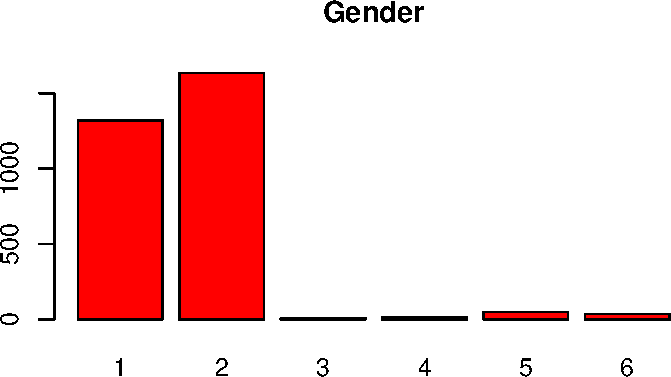
\includegraphics{./results_files/figure-pdf/fig-gender-DIF-1.pdf}

}

\caption{\label{fig-gender-DIF}Gender DIF}

\end{figure}

In this analysis, we examined the degree to which there was evidence of
uniform differential item functioning (DIF) between two subgroups of
participants (group 1 and group 2). As a first step we examined item
severity estimates and standard errors specific to each subgroup using
the Rating Scale Model Andrich (1978). We estimated item severity for
the two subgroups using a combined analysis of both subgroups and then
estimating the group-specific item severities and standard errors are
shown in Table X.

To examine the differences in item severity between subgroups, we
calculated standardized differences following Wright and Masters (1982)
as follows:

{[}equation{]}

where\\
z is the standardized difference, d1 is the item severity specific to
Subgroup 1, d2 is the item severity specific to Subgroup 2,\\
s e 2 1 is the standard error of the item severity specific to Subgroup
1, and\\
s e 2 2 is the standard error of the item severity specific to Subgroup
2. Using the formulation of the z statistic, higher values of z indicate
higher item locations (more-severe to endorse) for Subgroup 1 compared
to Subgroup 2.

Figure X shows a plot of the z-statistics for the four items; these
values are also presented numerically in Table X. In the figure, the
x-axis shows the item identification numbers, and the y-axis shows the
value of the z-statistic. Boundaries at +2 and -2 are indicated using
dashed horizontal lines to highlight statistically significant
differences in item severity between subgroups. Examination of these
results indicates that the items were not significantly different in
severity between the two subgroups. In addition, there were both
positive and negative z statistics, indicating that although the
differences in item severity were not significant, there were some items
that were easier to endorse for Subgroup 1 and others that were easier
to endorse for Subgroup 2.

Figure 1: Plot of Standardized Differences for Items between Subgroups

To further explore the differences in item severity between the two
subgroups, Figure 2 shows a scatterplot of the item locations between
the two subgroups. In the plot, the item severity for Subgroup 1 is
shown on the x-axis, and the item severity for Subgroup 2 is shown on
the y-axis. Individual items are indicated using open circle plotting
symbols. A solid identity line is included to highlight deviations from
invariant item severities between the two groups: Points that fall below
this line indicate that items were easier to endorse (lower item
measures) for Subgroup 2, and points that fall above the line indicate
that items were easier to endorse (lower item measures) for Subgroup 1.
Dashed lines are also included to indicate a 95\% confidence interval
for the difference between the item measures, following Luppescu (1995).

Figure 2: Scatterplot of Subgroup-Specific Item Severities

Finally, Figure 3 is a bar plot that illustrates the direction and
magnitude of the differences in item severities between subgroups. In
the plot, each bar represents the difference in severity between
subgroups for an individual item, ordered by the item sequence in the
survey. Bars that point to the left of the plot indicate that the item
was easier to endorse for Subgroup 1, and bars that point to the right
of the plot indicate that the item was easier to endorse for Subgroup 2.
Dashed vertical lines are plotted that show values of +0.5 and -0.5
logits as an indicator of substantial differences in item severity
between subgroups.

Figure 3: Bar Plot of Differences In Item Severity Between Subgroups

\bookmarksetup{startatroot}

\hypertarget{discussion}{%
\chapter*{Discussion}\label{discussion}}
\addcontentsline{toc}{chapter}{Discussion}

The purpose of this study was to further validate and enhance the
Spiritual Harm and Abuse Scale (SHAS) with the use of the Rasch Rating
Scale model. The present study improves upon the sample dependency of
factor analysis results and contributes new understanding about the
psychometric characteristics of the SHAS.

In this study, we examined unidimensionality, Rasch person/item
separation reliability, model-data fit, distribution of the variable map
based on the locations of persons and items, and individual item
qualities of the SHAS. In terms of dimensionality, we found satisfactory
evidence to unidimensionality to apply the Rasch Rating Scale model. We
found the SHAS highly reliable using Rasch person/item separation
reliability statistics, indicating that most of the items are sensitive
enough to capture different levels of spiritual abuse and most persons'
observed values overlap with the expected values. Similarly, there was
close correspondence between the data and the Rasch Rating Scale model
except for the outliers in the XXX ends of the continuum. This indicates
reasonable model-data fit. Regarding the variable map, our results
indicate that the SHAS, overall, captures a range of item severities
that reflect the order structure of spiritual abuse. However, we also
found a shortage of items at the very high and low ends of the
continuum. The SHAS can capture people who have experienced moderate
severity of spiritual abuse, but it is not sensitive enough to
discriminate among people who have experienced very severe and less
severe spiritual abuse. \textbackslash{[}For example, based on our Rasch
Rating scale model analysis, someone with a measure of − 3.00 logits and
another with a measure of − 2.00 logits would be more likely to respond
to the SHAS in the same way because there is no item on the scale that
targets very low levels of spiritual abuse. Hence, we would not be able
to detect which person has relatively more or less spiritual abuse in
comparison to each other. It would be similarly impossible to
distinguish levels of spiritual abuse between a person with a measure of
3.00 logits and another with a measure of 2.00 logits, and decide who
has experienced more severe spiritual abuse due to lack of items at the
high end of the continuum.\textbackslash{]} Finally, in terms of item
quality, XX of the XX items exhibited good psychometric quality, whereas
XX items were misfits. XXX items were redundant because they provided
the exact same information with identical pairs of each item, displaying
the same contributions to the sensitivity of the SHAS. Hence, they can
be removed from the scale to shorten the duration of administration.

Use of the Rasch measurement model in our study provided a powerful
analysis of the functioning of the SHAS at the item level and offered
in-depth insights on applicability of the scale in wider contexts due to
its sample independent nature. Whereas factor analytic approaches such
as exploratory factor analysis and confirmatory factor analysis do not
provide invariant measurement due to their sample dependency, the Rasch
measurement model is independent from the items that form the scale and
independent from the sample that the scale is administered to. This
feature will increase the applicability of the scale in wider contexts
and replicability of the present study in different populations due to
the possibility of direct application of the standards developed in one
study to data administered in another study (Yan and Mok 2012).

In conclusion, the results of this study provide strong evidence for the
validation of the SHAS despite the need for considering the deletion of
XX items that are misfits and of XX items that are redundant. The
revision or development of new items can also be considered to capture
gradations of challenges at the very high and low ends of the continuum
to detect people with very high and low levels of spiritual abuse.

\hypertarget{implications-and-future-directions}{%
\section*{Implications and future
directions}\label{implications-and-future-directions}}
\addcontentsline{toc}{section}{Implications and future directions}

This study presents the validation of the SHAS using the Rasch
measurement model, for assessing spiritual abuse in adults. The findings
have important implications for clinicians and researchers who are
concerned about spiritual abuse. The finding that the majority of the
SHAS items were of high quality implies that the items provide adequate
information to measure moderate levels of spiritual abuse. However, we
found the SHAS less able to distinguish people with very high and low
levels of spiritual abuse. Hence, for now clinicians and researchers
should be cautious when interpreting their results for people who have
very high and low spiritual abuse levels.

We echo the same limitations of these data noted in @KochEdstrom2022.
The SHAS was developed on a largely white and Protestant/former
Protestant population. Possibly major types or sub-themes of spiritual
abuse not captured here are more prominent in other religious
traditions. This would be a fruitful area of future study. Research into
spiritual abuse among the LGBTQ+ community might also yield insights
specific to that population. Future research could also distinguish
normed scores of this scale for different populations and denominations.

The final screener has the potential to both improve therapy for
innumerable clients who have experienced negative religious experiences
and to contribute a knowledge base for any future clinical training
around working with spiritually abused clients. The scale may also
contribute to future research that could be critical in understanding
not only the mechanisms and experience of spiritual abuse but also
perhaps the enduring power of religion, both to heal and to harm.

\bookmarksetup{startatroot}

\hypertarget{data-availability}{%
\chapter*{Data Availability}\label{data-availability}}
\addcontentsline{toc}{chapter}{Data Availability}

Data will be made available in accordance with xxx. Within one year of
publication of manuscripts addressing the aims of the grant,
investigators will make a deidentified, anonymized dataset available to
the public.

\bookmarksetup{startatroot}

\hypertarget{code-availability}{%
\chapter*{Code Availability}\label{code-availability}}
\addcontentsline{toc}{chapter}{Code Availability}

Code for the analyses presented in this paper will be made available
upon request.

\bookmarksetup{startatroot}

\hypertarget{acknowledgments}{%
\chapter*{Acknowledgments}\label{acknowledgments}}
\addcontentsline{toc}{chapter}{Acknowledgments}

This manuscript was not supported by grant funding. The views expressed
in this article are those of the authors and do not necessarily reflect
the position or policy of the Swedish Medical Center or Northwest
University.

\bookmarksetup{startatroot}

\hypertarget{funding}{%
\chapter*{Funding}\label{funding}}
\addcontentsline{toc}{chapter}{Funding}

This research was not supported by grant funding.

\bookmarksetup{startatroot}

\hypertarget{author-information}{%
\chapter*{Author Information}\label{author-information}}
\addcontentsline{toc}{chapter}{Author Information}

\hypertarget{affiliations}{%
\section*{Affiliations}\label{affiliations}}
\addcontentsline{toc}{section}{Affiliations}

\textbf{Department of Pharmacy, Swedish Medical Center, Seattle, USA}

Jack Huber

\textbf{Department of Psychology, Northwest University, Kirkland, USA}

Dan Koch

\hypertarget{corresponding-author}{%
\section*{Corresponding Author}\label{corresponding-author}}
\addcontentsline{toc}{section}{Corresponding Author}

Correspondence to \href{mailto:jack.bernard.huber@gmail.com}{Jack
Huber}.

\bookmarksetup{startatroot}

\hypertarget{ethics-declarations}{%
\chapter*{Ethics Declarations}\label{ethics-declarations}}
\addcontentsline{toc}{chapter}{Ethics Declarations}

\hypertarget{conflict-of-interest}{%
\section*{Conflict of Interest}\label{conflict-of-interest}}
\addcontentsline{toc}{section}{Conflict of Interest}

The authors declare no conflict of interest.

\bookmarksetup{startatroot}

\hypertarget{references}{%
\chapter*{References}\label{references}}
\addcontentsline{toc}{chapter}{References}

\hypertarget{refs}{}
\begin{CSLReferences}{1}{0}
\leavevmode\vadjust pre{\hypertarget{ref-Andrich1978}{}}%
Andrich, David. 1978. {``A Rating Formulation for Ordered Response
Categories.''} \emph{Psychometrika} 43: 561--73.

\leavevmode\vadjust pre{\hypertarget{ref-BondFox2015}{}}%
Bond, Trevor G., and Christine M. Fox. 2015. \emph{Applying the Rasch
Model: Fundamental Measurement in the Human Sciences}. New York, New
York: Routledge.

\leavevmode\vadjust pre{\hypertarget{ref-R-mirt}{}}%
Chalmers, Phil. 2022. \emph{Mirt: Multidimensional Item Response
Theory}. \url{https://CRAN.R-project.org/package=mirt}.

\leavevmode\vadjust pre{\hypertarget{ref-R-lordif}{}}%
Choi, Seung W., with contributions from Laura E. Gibbons, and Paul K.
Crane. 2016. \emph{Lordif: Logistic Ordinal Regression Differential Item
Functioning Using IRT}. \url{https://CRAN.R-project.org/package=lordif}.

\leavevmode\vadjust pre{\hypertarget{ref-Yen1984}{}}%
{``Effects of Local Item Dependence on the Fit and Equating Performance
of the Three-Parameter Logistic Model.''} 1984. \emph{Applied
Psychological Measurement} 8 (2): 125--45.

\leavevmode\vadjust pre{\hypertarget{ref-EmbretsonReise2000}{}}%
Embretson, Susan E., and Steven P. Reise. 2000. \emph{Item Response
Theory for Psychologists}. Mahwah, New Jerey: Lawrence Erlbaum
Associates.

\leavevmode\vadjust pre{\hypertarget{ref-Keller2016}{}}%
Keller, K. H. 2016. {``Development of a Spiritual Abuse
Questionnaire.''} PhD thesis, Texas Woman's University.

\leavevmode\vadjust pre{\hypertarget{ref-KochEdstrom2022}{}}%
Koch, Dan, and Leihua Edstrom. 2022. {``Development of the Spiritual
Harm and Abuse Scale.''} \emph{Journal for the Scientific Study of
Religion}.

\leavevmode\vadjust pre{\hypertarget{ref-R-eRm}{}}%
Mair, Patrick, Reinhold Hatzinger, and Marco J. Maier. 2021. \emph{eRm:
Extended Rasch Modeling}. \url{https://CRAN.R-project.org/package=eRm}.

\leavevmode\vadjust pre{\hypertarget{ref-R-base}{}}%
R Core Team. 2022. \emph{R: A Language and Environment for Statistical
Computing}. Vienna, Austria: R Foundation for Statistical Computing.
\url{https://www.R-project.org/}.

\leavevmode\vadjust pre{\hypertarget{ref-Rasch1960}{}}%
Rasch, Georg. 1960. \emph{Probabilistic Models for Some Intelligence and
Attainment Tests}. Chicago, IL: University of Chicago Press.

\leavevmode\vadjust pre{\hypertarget{ref-Reckase1979}{}}%
Reckase, Mark D. 1979. {``Unifactor Latent Trait Models Applied to
Multifactor Tests: Results and Implications.''} \emph{Journal of
Educational Statistics} 4: 207--30.

\leavevmode\vadjust pre{\hypertarget{ref-ReiseBonifayHaviland2013}{}}%
Reise, Steven P., Wes E. Bonifay, and Mark G. Haviland. 2013. {``Scoring
and Modeling Psychological Measures in the Presence of
Multidimensionality.''} \emph{Journal of Personality Assessment} 95 (2):
129--40. \url{https://doi.org/10.1080/00223891.2012.725437}.

\leavevmode\vadjust pre{\hypertarget{ref-ReiseMooreHaviland2013}{}}%
Reise, Steven P., Tyler M. Moore, and Mark G. Haviland. 2013.
{``Applying Unidimensional Item Response Theory Models to Psychological
Data.''} In \emph{APA Handbook of Testing and Assessment in Psychology:
Vol. 1. Test Theory and Testing and Assessment in Industrial and
Organizational Psychology}, 101--19.

\leavevmode\vadjust pre{\hypertarget{ref-ReiseWaller2009}{}}%
Reise, Steven P., and Niels G. Waller. 2009. {``Item Response Theory and
Clinical Measurement.''} \emph{Annual Review of Clinical Psychology} 5:
27--48. \url{https://doi.org/10.1146/annurev.clinpsy.032408.153553}.

\leavevmode\vadjust pre{\hypertarget{ref-R-psych}{}}%
Revelle, William. 2022. \emph{Psych: Procedures for Psychological,
Psychometric, and Personality Research}.
\href{https://personality-project.org/r/psych/\%0Ahttps://personality-project.org/r/psych-manual.pdf}{https://personality-project.org/r/psych/
https://personality-project.org/r/psych-manual.pdf}.

\leavevmode\vadjust pre{\hypertarget{ref-R-TAM}{}}%
Robitzsch, Alexander, Thomas Kiefer, and Margaret Wu. 2022. \emph{TAM:
Test Analysis Modules}. \url{https://CRAN.R-project.org/package=TAM}.

\end{CSLReferences}



\end{document}
